\documentclass[12pt]{article}\usepackage[]{graphicx}\usepackage[]{color}
%% maxwidth is the original width if it is less than linewidth
%% otherwise use linewidth (to make sure the graphics do not exceed the margin)
\makeatletter
\def\maxwidth{ %
  \ifdim\Gin@nat@width>\linewidth
    \linewidth
  \else
    \Gin@nat@width
  \fi
}
\makeatother

\definecolor{fgcolor}{rgb}{0.345, 0.345, 0.345}
\newcommand{\hlnum}[1]{\textcolor[rgb]{0.686,0.059,0.569}{#1}}%
\newcommand{\hlstr}[1]{\textcolor[rgb]{0.192,0.494,0.8}{#1}}%
\newcommand{\hlcom}[1]{\textcolor[rgb]{0.678,0.584,0.686}{\textit{#1}}}%
\newcommand{\hlopt}[1]{\textcolor[rgb]{0,0,0}{#1}}%
\newcommand{\hlstd}[1]{\textcolor[rgb]{0.345,0.345,0.345}{#1}}%
\newcommand{\hlkwa}[1]{\textcolor[rgb]{0.161,0.373,0.58}{\textbf{#1}}}%
\newcommand{\hlkwb}[1]{\textcolor[rgb]{0.69,0.353,0.396}{#1}}%
\newcommand{\hlkwc}[1]{\textcolor[rgb]{0.333,0.667,0.333}{#1}}%
\newcommand{\hlkwd}[1]{\textcolor[rgb]{0.737,0.353,0.396}{\textbf{#1}}}%

\usepackage{framed}
\makeatletter
\newenvironment{kframe}{%
 \def\at@end@of@kframe{}%
 \ifinner\ifhmode%
  \def\at@end@of@kframe{\end{minipage}}%
  \begin{minipage}{\columnwidth}%
 \fi\fi%
 \def\FrameCommand##1{\hskip\@totalleftmargin \hskip-\fboxsep
 \colorbox{shadecolor}{##1}\hskip-\fboxsep
     % There is no \\@totalrightmargin, so:
     \hskip-\linewidth \hskip-\@totalleftmargin \hskip\columnwidth}%
 \MakeFramed {\advance\hsize-\width
   \@totalleftmargin\z@ \linewidth\hsize
   \@setminipage}}%
 {\par\unskip\endMakeFramed%
 \at@end@of@kframe}
\makeatother

\definecolor{shadecolor}{rgb}{.97, .97, .97}
\definecolor{messagecolor}{rgb}{0, 0, 0}
\definecolor{warningcolor}{rgb}{1, 0, 1}
\definecolor{errorcolor}{rgb}{1, 0, 0}
\newenvironment{knitrout}{}{} % an empty environment to be redefined in TeX

\usepackage{alltt}
\usepackage[utf8]{inputenc}
\usepackage{graphicx}
\usepackage{color, colortbl}
\definecolor{blue1}{RGB}{0,102,204}
\usepackage[colorlinks = true,linkcolor = blue, citecolor = blue, urlcolor = blue]{hyperref}
\usepackage{array}
\usepackage[english]{babel}
\usepackage{amsfonts}
\usepackage{url}
\usepackage{pdflscape}
\usepackage{bm}
\usepackage[margin = 1.5cm]{geometry}
\usepackage[affil-it]{authblk}
\usepackage{hyperref}
\usepackage{multirow}
\usepackage[labelfont = bf]{caption}

\setlength{\doublerulesep}{0pt}
\newcommand{\R}{\mathbb{R}}
\newcommand{\code}[1]{{{\tt #1}}}

\let\oldtabular=\tabular
\def\tabular{\small\oldtabular}

\title{Appendix: Test the T-statistics using simulations: robustness and lack of bias in the function}
\author{Adrien Taudiere\thanks{\texttt{adrien.taudiere@cefe.cnrs.fr}} and Cyrille Violle}

\affil{{\footnotesize CEFE - Centre d'Ecologie Fonctionnelle et Evolutive, Montpellier: France}}

\date{\today}

\sloppy
\hyphenpenalty 10000



%%%%%%% Allow a subsubsub section  %%%%%%%%%
%%%%%%%%%%%%%%%%%%%%%%%%%%%%%%%%%%%%%%%%%%%%%%%%%%
\setcounter{secnumdepth}{4}
\setcounter{tocdepth}{4}
\makeatletter
\newcounter {subsubsubsection}[subsubsection]
\renewcommand\thesubsubsubsection{\thesubsubsection .\@arabic\c@subsubsubsection}
\newcommand\subsubsubsection{\@startsection{subsubsubsection}{4}{\z@}%
          {-3.25ex\@plus -1ex \@minus -.2ex}%
          {1.5ex \@plus .2ex}%
          {\normalfont\normalsize\bfseries}}
\renewcommand\paragraph{\@startsection{paragraph}{5}{\z@}%
         {3.25ex \@plus1ex \@minus.2ex}%
         {-1em}%
         {\normalfont\normalsize\bfseries}}
\renewcommand\subparagraph{\@startsection{subparagraph}{6}{\parindent}%
          {3.25ex \@plus1ex \@minus .2ex}%
          {-1em}%
          {\normalfont\normalsize\bfseries}}
\newcommand*\l@subsubsubsection{\@dottedtocline{4}{10.0em}{4.1em}}
\renewcommand*\l@paragraph{\@dottedtocline{5}{10em}{5em}}
\renewcommand*\l@subparagraph{\@dottedtocline{6}{12em}{6em}}
\newcommand*{\subsubsubsectionmark}[1]{}
\makeatother

\usepackage{hyperref}

\makeatletter
\def\toclevel@subsubsubsection{4}
\def\toclevel@paragraph{5}
\def\toclevel@subparagraph{6}
\makeatother


\definecolor{ligthgray}{RGB}{218, 218, 218}

%%%%%%%%%%%%%%%%%%%%%%%%%%%%%%%%%%%%%%%%%%%%%%%%%%
%%%%%%%%%%%%%%%%%%%%%%%%%%%%%%%%%%%%%%%%%%%%%%%%%%
%%%%%%%%%%%%%%%%%%%%%%%%%%%%%%%%%%%%%%%%%%%%%%%%%%
\IfFileExists{upquote.sty}{\usepackage{upquote}}{}
\begin{document}
\selectlanguage{english}




\maketitle

\begin{abstract}

\end{abstract}


\textbf{Key words:}
Functional space, functional structure, community assembly, ecological niche, environmental filter,
individual differences, intraspecific variation, null model, trait, variance decomposition


\vfill
\begin{center}
\textbf{To read a summary of this appendix, see directly section Summary \ref{sect:summary}.}
\textbf{An up to date version of the cati tutorial is available \href{http://sourceforge.net/p/cati-r/code/ci/master/tree/tutorial/vignettes/vignette.pdf}{here}.}
\end{center}

\newpage
\tableofcontents
\newpage


\section{Introduction}
 This document show the lack of bias in the functions \texttt{Tstats}, \texttt{partvar}, \texttt{decompCTRE} and a test of robustness for the T-statistics.
This report was created on 2015-01-21 11:49:28. Start directly by the summary section if you want condensate results of this document.

\subsection{R requirements}

First we need to install and load the package. 
\begin{knitrout}\small
\definecolor{shadecolor}{rgb}{0.969, 0.969, 0.969}\color{fgcolor}\begin{kframe}
\begin{alltt}
\hlcom{# install.packages("cati", repos = "http://cran.us.r-project.org", dependencies = TRUE)}
\hlkwd{library}\hlstd{(}\hlstr{"cati"}\hlstd{)}
\hlkwd{library}\hlstd{(}\hlstr{"xtable"}\hlstd{)}

\hlcom{# Save the graphical parameter}
\hlstd{oldpar} \hlkwb{<-} \hlkwd{par}\hlstd{(}\hlkwc{no.readonly} \hlstd{=} \hlnum{TRUE}\hlstd{)}
\end{alltt}
\end{kframe}
\end{knitrout}

  \subsection{System and session informations}
  This document was created with R version 3.1.2 (2014-10-31) on Windows. See below for more information. The speed computations of \texttt{cati} main functions are develop  in the \href{http://sourceforge.net/p/cati-r/code/ci/master/tree/tutorial/vignettes/vignette.pdf}{cati tutorial}.
  
\begin{knitrout}\small
\definecolor{shadecolor}{rgb}{0.969, 0.969, 0.969}\color{fgcolor}\begin{kframe}
\begin{alltt}
\hlkwd{sessionInfo}\hlstd{()}
\end{alltt}
\begin{verbatim}
## R version 3.1.2 (2014-10-31)
## Platform: x86_64-w64-mingw32/x64 (64-bit)
## 
## locale:
## [1] LC_COLLATE=French_France.1252  LC_CTYPE=French_France.1252   
## [3] LC_MONETARY=French_France.1252 LC_NUMERIC=C                  
## [5] LC_TIME=French_France.1252    
## 
## attached base packages:
## [1] stats     graphics  grDevices utils     datasets  methods   base     
## 
## other attached packages:
## [1] xtable_1.7-4 cati_0.94    ape_3.2      ade4_1.6-2   nlme_3.1-119
## [6] knitr_1.8   
## 
## loaded via a namespace (and not attached):
##  [1] class_7.3-11        codetools_0.2-9     digest_0.6.8       
##  [4] e1071_1.6-4         evaluate_0.5.5      formatR_1.0        
##  [7] geometry_0.3-5      grid_3.1.2          hexbin_1.27.0      
## [10] highr_0.4           hypervolume_1.1.1   igraph_0.7.1       
## [13] lattice_0.20-29     latticeExtra_0.6-26 magic_1.5-6        
## [16] MASS_7.3-35         mice_2.22           nnet_7.3-8         
## [19] randomForest_4.6-10 raster_2.3-12       rasterVis_0.32     
## [22] RColorBrewer_1.1-2  Rcpp_0.11.3         rgl_0.95.1201      
## [25] rpart_4.1-8         sp_1.0-16           stringr_0.6.2      
## [28] tools_3.1.2         zoo_1.7-11
\end{verbatim}
\end{kframe}
\end{knitrout}

  \subsection {T-statistics and associated null models}
  
  
\begin{landscape}
\begin{table}[h]
\caption[T-statistics and associated null models]{The four types of null models implemented in cati, their related null and alternative hypotheses, randomization design and associated T-statistics}
\begin{tabular}{m{2.7cm} m{5.3cm} m{6.3cm} m{6.2cm} m{2.5cm}}

& Null hypothesis & Randomization procedure & Unilateral alternative hypothesis & T-statistics  \tabularnewline
\hline \hline \hline

local & There is no internal filtering: the distribution of trait values of all individuals within a given community does not depend on species identity & Randomization of individual trait values within the community& Internal filtering significantly impacts the distribution of trait values within a given community: two individuals belonging to a population have more similar trait values than two individuals randomly-drawn in the community & $T_{IP/IC}$   \tabularnewline

\hline

regional.ind  & There is no external filtering: the distribution of trait values of individuals within a given community is a random drawing from the regional pool & Draw without replacement of individual trait values belonging to the regional pool (keeping the actual number of individuals in each community) & Two individuals belonging to a community have more similar trait values than two individuals randomly-drawn in the regional pool & $T_{IC/IR}$\tabularnewline

\hline

regional.pop \& regional.pop.prab & There is no species-based external filtering: the distribution of mean trait values of species within a given community is a random draw from the regional pool & (i) Assignment of a population-level value to each individual and (ii) Draw without replacement of population-level trait values belonging to the regional pool (keeping the actual number of individuals in each community (regional.pop) or not (regional.pop .prab). & Two individuals belonging to a community have more similar population-based trait values than two individuals randomly-drawn in the regional pool with (regional.pop) or without (regional.pop .prab) taking abundance into account. & $T_{PC/PR}$  (regional.pop) \tabularnewline


\end{tabular}
\end{table}
\end{landscape}


  
  
  
  
  
  
  \subsection{Simulations parameters}

Here we define the number of permutations for the entire analysis. 

\begin{knitrout}\small
\definecolor{shadecolor}{rgb}{0.969, 0.969, 0.969}\color{fgcolor}\begin{kframe}
\begin{alltt}
\hlcom{#Number of permutations for the analysis with no filter}
\hlstd{npermut} \hlkwb{<-} \hlnum{1000}

\hlcom{#Number of permutations for each parameters values in the analysis with filter(s)}
\hlstd{N_repet_Param} \hlkwb{<-} \hlnum{200}

\hlcom{#Number of values for each parameters}
\hlstd{nb_param_val} \hlkwb{<-} \hlnum{10}
\end{alltt}
\end{kframe}
\end{knitrout}

\begin{knitrout}\small
\definecolor{shadecolor}{rgb}{0.969, 0.969, 0.969}\color{fgcolor}\begin{kframe}
\begin{alltt}
\hlcom{#Parameter of the log normal distribution for species abundances }
\hlcom{#distribution within communities}
\hlstd{sdlog} \hlkwb{=} \hlnum{1.5}

\hlcom{#Ten communities named A, B, C ... J}
\hlstd{com} \hlkwb{<-} \hlkwd{c}\hlstd{(}\hlstr{"A"}\hlstd{,} \hlstr{"B"}\hlstd{,} \hlstr{"C"}\hlstd{,} \hlstr{"D"}\hlstd{,} \hlstr{"E"}\hlstd{,} \hlstr{"F"}\hlstd{,} \hlstr{"G"}\hlstd{,} \hlstr{"H"}\hlstd{,} \hlstr{"I"}\hlstd{,} \hlstr{"J"}\hlstd{)}
\hlstd{Ncom} \hlkwb{<-} \hlkwd{length}\hlstd{(com)}

\hlcom{#Twenty species sp1, sp2, sp3, ... sp20}
\hlstd{sp} \hlkwb{<-} \hlkwd{paste}\hlstd{(}\hlstr{"sp"}\hlstd{,} \hlkwd{seq}\hlstd{(}\hlnum{1}\hlopt{:}\hlnum{20}\hlstd{),} \hlkwc{sep} \hlstd{=} \hlstr{""}\hlstd{)}
\hlstd{Nsp} \hlkwb{<-} \hlkwd{length}\hlstd{(sp)}

\hlcom{#Total number of individuals}
\hlstd{Nind} \hlkwb{<-} \hlnum{1000}
\end{alltt}
\end{kframe}
\end{knitrout}

\begin{figure}[h]
\centering
\hspace*{-0.8cm}
\vspace*{-0.5cm}
    \makebox[\linewidth]{
        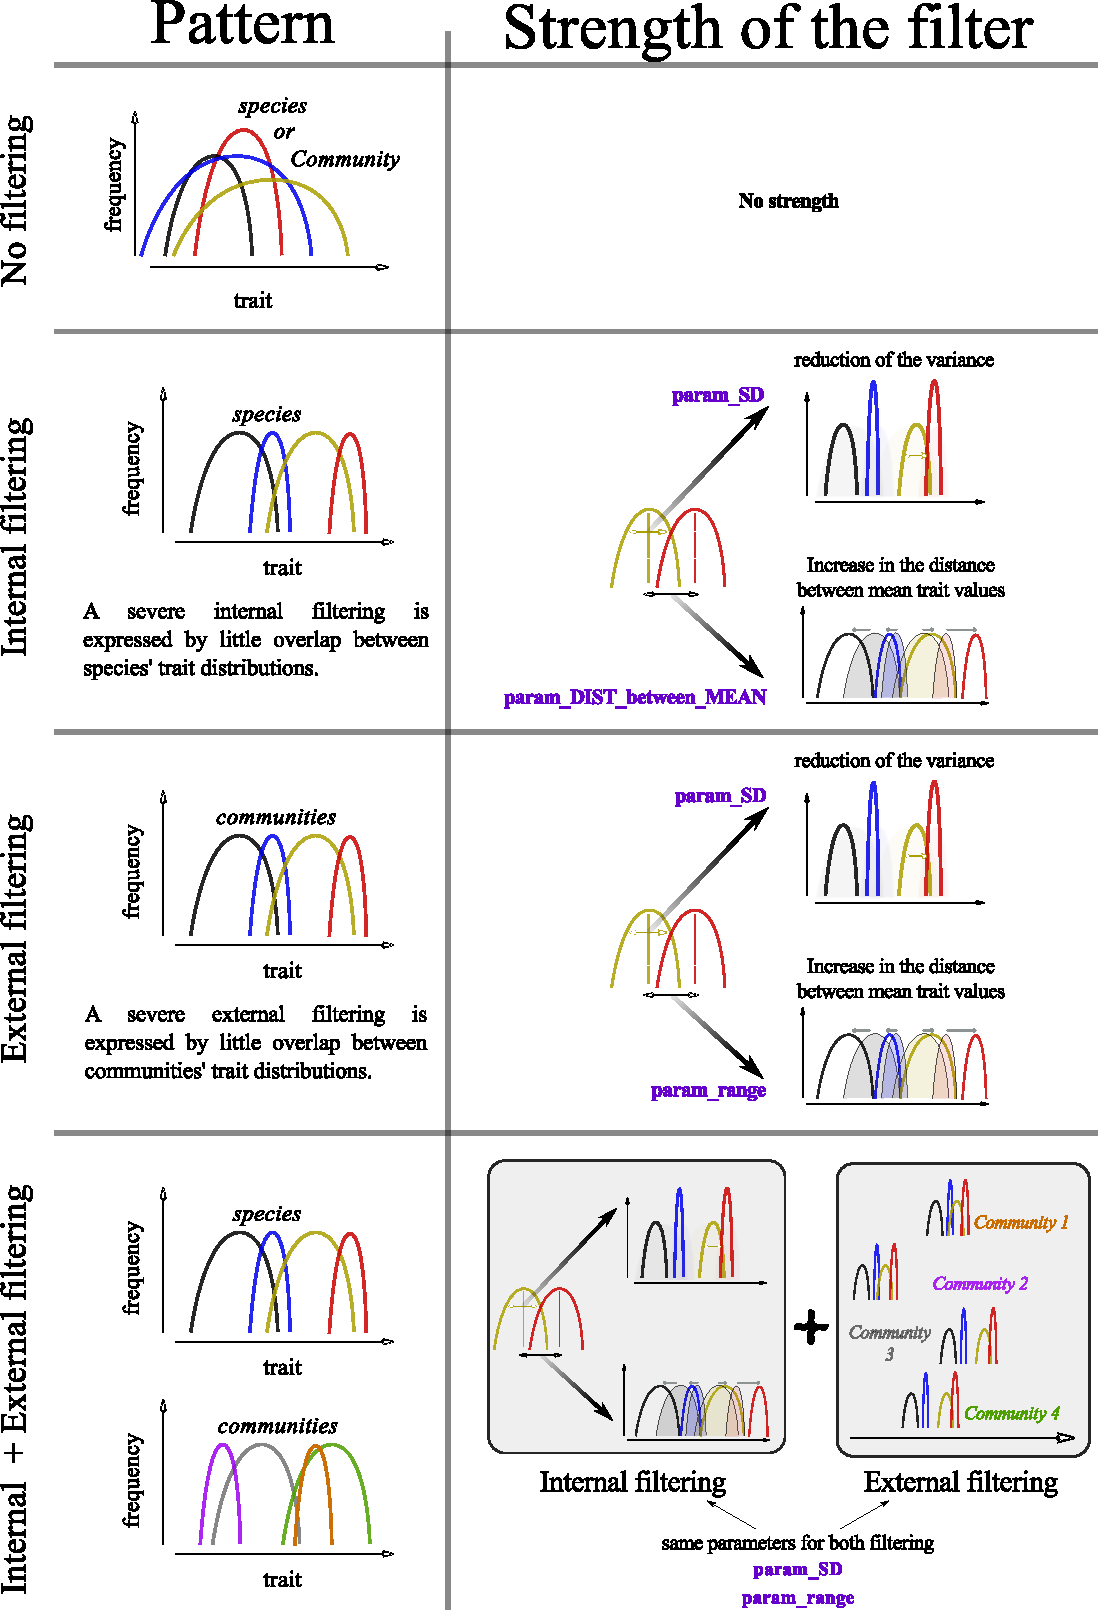
\includegraphics[width=0.9\linewidth]{general_outline.pdf}
    }
\caption[General outline of the simulation concerning the Tstatistics]{General outline of the simulation concerning the Tstatistics. (Continue on next page) }
\label{fig:General_outline}
\end{figure}

\clearpage
\textbf{Figure 1 (continue):} The \textbf{absence of filtering} is use to test the type I error (alpha-error) of the three Tstatistics. In the absence of filtering the expected pattern is a random distribution of individual traits values into species and communities. \textbf{Internal filter} includes all of the assembly processes internal to the community. The alternative hypothesis (thus the expected pattern) of habitat filtering is the non overlap between species traits distributions measured by the ratio $T_{IP/IC}$. We modulate the strength of filter in the simulation using the variance of species traits distributions and the distance between species traits means. \textbf{External filter} includes all of the assembly processes external to the community. In this document we specifically treat the case of an environnemental gradient influencing the individual traits values. Thus the expected pattern a non overlap between communities traits distributions measured by the ratio $T_{IC/IR}$ and its populationnal counterparts. We modulate the strength of external filter in the simulation using the variance of communities traits distributions and the range of communities traits means (the "extent" of the environnemental gradient). Finally, we add external filter to internal filter by adding to each individual values of the internal filter simulation a number depending of the community distribution.
\vspace*{1cm}

We use toys models of 1000 individuals belonging to 20 species occuring in 10 communities (sites). Each community contains 100 individuals and species abundances in each community are defined following a lognormal distribution of mean 0 and standard deviation \texttt{sdlog} of 1.5.
Figure \ref{fig:General_outline} depict the general outline of the next fourth sections dealing with the statistical test of T-statistics from Violle \textit{et al.} (2012).



\cleardoublepage

\section{No filter: calculation of error}
 \subsection {Randomization outline}

To calculate the \textbf{alpha error} (\textit{i.e.} the probability of rejected the null hypothesis H0 while H0 is true), we draw 1000 random traits matrix irrespective of the species and community attributes of each individuals.

\begin{knitrout}\small
\definecolor{shadecolor}{rgb}{0.969, 0.969, 0.969}\color{fgcolor}\begin{kframe}
\begin{alltt}
\hlcom{#Start simulation }
\hlstd{res.simu1} \hlkwb{<-} \hlkwd{list}\hlstd{() ; res.simu1.pval} \hlkwb{<-} \hlkwd{list}\hlstd{()}

\hlkwa{for}\hlstd{(n} \hlkwa{in} \hlnum{1}\hlopt{:}\hlstd{npermut)\{}\hlcom{#for each permutation}

 \hlstd{ex.traits1} \hlkwb{<-} \hlkwd{array}\hlstd{(}\hlnum{NA}\hlstd{,} \hlkwc{dim} \hlstd{=} \hlkwd{c}\hlstd{(Nind,} \hlnum{2}\hlstd{))}
 \hlkwd{colnames}\hlstd{(ex.traits1)} \hlkwb{<-} \hlkwd{paste}\hlstd{(}\hlstr{"trait"}\hlstd{,} \hlkwd{c}\hlstd{(}\hlstr{"a"}\hlstd{,} \hlstr{"b"}\hlstd{),} \hlkwc{sep} \hlstd{=} \hlstr{" "}\hlstd{)}

 \hlcom{#trait a: normal distribution}
 \hlstd{ex.traits1[,} \hlnum{1}\hlstd{]} \hlkwb{<-} \hlkwd{rnorm}\hlstd{(Nind,} \hlkwd{rlnorm}\hlstd{(Nind,} \hlnum{0}\hlstd{,} \hlnum{1}\hlstd{),} \hlkwd{rlnorm}\hlstd{(Nind,} \hlnum{0}\hlstd{,} \hlnum{1}\hlstd{))}

 \hlcom{#trait b: uniform distribution}
 \hlstd{ex.traits1[,} \hlnum{2}\hlstd{]} \hlkwb{<-} \hlkwd{runif}\hlstd{(Nind)}

 \hlcom{# Draw communities using lognormal distribution of abondances }
 \hlstd{ex.sp1} \hlkwb{<-} \hlkwd{c}\hlstd{()}
 \hlstd{ex.com1} \hlkwb{<-} \hlkwd{matrix}\hlstd{(}\hlnum{0}\hlstd{,} \hlkwc{nrow} \hlstd{= Ncom,} \hlkwc{ncol} \hlstd{= Nsp)}
 \hlkwa{for}\hlstd{(c} \hlkwa{in} \hlnum{1}\hlopt{:} \hlstd{Ncom)\{}
  \hlstd{ex.com.interm} \hlkwb{<-} \hlkwd{table}\hlstd{(}\hlkwd{sample}\hlstd{(sp,} \hlkwc{size} \hlstd{= Nind} \hlopt{/} \hlstd{Ncom,} \hlkwc{prob} \hlstd{=} \hlkwd{rlnorm}\hlstd{(Nsp,} \hlnum{0}\hlstd{, sdlog),}
                                \hlkwc{replace} \hlstd{= T))}

  \hlstd{ex.com1[c, sp} \hlopt \hlkwd{names}\hlstd{(ex.com.interm)]} \hlkwb{<-} \hlstd{ex.com.interm}

  \hlstd{ex.sp1} \hlkwb{<-} \hlkwd{c}\hlstd{(ex.sp1,} \hlkwd{rep}\hlstd{(sp,} \hlkwc{times} \hlstd{= ex.com1[c,]))}
 \hlstd{\}}
 \hlstd{ex.indplot1} \hlkwb{<-} \hlkwd{as.factor}\hlstd{(}\hlkwd{rep}\hlstd{(com,} \hlnum{100}\hlstd{))}


 \hlcom{#Stock the results}
 \hlstd{res.simu1[[n]]} \hlkwb{<-} \hlkwd{Tstats}\hlstd{(ex.traits1, ex.indplot1, ex.sp1)}
 \hlstd{res.simu1.pval[[n]]} \hlkwb{<-} \hlkwd{sum_Tstats}\hlstd{(res.simu1[[n]],} \hlkwc{type} \hlstd{=} \hlstr{"p.value"}\hlstd{)}
 \hlkwd{print}\hlstd{(}\hlkwd{paste}\hlstd{(}\hlstr{"---"}\hlstd{,} \hlkwd{round}\hlstd{(n}\hlopt{/}\hlstd{npermut,} \hlnum{2}\hlstd{)} \hlopt{*} \hlnum{100}\hlstd{,} \hlstr{"%"}\hlstd{,} \hlkwc{sep} \hlstd{=} \hlstr{" "}\hlstd{))}
\hlstd{\}}\hlcom{#end of simulation}
\end{alltt}
\end{kframe}
\end{knitrout}

  \subsection {Results for simulations with no filtering}
Let's see the result for one typical randomization. We can plot the distribution of traits within species and/or communities thanks to the function \texttt{plotDistri} (Fig. \ref{fig:No_Filter_plots}). We can also plot the result of the T-statistics for one of the 1000 permutations (Fig. \ref{fig:No_Filter_plots_Tstats}).

\begin{knitrout}\small
\definecolor{shadecolor}{rgb}{0.969, 0.969, 0.969}\color{fgcolor}\begin{kframe}
\begin{alltt}
\hlkwd{par}\hlstd{(}\hlkwc{mfrow}\hlstd{=}\hlkwd{c}\hlstd{(}\hlnum{2}\hlstd{,} \hlnum{2}\hlstd{))}
\hlkwd{plotDistri}\hlstd{(ex.traits1,} \hlkwd{rep}\hlstd{(}\hlstr{"all_sp"}\hlstd{,} \hlkwc{times} \hlstd{=} \hlkwd{dim}\hlstd{(ex.traits1)[}\hlnum{1}\hlstd{]), ex.indplot1,}
           \hlkwc{plot.ask} \hlstd{= F,} \hlkwc{multipanel} \hlstd{= F,} \hlkwc{leg} \hlstd{=}\hlkwd{c}\hlstd{(T, F),} \hlkwc{main} \hlstd{=} \hlkwd{c}\hlstd{(}\hlstr{"a"}\hlstd{,} \hlstr{"b"}\hlstd{))}
\hlkwd{plotDistri}\hlstd{(ex.traits1,} \hlkwd{rep}\hlstd{(}\hlstr{"region"}\hlstd{,} \hlkwc{times} \hlstd{=} \hlkwd{dim}\hlstd{(ex.traits1)[}\hlnum{1}\hlstd{]), ex.sp1,}
           \hlkwc{plot.ask} \hlstd{= F,} \hlkwc{multipanel} \hlstd{= F,} \hlkwc{leg} \hlstd{=}\hlkwd{c}\hlstd{(T, F),} \hlkwc{main} \hlstd{=} \hlkwd{c}\hlstd{(}\hlstr{"c"}\hlstd{,} \hlstr{"d"}\hlstd{))}
\hlkwd{par}\hlstd{(}\hlkwc{mfrow}\hlstd{=}\hlkwd{c}\hlstd{(}\hlnum{1}\hlstd{,} \hlnum{1}\hlstd{))}
\end{alltt}
\end{kframe}\begin{figure}

{\centering 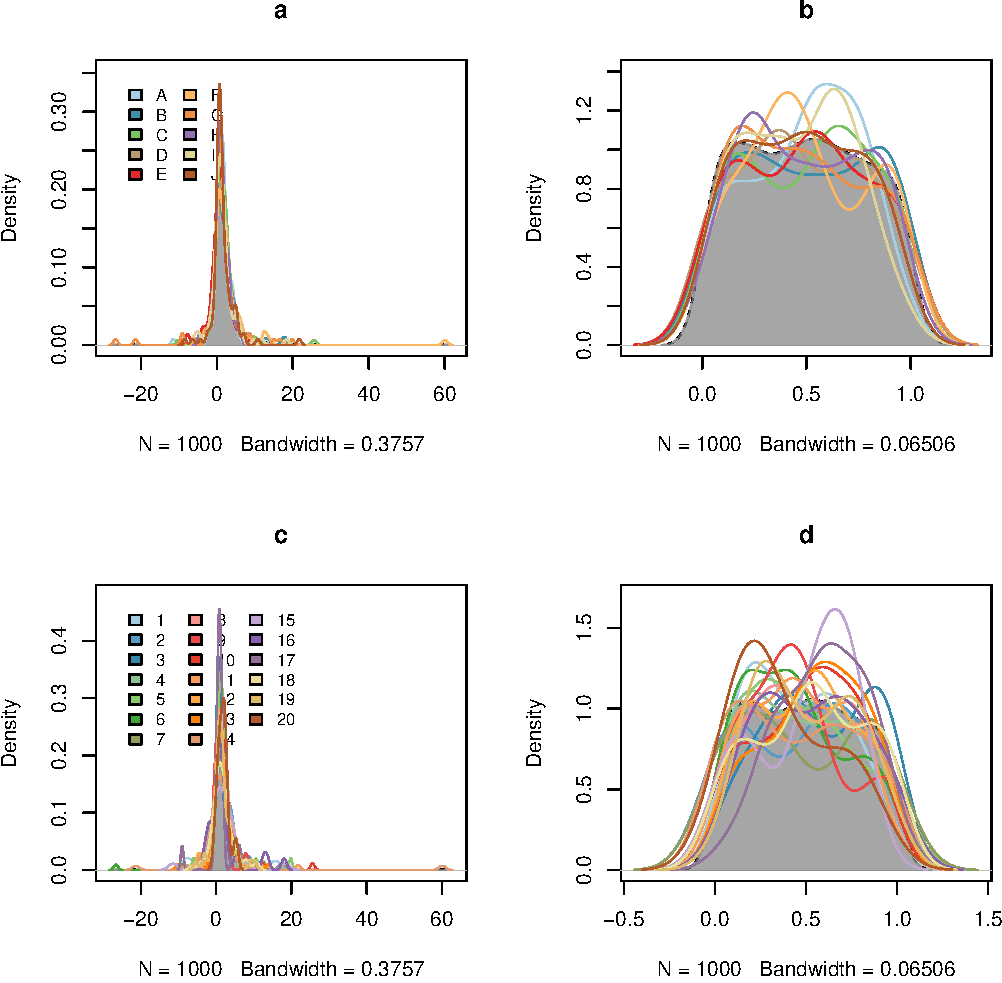
\includegraphics[width=\maxwidth]{figure/No_Filter_plots-1} 

}

\caption[Distribution of traits for one randomization without filter]{Distribution of traits for one randomization without filter: (a) Communities trait distributions for the trait a (normal distribution); (b) Communities trait distributions for the trait b (uniform distribution); (c) Species trait distributions for the trait a; (d) Species trait distributions for the trait b\label{fig:No_Filter_plots}}
\end{figure}


\end{knitrout}

\begin{knitrout}\small
\definecolor{shadecolor}{rgb}{0.969, 0.969, 0.969}\color{fgcolor}\begin{kframe}
\begin{alltt}
\hlkwd{plot}\hlstd{(res.simu1[[}\hlnum{1}\hlstd{]])}
\end{alltt}
\end{kframe}\begin{figure}

{\centering 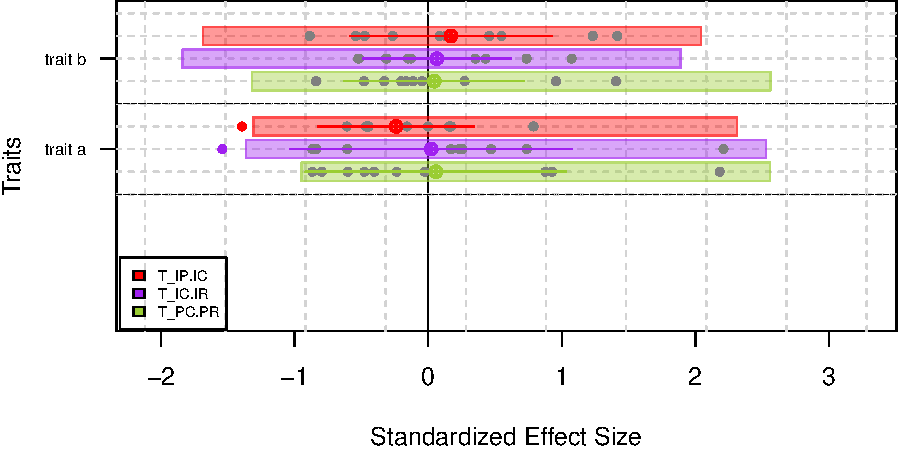
\includegraphics[width=\maxwidth]{figure/No_Filter_plots_Tstats-1} 

}

\caption[Results of T-statistics for one randomization without filter]{Results of T-statistics for one randomization without filter: $T_{IP/IC}$ in red, $T_{IC/IR}$ in purple and $T_{PC/PR}$ in green.\label{fig:No_Filter_plots_Tstats}}
\end{figure}


\end{knitrout}

 \subsection {Assess the statistical type I error of local T-statistics}
 
Here we call local p-values the p-values corresponding to one indice for one trait in one community \footnote{In contrast with global statistics which aggregate the communities values metrics.}. Now lets plot the results as the ordered p.value for each T-statistics and each traits (Fig. \ref{fig:No_Filter_results})). In that case we have 20 p-values \footnote{10 p-value, corresponding to 10 communities, multiply by 2 because we are doing a bilateral test} by T-statistics by traits for each permutation. Using the defined parameters, we plot \ensuremath{2\times 10^{4}} points by T-statistic by trait (20 p.value multiply by 1000 permutation). 

The alpha error on the figure are the proportion of p.value which are inferior to 0.025 (because we are doing a bilateral test).

\begin{knitrout}\small
\definecolor{shadecolor}{rgb}{0.969, 0.969, 0.969}\color{fgcolor}\begin{kframe}
\begin{alltt}
\hlkwd{par}\hlstd{(}\hlkwc{mfrow} \hlstd{=} \hlkwd{c}\hlstd{(}\hlnum{3}\hlstd{,} \hlnum{2}\hlstd{))}
\hlkwd{par}\hlstd{(}\hlkwc{mar} \hlstd{=} \hlkwd{c}\hlstd{(}\hlnum{3}\hlstd{,} \hlnum{3.5}\hlstd{,} \hlnum{2}\hlstd{,} \hlnum{0.2}\hlstd{))}

\hlstd{xx} \hlkwb{<-} \hlkwd{log10}\hlstd{(}\hlkwd{sort}\hlstd{(}\hlkwd{unlist}\hlstd{(}\hlkwd{lapply}\hlstd{(res.simu1.pval,} \hlkwa{function}\hlstd{(}\hlkwc{x}\hlstd{) x[}\hlnum{1}\hlopt{:}\hlnum{20}\hlstd{,} \hlnum{1}\hlstd{]))))}
\hlkwd{plot}\hlstd{(xx,} \hlkwc{type} \hlstd{=} \hlstr{"l"}\hlstd{,} \hlkwc{main} \hlstd{=} \hlstr{"T_IP.IC norm"}\hlstd{,} \hlkwc{ylab} \hlstd{=} \hlnum{NA} \hlstd{,} \hlkwc{xlab} \hlstd{=} \hlnum{NA}\hlstd{)}
\hlkwd{abline}\hlstd{(}\hlkwc{h} \hlstd{=} \hlkwd{log10}\hlstd{(}\hlnum{0.025}\hlstd{))}
\hlstd{nbre_alpha_error_norm_loc_Tipic} \hlkwb{<-} \hlkwd{round}\hlstd{((}\hlkwd{sum}\hlstd{(xx} \hlopt{<} \hlkwd{log10}\hlstd{(}\hlnum{0.025}\hlstd{))} \hlopt{+}\hlnum{1} \hlstd{)} \hlopt{/} \hlstd{(}\hlkwd{length}\hlstd{(xx)}\hlopt{+}\hlnum{1}\hlstd{),} \hlnum{5}\hlstd{)}
\hlkwd{text}\hlstd{(}\hlnum{0}\hlstd{,} \hlopt{-}\hlnum{0.3}\hlstd{,} \hlkwc{labels} \hlstd{=} \hlkwd{paste}\hlstd{(}\hlstr{"alpha error"}\hlstd{, nbre_alpha_error_norm_loc_Tipic,} \hlkwc{sep} \hlstd{=} \hlstr{" = "}\hlstd{),}
     \hlkwc{pos} \hlstd{=} \hlnum{4}\hlstd{)}
\hlkwd{mtext}\hlstd{(}\hlstr{"log10 pvalue"}\hlstd{,} \hlnum{2}\hlstd{,} \hlkwc{line} \hlstd{=} \hlnum{2}\hlstd{)}

\hlstd{xx} \hlkwb{<-} \hlkwd{log10}\hlstd{(}\hlkwd{sort}\hlstd{(}\hlkwd{unlist}\hlstd{(}\hlkwd{lapply}\hlstd{(res.simu1.pval,} \hlkwa{function}\hlstd{(}\hlkwc{x}\hlstd{) x[}\hlnum{1}\hlopt{:}\hlnum{20}\hlstd{,} \hlnum{2}\hlstd{]))))}
\hlkwd{plot}\hlstd{(xx,} \hlkwc{type} \hlstd{=} \hlstr{"l"}\hlstd{,} \hlkwc{main} \hlstd{=} \hlstr{"T_IP.IC Uni"}\hlstd{,} \hlkwc{ylab} \hlstd{=} \hlnum{NA}\hlstd{,} \hlkwc{xlab} \hlstd{=} \hlnum{NA}\hlstd{)}
\hlkwd{abline}\hlstd{(}\hlkwc{h} \hlstd{=} \hlkwd{log10}\hlstd{(}\hlnum{0.025}\hlstd{))}
\hlstd{nbre_alpha_error_uni_loc_Tipic} \hlkwb{<-} \hlkwd{round}\hlstd{((}\hlkwd{sum}\hlstd{(xx} \hlopt{<} \hlkwd{log10}\hlstd{(}\hlnum{0.025}\hlstd{))} \hlopt{+}\hlnum{1} \hlstd{)} \hlopt{/} \hlstd{(}\hlkwd{length}\hlstd{(xx)}\hlopt{+}\hlnum{1}\hlstd{),} \hlnum{5}\hlstd{)}
\hlkwd{text}\hlstd{(}\hlnum{0}\hlstd{,} \hlopt{-}\hlnum{0.3}\hlstd{,} \hlkwc{labels} \hlstd{=} \hlkwd{paste}\hlstd{(}\hlstr{"alpha error"}\hlstd{, nbre_alpha_error_uni_loc_Tipic,} \hlkwc{sep} \hlstd{=} \hlstr{" = "}\hlstd{),}
     \hlkwc{pos} \hlstd{=} \hlnum{4}\hlstd{)}

\hlstd{xx} \hlkwb{<-} \hlkwd{log10}\hlstd{(}\hlkwd{sort}\hlstd{(}\hlkwd{unlist}\hlstd{(}\hlkwd{lapply}\hlstd{(res.simu1.pval,} \hlkwa{function}\hlstd{(}\hlkwc{x}\hlstd{) x[}\hlnum{21}\hlopt{:}\hlnum{40}\hlstd{,} \hlnum{1}\hlstd{]))))}
\hlkwd{plot}\hlstd{(xx,} \hlkwc{type} \hlstd{=} \hlstr{"l"}\hlstd{,} \hlkwc{main} \hlstd{=} \hlstr{"T_IC.IR norm"}\hlstd{,} \hlkwc{ylab} \hlstd{=} \hlnum{NA}\hlstd{,} \hlkwc{xlab} \hlstd{=} \hlnum{NA}\hlstd{)}
\hlkwd{abline}\hlstd{(}\hlkwc{h} \hlstd{=} \hlkwd{log10}\hlstd{(}\hlnum{0.025}\hlstd{))}
\hlstd{nbre_alpha_error_norm_loc_Ticir} \hlkwb{<-} \hlkwd{round}\hlstd{((}\hlkwd{sum}\hlstd{(xx} \hlopt{<} \hlkwd{log10}\hlstd{(}\hlnum{0.025}\hlstd{))} \hlopt{+}\hlnum{1} \hlstd{)} \hlopt{/} \hlstd{(}\hlkwd{length}\hlstd{(xx)}\hlopt{+}\hlnum{1}\hlstd{),} \hlnum{5}\hlstd{)}
\hlkwd{text}\hlstd{(}\hlnum{0}\hlstd{,} \hlopt{-}\hlnum{0.3}\hlstd{,} \hlkwc{labels} \hlstd{=} \hlkwd{paste}\hlstd{(}\hlstr{"alpha error"}\hlstd{, nbre_alpha_error_norm_loc_Ticir,} \hlkwc{sep} \hlstd{=} \hlstr{" = "}\hlstd{),}
     \hlkwc{pos} \hlstd{=} \hlnum{4}\hlstd{)}
\hlkwd{mtext}\hlstd{(}\hlstr{"log10 pvalue"}\hlstd{,} \hlnum{2}\hlstd{,} \hlkwc{line} \hlstd{=} \hlnum{2}\hlstd{)}

\hlstd{xx} \hlkwb{<-} \hlkwd{log10}\hlstd{(}\hlkwd{sort}\hlstd{(}\hlkwd{unlist}\hlstd{(}\hlkwd{lapply}\hlstd{(res.simu1.pval,} \hlkwa{function}\hlstd{(}\hlkwc{x}\hlstd{) x[}\hlnum{21}\hlopt{:}\hlnum{40}\hlstd{,} \hlnum{2}\hlstd{]))))}
\hlkwd{plot}\hlstd{(xx,} \hlkwc{type} \hlstd{=} \hlstr{"l"}\hlstd{,} \hlkwc{main} \hlstd{=} \hlstr{"T_IC.IR Uni"}\hlstd{,} \hlkwc{ylab} \hlstd{=} \hlnum{NA}\hlstd{,} \hlkwc{xlab} \hlstd{=} \hlnum{NA}\hlstd{)}
\hlkwd{abline}\hlstd{(}\hlkwc{h} \hlstd{=} \hlkwd{log10}\hlstd{(}\hlnum{0.025}\hlstd{))}
\hlstd{nbre_alpha_error_uni_loc_Ticir} \hlkwb{<-} \hlkwd{round}\hlstd{((}\hlkwd{sum}\hlstd{(xx} \hlopt{<} \hlkwd{log10}\hlstd{(}\hlnum{0.025}\hlstd{))} \hlopt{+}\hlnum{1} \hlstd{)} \hlopt{/} \hlstd{(}\hlkwd{length}\hlstd{(xx)}\hlopt{+}\hlnum{1}\hlstd{),} \hlnum{5}\hlstd{)}
\hlkwd{text}\hlstd{(}\hlnum{0}\hlstd{,} \hlopt{-}\hlnum{0.3}\hlstd{,} \hlkwc{labels} \hlstd{=} \hlkwd{paste}\hlstd{(}\hlstr{"alpha error"}\hlstd{, nbre_alpha_error_uni_loc_Ticir,} \hlkwc{sep} \hlstd{=} \hlstr{" = "}\hlstd{),}
     \hlkwc{pos} \hlstd{=} \hlnum{4}\hlstd{)}

\hlstd{xx} \hlkwb{<-} \hlkwd{log10}\hlstd{(}\hlkwd{sort}\hlstd{(}\hlkwd{unlist}\hlstd{(}\hlkwd{lapply}\hlstd{(res.simu1.pval,} \hlkwa{function}\hlstd{(}\hlkwc{x}\hlstd{) x[}\hlnum{41}\hlopt{:}\hlnum{60}\hlstd{,} \hlnum{1}\hlstd{]))))}
\hlkwd{plot}\hlstd{(xx,} \hlkwc{type} \hlstd{=} \hlstr{"l"}\hlstd{,} \hlkwc{main} \hlstd{=} \hlstr{"T_PC.PR norm"}\hlstd{,} \hlkwc{ylab} \hlstd{=} \hlnum{NA}\hlstd{,} \hlkwc{xlab} \hlstd{=} \hlnum{NA}\hlstd{)}
\hlkwd{abline}\hlstd{(}\hlkwc{h} \hlstd{=} \hlkwd{log10}\hlstd{(}\hlnum{0.025}\hlstd{))}
\hlstd{nbre_alpha_error_norm_loc_Tpcpr} \hlkwb{<-} \hlkwd{round}\hlstd{((}\hlkwd{sum}\hlstd{(xx} \hlopt{<} \hlkwd{log10}\hlstd{(}\hlnum{0.025}\hlstd{))} \hlopt{+}\hlnum{1} \hlstd{)} \hlopt{/} \hlstd{(}\hlkwd{length}\hlstd{(xx)}\hlopt{+}\hlnum{1}\hlstd{),} \hlnum{5}\hlstd{)}
\hlkwd{text}\hlstd{(}\hlnum{0}\hlstd{,} \hlopt{-}\hlnum{0.3}\hlstd{,} \hlkwc{labels} \hlstd{=} \hlkwd{paste}\hlstd{(}\hlstr{"alpha error"}\hlstd{, nbre_alpha_error_norm_loc_Tpcpr,} \hlkwc{sep} \hlstd{=} \hlstr{" = "}\hlstd{),}
     \hlkwc{pos} \hlstd{=} \hlnum{4}\hlstd{)}
\hlkwd{mtext}\hlstd{(}\hlstr{"log10 pvalue"}\hlstd{,} \hlnum{2}\hlstd{,} \hlkwc{line} \hlstd{=} \hlnum{2}\hlstd{)}
\hlkwd{mtext}\hlstd{(}\hlstr{"rank"}\hlstd{,} \hlnum{1}\hlstd{,} \hlkwc{line} \hlstd{=} \hlnum{2}\hlstd{)}

\hlstd{xx} \hlkwb{<-} \hlkwd{log10}\hlstd{(}\hlkwd{sort}\hlstd{(}\hlkwd{unlist}\hlstd{(}\hlkwd{lapply}\hlstd{(res.simu1.pval,} \hlkwa{function}\hlstd{(}\hlkwc{x}\hlstd{) x[}\hlnum{41}\hlopt{:}\hlnum{60}\hlstd{,} \hlnum{2}\hlstd{]))))}
\hlkwd{plot}\hlstd{(xx,} \hlkwc{type} \hlstd{=} \hlstr{"l"}\hlstd{,} \hlkwc{main} \hlstd{=} \hlstr{"T_PC.PR Uni"}\hlstd{,} \hlkwc{ylab} \hlstd{=} \hlnum{NA}\hlstd{,} \hlkwc{xlab} \hlstd{=} \hlnum{NA}\hlstd{)}
\hlkwd{abline}\hlstd{(}\hlkwc{h} \hlstd{=} \hlkwd{log10}\hlstd{(}\hlnum{0.025}\hlstd{))}
\hlstd{nbre_alpha_error_uni_loc_Tpcpr} \hlkwb{<-} \hlkwd{round}\hlstd{((}\hlkwd{sum}\hlstd{(xx} \hlopt{<} \hlkwd{log10}\hlstd{(}\hlnum{0.025}\hlstd{))} \hlopt{+}\hlnum{1} \hlstd{)} \hlopt{/} \hlstd{(}\hlkwd{length}\hlstd{(xx)}\hlopt{+}\hlnum{1}\hlstd{),} \hlnum{5}\hlstd{)}
\hlkwd{text}\hlstd{(}\hlnum{0}\hlstd{,} \hlopt{-}\hlnum{0.3}\hlstd{,} \hlkwc{labels} \hlstd{=} \hlkwd{paste}\hlstd{(}\hlstr{"alpha error"}\hlstd{, nbre_alpha_error_uni_loc_Tpcpr,} \hlkwc{sep} \hlstd{=} \hlstr{" = "}\hlstd{),}
     \hlkwc{pos} \hlstd{=} \hlnum{4}\hlstd{)}
\hlkwd{mtext}\hlstd{(}\hlstr{"rank"}\hlstd{,} \hlnum{1}\hlstd{,} \hlkwc{line} \hlstd{=} \hlnum{2}\hlstd{)}

\hlkwd{par}\hlstd{(oldpar)}
\end{alltt}
\end{kframe}\begin{figure}

{\centering 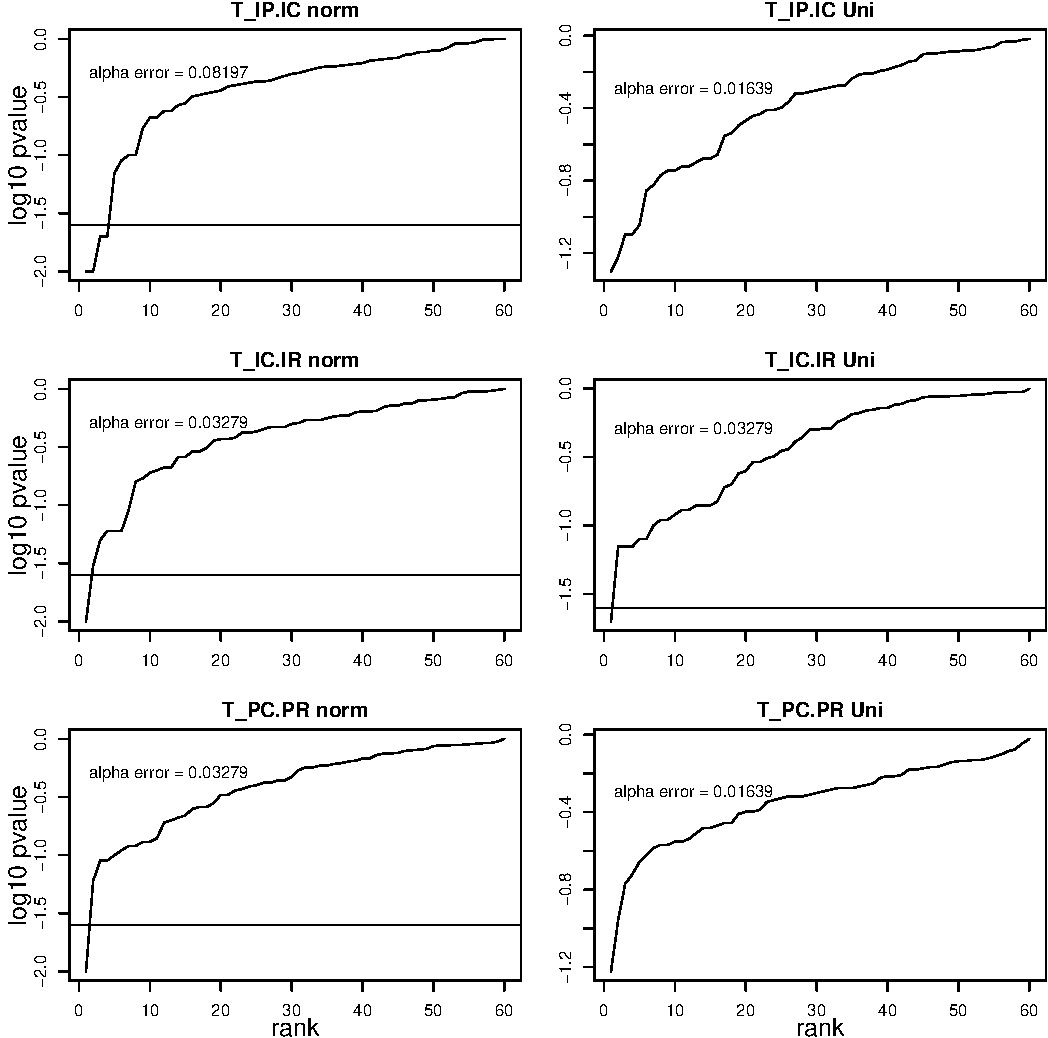
\includegraphics[width=\maxwidth]{figure/No_Filter_results-1} 

}

\caption[Local alpha errors]{Local alpha errors: local p.values are log-transformed and ordered before plotting. The black line represent the value of 0.025. Consequently, p-values under this line are false-positive cases. Alpha-error is the proportion of this false-positive cases. Norm: normal distribution, Uni: uniforme distribution.\label{fig:No_Filter_results}}
\end{figure}


\end{knitrout}

 \subsection {Assess the statistical type I error of global T-statistics}

In contrast with local p-values, we call global p-values the p-values corresponding to one indice for one trait across all the communities. 

We test for the \textbf{alpha error} of global p-values in the same way as local p-values. We plot the ordered mean \footnote{mean of the ten communities values} standardized effect size (SES)\foonote{compute as $(the observed value - the mean value among simulation) / the standard error among simulations$} and the 95\% confidence interval in grey. 

In that case we have one p-value by T-statistics by traits for each of the 1000 permutations.

\begin{knitrout}\small
\definecolor{shadecolor}{rgb}{0.969, 0.969, 0.969}\color{fgcolor}\begin{kframe}
\begin{alltt}
\hlstd{meanSES.1.T_IP.IC.distriNorm} \hlkwb{<-} \hlkwd{lapply}\hlstd{(res.simu1,} \hlkwa{function}\hlstd{(}\hlkwc{x}\hlstd{)}
          \hlkwd{mean}\hlstd{(}\hlkwd{ses.listofindex}\hlstd{(}\hlkwd{as.listofindex}\hlstd{(x))}
           \hlopt{$}\hlstd{index_1_1}\hlopt{$}\hlstd{ses[,}\hlnum{1}\hlstd{],} \hlkwc{na.rm} \hlstd{= T))}

\hlstd{meanSES.1.T_IC.IR.distriNorm} \hlkwb{<-} \hlkwd{lapply}\hlstd{(res.simu1,} \hlkwa{function}\hlstd{(}\hlkwc{x}\hlstd{)}
          \hlkwd{mean}\hlstd{(}\hlkwd{ses.listofindex}\hlstd{(}\hlkwd{as.listofindex}\hlstd{(x))}
           \hlopt{$}\hlstd{index_1_2}\hlopt{$}\hlstd{ses[,}\hlnum{1}\hlstd{],} \hlkwc{na.rm} \hlstd{= T))}

\hlstd{meanSES.1.T_PC.PR.distriNorm} \hlkwb{<-} \hlkwd{lapply}\hlstd{(res.simu1,} \hlkwa{function}\hlstd{(}\hlkwc{x}\hlstd{)}
          \hlkwd{mean}\hlstd{(}\hlkwd{ses.listofindex}\hlstd{(}\hlkwd{as.listofindex}\hlstd{(x))}
           \hlopt{$}\hlstd{index_1_3}\hlopt{$}\hlstd{ses[,}\hlnum{1}\hlstd{],} \hlkwc{na.rm} \hlstd{= T))}

\hlstd{meanSES.1.T_IP.IC.distriUni} \hlkwb{<-} \hlkwd{lapply}\hlstd{(res.simu1,} \hlkwa{function}\hlstd{(}\hlkwc{x}\hlstd{)}
          \hlkwd{mean}\hlstd{(}\hlkwd{ses.listofindex}\hlstd{(}\hlkwd{as.listofindex}\hlstd{(x))}
           \hlopt{$}\hlstd{index_1_1}\hlopt{$}\hlstd{ses[,}\hlnum{2}\hlstd{],} \hlkwc{na.rm} \hlstd{= T))}

\hlstd{meanSES.1.T_IC.IR.distriUni} \hlkwb{<-} \hlkwd{lapply}\hlstd{(res.simu1,} \hlkwa{function}\hlstd{(}\hlkwc{x}\hlstd{)}
          \hlkwd{mean}\hlstd{(}\hlkwd{ses.listofindex}\hlstd{(}\hlkwd{as.listofindex}\hlstd{(x))}\hlopt{$}
            \hlstd{index_1_2}\hlopt{$}\hlstd{ses[,}\hlnum{2}\hlstd{],} \hlkwc{na.rm} \hlstd{= T))}

\hlstd{meanSES.1.T_PC.PR.distriUni} \hlkwb{<-} \hlkwd{lapply}\hlstd{(res.simu1,} \hlkwa{function}\hlstd{(}\hlkwc{x}\hlstd{)}
          \hlkwd{mean}\hlstd{(}\hlkwd{ses.listofindex}\hlstd{(}\hlkwd{as.listofindex}\hlstd{(x))}
           \hlopt{$}\hlstd{index_1_3}\hlopt{$}\hlstd{ses[,}\hlnum{2}\hlstd{],} \hlkwc{na.rm} \hlstd{= T))}
\end{alltt}
\end{kframe}
\end{knitrout}

Now, plot the result as ordered SES values (Fig. \ref{fig:No_filter_summary_plot}). Horizontal lines represent the confidence area at 95\%.
 
\begin{knitrout}\small
\definecolor{shadecolor}{rgb}{0.969, 0.969, 0.969}\color{fgcolor}\begin{kframe}
\begin{alltt}
\hlkwd{par}\hlstd{(}\hlkwc{mfrow} \hlstd{=} \hlkwd{c}\hlstd{(}\hlnum{3}\hlstd{,} \hlnum{2}\hlstd{))}
\hlkwd{par}\hlstd{(}\hlkwc{mar} \hlstd{=} \hlkwd{c}\hlstd{(}\hlnum{3}\hlstd{,} \hlnum{3.5}\hlstd{,} \hlnum{2}\hlstd{,} \hlnum{0.2}\hlstd{))}

\hlcom{####   T_IP.IC}
\hlcom{#T_IP.IC.distriNorm}
\hlstd{xx} \hlkwb{<-} \hlkwd{sort}\hlstd{(}\hlkwd{unlist}\hlstd{(meanSES.1.T_IP.IC.distriNorm))}
\hlstd{xx_lim.inf} \hlkwb{<-} \hlkwd{unlist}\hlstd{(}\hlkwd{lapply}\hlstd{(res.simu1,} \hlkwa{function}\hlstd{(}\hlkwc{x}\hlstd{)} \hlkwd{mean}\hlstd{(}\hlkwd{ses.listofindex}\hlstd{(}\hlkwd{as.listofindex}\hlstd{(x))}
              \hlopt{$}\hlstd{index_1_1}\hlopt{$}\hlstd{ses.inf[,}\hlnum{1}\hlstd{],} \hlkwc{na.rm} \hlstd{= T)))}
\hlstd{xx_lim.sup} \hlkwb{<-} \hlkwd{unlist}\hlstd{(}\hlkwd{lapply}\hlstd{(res.simu1,} \hlkwa{function}\hlstd{(}\hlkwc{x}\hlstd{)} \hlkwd{mean}\hlstd{(}\hlkwd{ses.listofindex}\hlstd{(}\hlkwd{as.listofindex}\hlstd{(x))}
              \hlopt{$}\hlstd{index_1_1}\hlopt{$}\hlstd{ses.sup[,}\hlnum{1}\hlstd{],} \hlkwc{na.rm} \hlstd{= T)))}
\hlstd{alpha1} \hlkwb{<-} \hlkwd{round}\hlstd{((}\hlkwd{sum}\hlstd{(xx}\hlopt{<}\hlstd{xx_lim.inf} \hlopt{|} \hlstd{xx}\hlopt{>}\hlstd{xx_lim.sup)}\hlopt{+}\hlnum{1}\hlstd{)} \hlopt{/} \hlstd{(}\hlkwd{length}\hlstd{(xx)}\hlopt{+}\hlnum{1}\hlstd{),} \hlnum{3}\hlstd{)}

\hlkwd{plot}\hlstd{(xx,} \hlkwc{type} \hlstd{=} \hlstr{"l"}\hlstd{,} \hlkwc{main} \hlstd{=} \hlstr{"T_IP.IC norm"}\hlstd{,} \hlkwc{ylim} \hlstd{=} \hlkwd{c}\hlstd{(}\hlopt{-}\hlnum{3}\hlstd{,} \hlnum{3}\hlstd{),}
     \hlkwc{ylab} \hlstd{=} \hlnum{NA}\hlstd{,} \hlkwc{xlab} \hlstd{=} \hlnum{NA}\hlstd{)}
\hlkwd{rect}\hlstd{(}\hlopt{-}\hlnum{100}\hlstd{,} \hlkwd{mean}\hlstd{(xx_lim.inf), npermut}\hlopt{*}\hlnum{1.2}\hlstd{,} \hlkwd{mean}\hlstd{(xx_lim.sup),} \hlkwc{col} \hlstd{=} \hlkwd{rgb}\hlstd{(}\hlnum{0}\hlstd{,} \hlnum{0}\hlstd{,} \hlnum{0}\hlstd{,} \hlnum{0.2}\hlstd{))}
\hlkwd{text}\hlstd{(}\hlnum{3}\hlstd{,} \hlnum{0.8}\hlstd{,} \hlkwc{labels} \hlstd{=} \hlkwd{paste}\hlstd{(}\hlstr{"alpha error"}\hlstd{, alpha1,} \hlkwc{sep} \hlstd{=} \hlstr{" = "}\hlstd{),} \hlkwc{cex} \hlstd{=} \hlnum{0.7}\hlstd{,} \hlkwc{pos} \hlstd{=} \hlnum{4}\hlstd{)}
\hlkwd{mtext}\hlstd{(}\hlstr{"Standardized Effect Size"}\hlstd{,} \hlnum{2}\hlstd{,} \hlkwc{line} \hlstd{=} \hlnum{2}\hlstd{)}

\hlcom{#T_IP.IC.distriUni}
\hlstd{xx} \hlkwb{<-} \hlkwd{sort}\hlstd{(}\hlkwd{unlist}\hlstd{(meanSES.1.T_IP.IC.distriUni))}
\hlstd{xx_lim.inf} \hlkwb{<-} \hlkwd{unlist}\hlstd{(}\hlkwd{lapply}\hlstd{(res.simu1,} \hlkwa{function}\hlstd{(}\hlkwc{x}\hlstd{)} \hlkwd{mean}\hlstd{(}\hlkwd{ses.listofindex}\hlstd{(}\hlkwd{as.listofindex}\hlstd{(x))}
              \hlopt{$}\hlstd{index_1_1}\hlopt{$}\hlstd{ses.inf[,}\hlnum{2}\hlstd{],} \hlkwc{na.rm} \hlstd{= T)))}
\hlstd{xx_lim.sup} \hlkwb{<-} \hlkwd{unlist}\hlstd{(}\hlkwd{lapply}\hlstd{(res.simu1,} \hlkwa{function}\hlstd{(}\hlkwc{x}\hlstd{)} \hlkwd{mean}\hlstd{(}\hlkwd{ses.listofindex}\hlstd{(}\hlkwd{as.listofindex}\hlstd{(x))}
              \hlopt{$}\hlstd{index_1_1}\hlopt{$}\hlstd{ses.sup[,}\hlnum{2}\hlstd{],} \hlkwc{na.rm} \hlstd{= T)))}
\hlstd{alpha2} \hlkwb{<-} \hlkwd{round}\hlstd{((}\hlkwd{sum}\hlstd{(xx}\hlopt{<}\hlstd{xx_lim.inf} \hlopt{|} \hlstd{xx}\hlopt{>}\hlstd{xx_lim.sup)}\hlopt{+}\hlnum{1}\hlstd{)} \hlopt{/} \hlstd{(}\hlkwd{length}\hlstd{(xx)}\hlopt{+}\hlnum{1}\hlstd{),} \hlnum{3}\hlstd{)}

\hlkwd{plot}\hlstd{(xx,} \hlkwc{type} \hlstd{=} \hlstr{"l"}\hlstd{,} \hlkwc{main} \hlstd{=} \hlstr{"T_IP.IC uni"}\hlstd{,} \hlkwc{ylim} \hlstd{=} \hlkwd{c}\hlstd{(}\hlopt{-}\hlnum{3}\hlstd{,} \hlnum{3}\hlstd{),}
     \hlkwc{ylab} \hlstd{=} \hlnum{NA}\hlstd{,} \hlkwc{xlab} \hlstd{=} \hlnum{NA}\hlstd{)}
\hlkwd{rect}\hlstd{(}\hlopt{-}\hlnum{100}\hlstd{,} \hlkwd{mean}\hlstd{(xx_lim.inf), npermut}\hlopt{*}\hlnum{1.2}\hlstd{,} \hlkwd{mean}\hlstd{(xx_lim.sup),} \hlkwc{col} \hlstd{=} \hlkwd{rgb}\hlstd{(}\hlnum{0}\hlstd{,} \hlnum{0}\hlstd{,} \hlnum{0}\hlstd{,} \hlnum{0.2}\hlstd{))}
\hlkwd{text}\hlstd{(}\hlnum{3}\hlstd{,} \hlnum{0.8}\hlstd{,} \hlkwc{labels} \hlstd{=} \hlkwd{paste}\hlstd{(}\hlstr{"alpha error"}\hlstd{, alpha2,} \hlkwc{sep} \hlstd{=} \hlstr{" = "}\hlstd{),} \hlkwc{cex} \hlstd{=} \hlnum{0.7}\hlstd{,} \hlkwc{pos} \hlstd{=} \hlnum{4}\hlstd{)}

\hlcom{#__________}
\hlcom{####   T_IC.IR}
\hlcom{#T_IC.IR.distriNorm}
\hlstd{xx} \hlkwb{<-} \hlkwd{sort}\hlstd{(}\hlkwd{unlist}\hlstd{(meanSES.1.T_IC.IR.distriNorm))}

\hlstd{xx_lim.inf} \hlkwb{<-} \hlkwd{unlist}\hlstd{(}\hlkwd{lapply}\hlstd{(res.simu1,} \hlkwa{function}\hlstd{(}\hlkwc{x}\hlstd{)} \hlkwd{mean}\hlstd{(}\hlkwd{ses.listofindex}\hlstd{(}\hlkwd{as.listofindex}\hlstd{(x))}
              \hlopt{$}\hlstd{index_1_2}\hlopt{$}\hlstd{ses.inf[,}\hlnum{1}\hlstd{],} \hlkwc{na.rm} \hlstd{= T)))}
\hlstd{xx_lim.sup} \hlkwb{<-} \hlkwd{unlist}\hlstd{(}\hlkwd{lapply}\hlstd{(res.simu1,} \hlkwa{function}\hlstd{(}\hlkwc{x}\hlstd{)} \hlkwd{mean}\hlstd{(}\hlkwd{ses.listofindex}\hlstd{(}\hlkwd{as.listofindex}\hlstd{(x))}
              \hlopt{$}\hlstd{index_1_2}\hlopt{$}\hlstd{ses.sup[,}\hlnum{1}\hlstd{],} \hlkwc{na.rm} \hlstd{= T)))}
\hlstd{alpha3} \hlkwb{<-} \hlkwd{round}\hlstd{((}\hlkwd{sum}\hlstd{(xx}\hlopt{<}\hlstd{xx_lim.inf} \hlopt{|} \hlstd{xx}\hlopt{>}\hlstd{xx_lim.sup)}\hlopt{+}\hlnum{1}\hlstd{)} \hlopt{/} \hlstd{(}\hlkwd{length}\hlstd{(xx)}\hlopt{+}\hlnum{1}\hlstd{),} \hlnum{3}\hlstd{)}

\hlkwd{plot}\hlstd{(xx,} \hlkwc{type} \hlstd{=} \hlstr{"l"}\hlstd{,} \hlkwc{main} \hlstd{=} \hlstr{"T_IC.IR norm"}\hlstd{,} \hlkwc{ylim} \hlstd{=} \hlkwd{c}\hlstd{(}\hlopt{-}\hlnum{3}\hlstd{,} \hlnum{3}\hlstd{),}
     \hlkwc{ylab} \hlstd{=} \hlnum{NA}\hlstd{,} \hlkwc{xlab} \hlstd{=} \hlnum{NA}\hlstd{)}
\hlkwd{rect}\hlstd{(}\hlopt{-}\hlnum{100}\hlstd{,} \hlkwd{mean}\hlstd{(xx_lim.inf), npermut}\hlopt{*}\hlnum{1.2}\hlstd{,} \hlkwd{mean}\hlstd{(xx_lim.sup),} \hlkwc{col} \hlstd{=} \hlkwd{rgb}\hlstd{(}\hlnum{0}\hlstd{,} \hlnum{0}\hlstd{,} \hlnum{0}\hlstd{,} \hlnum{0.2}\hlstd{))}
\hlkwd{text}\hlstd{(}\hlnum{3}\hlstd{,} \hlnum{0.8}\hlstd{,} \hlkwc{labels} \hlstd{=} \hlkwd{paste}\hlstd{(}\hlstr{"alpha error"}\hlstd{, alpha3,} \hlkwc{sep} \hlstd{=} \hlstr{" = "}\hlstd{),} \hlkwc{cex} \hlstd{=} \hlnum{0.7}\hlstd{,} \hlkwc{pos} \hlstd{=} \hlnum{4}\hlstd{)}
\hlkwd{mtext}\hlstd{(}\hlstr{"Standardized Effect Size"}\hlstd{,} \hlnum{2}\hlstd{,} \hlkwc{line} \hlstd{=} \hlnum{2}\hlstd{)}

\hlcom{#T_IC.IR.distriUni}
\hlstd{xx} \hlkwb{<-} \hlkwd{sort}\hlstd{(}\hlkwd{unlist}\hlstd{(meanSES.1.T_IC.IR.distriUni))}

\hlstd{xx_lim.inf} \hlkwb{<-} \hlkwd{unlist}\hlstd{(}\hlkwd{lapply}\hlstd{(res.simu1,} \hlkwa{function}\hlstd{(}\hlkwc{x}\hlstd{)} \hlkwd{mean}\hlstd{(}\hlkwd{ses.listofindex}\hlstd{(}\hlkwd{as.listofindex}\hlstd{(x))}
              \hlopt{$}\hlstd{index_1_2}\hlopt{$}\hlstd{ses.inf[,}\hlnum{2}\hlstd{],} \hlkwc{na.rm} \hlstd{= T)))}
\hlstd{xx_lim.sup} \hlkwb{<-} \hlkwd{unlist}\hlstd{(}\hlkwd{lapply}\hlstd{(res.simu1,} \hlkwa{function}\hlstd{(}\hlkwc{x}\hlstd{)} \hlkwd{mean}\hlstd{(}\hlkwd{ses.listofindex}\hlstd{(}\hlkwd{as.listofindex}\hlstd{(x))}
              \hlopt{$}\hlstd{index_1_2}\hlopt{$}\hlstd{ses.sup[,}\hlnum{2}\hlstd{],} \hlkwc{na.rm} \hlstd{= T)))}
\hlstd{alpha4} \hlkwb{<-} \hlkwd{round}\hlstd{((}\hlkwd{sum}\hlstd{(xx}\hlopt{<}\hlstd{xx_lim.inf} \hlopt{|} \hlstd{xx}\hlopt{>}\hlstd{xx_lim.sup)}\hlopt{+}\hlnum{1}\hlstd{)} \hlopt{/} \hlstd{(}\hlkwd{length}\hlstd{(xx)}\hlopt{+}\hlnum{1}\hlstd{),} \hlnum{3}\hlstd{)}

\hlkwd{plot}\hlstd{(xx,} \hlkwc{type} \hlstd{=} \hlstr{"l"}\hlstd{,} \hlkwc{main} \hlstd{=} \hlstr{"T_IC.IR uni"}\hlstd{,} \hlkwc{ylim} \hlstd{=} \hlkwd{c}\hlstd{(}\hlopt{-}\hlnum{3}\hlstd{,} \hlnum{3}\hlstd{),}
     \hlkwc{ylab} \hlstd{=} \hlnum{NA}\hlstd{,} \hlkwc{xlab} \hlstd{=} \hlnum{NA}\hlstd{)}
\hlkwd{rect}\hlstd{(}\hlopt{-}\hlnum{100}\hlstd{,} \hlkwd{mean}\hlstd{(xx_lim.inf), npermut}\hlopt{*}\hlnum{1.2}\hlstd{,} \hlkwd{mean}\hlstd{(xx_lim.sup),} \hlkwc{col} \hlstd{=} \hlkwd{rgb}\hlstd{(}\hlnum{0}\hlstd{,} \hlnum{0}\hlstd{,} \hlnum{0}\hlstd{,} \hlnum{0.2}\hlstd{))}
\hlkwd{text}\hlstd{(}\hlnum{3}\hlstd{,} \hlnum{0.8}\hlstd{,} \hlkwc{labels} \hlstd{=} \hlkwd{paste}\hlstd{(}\hlstr{"alpha error"}\hlstd{, alpha4,} \hlkwc{sep} \hlstd{=} \hlstr{" = "}\hlstd{),} \hlkwc{cex} \hlstd{=} \hlnum{0.7}\hlstd{,} \hlkwc{pos} \hlstd{=} \hlnum{4}\hlstd{)}

\hlcom{#__________}
\hlcom{####   T_PC.PR}
\hlcom{#T_PC.PR.distriNorm}
\hlstd{xx} \hlkwb{<-} \hlkwd{sort}\hlstd{(}\hlkwd{unlist}\hlstd{(meanSES.1.T_PC.PR.distriNorm))}

\hlstd{xx_lim.inf} \hlkwb{<-} \hlkwd{unlist}\hlstd{(}\hlkwd{lapply}\hlstd{(res.simu1,} \hlkwa{function}\hlstd{(}\hlkwc{x}\hlstd{)} \hlkwd{mean}\hlstd{(}\hlkwd{ses.listofindex}\hlstd{(}\hlkwd{as.listofindex}\hlstd{(x))}
              \hlopt{$}\hlstd{index_1_3}\hlopt{$}\hlstd{ses.inf[,}\hlnum{1}\hlstd{],} \hlkwc{na.rm} \hlstd{= T)))}
\hlstd{xx_lim.sup} \hlkwb{<-} \hlkwd{unlist}\hlstd{(}\hlkwd{lapply}\hlstd{(res.simu1,} \hlkwa{function}\hlstd{(}\hlkwc{x}\hlstd{)} \hlkwd{mean}\hlstd{(}\hlkwd{ses.listofindex}\hlstd{(}\hlkwd{as.listofindex}\hlstd{(x))}
              \hlopt{$}\hlstd{index_1_3}\hlopt{$}\hlstd{ses.sup[,}\hlnum{1}\hlstd{],} \hlkwc{na.rm} \hlstd{= T)))}
\hlstd{alpha5} \hlkwb{<-} \hlkwd{round}\hlstd{((}\hlkwd{sum}\hlstd{(xx}\hlopt{<}\hlstd{xx_lim.inf} \hlopt{|} \hlstd{xx}\hlopt{>}\hlstd{xx_lim.sup)}\hlopt{+}\hlnum{1}\hlstd{)} \hlopt{/} \hlstd{(}\hlkwd{length}\hlstd{(xx)}\hlopt{+}\hlnum{1}\hlstd{),} \hlnum{3}\hlstd{)}

\hlkwd{plot}\hlstd{(xx,} \hlkwc{type} \hlstd{=} \hlstr{"l"}\hlstd{,} \hlkwc{main} \hlstd{=} \hlstr{"T_PC.PR norm"}\hlstd{,} \hlkwc{ylim} \hlstd{=} \hlkwd{c}\hlstd{(}\hlopt{-}\hlnum{3}\hlstd{,} \hlnum{3}\hlstd{),}
     \hlkwc{ylab} \hlstd{=} \hlnum{NA}\hlstd{,} \hlkwc{xlab} \hlstd{=} \hlnum{NA}\hlstd{)}
\hlkwd{rect}\hlstd{(}\hlopt{-}\hlnum{100}\hlstd{,} \hlkwd{mean}\hlstd{(xx_lim.inf), npermut}\hlopt{*}\hlnum{1.2}\hlstd{,} \hlkwd{mean}\hlstd{(xx_lim.sup),} \hlkwc{col} \hlstd{=} \hlkwd{rgb}\hlstd{(}\hlnum{0}\hlstd{,} \hlnum{0}\hlstd{,} \hlnum{0}\hlstd{,} \hlnum{0.2}\hlstd{))}
\hlkwd{text}\hlstd{(}\hlnum{3}\hlstd{,} \hlnum{0.8}\hlstd{,} \hlkwc{labels} \hlstd{=} \hlkwd{paste}\hlstd{(}\hlstr{"alpha error"}\hlstd{, alpha5,} \hlkwc{sep} \hlstd{=} \hlstr{" = "}\hlstd{),} \hlkwc{cex} \hlstd{=} \hlnum{0.7}\hlstd{,} \hlkwc{pos} \hlstd{=} \hlnum{4}\hlstd{)}
\hlkwd{mtext}\hlstd{(}\hlstr{"Standardized Effect Size"}\hlstd{,} \hlnum{2}\hlstd{,} \hlkwc{line} \hlstd{=} \hlnum{2}\hlstd{)}
\hlkwd{mtext}\hlstd{(}\hlstr{"rank"}\hlstd{,} \hlnum{1}\hlstd{,} \hlkwc{line} \hlstd{=} \hlnum{2}\hlstd{)}

\hlcom{#T_PC.PR.distriUni}
\hlstd{xx} \hlkwb{<-} \hlkwd{sort}\hlstd{(}\hlkwd{unlist}\hlstd{(meanSES.1.T_PC.PR.distriUni))}
\hlstd{xx_lim.inf} \hlkwb{<-} \hlkwd{unlist}\hlstd{(}\hlkwd{lapply}\hlstd{(res.simu1,} \hlkwa{function}\hlstd{(}\hlkwc{x}\hlstd{)} \hlkwd{mean}\hlstd{(}\hlkwd{ses.listofindex}\hlstd{(}\hlkwd{as.listofindex}\hlstd{(x))}
              \hlopt{$}\hlstd{index_1_3}\hlopt{$}\hlstd{ses.inf[,}\hlnum{2}\hlstd{],} \hlkwc{na.rm} \hlstd{= T)))}
\hlstd{xx_lim.sup} \hlkwb{<-} \hlkwd{unlist}\hlstd{(}\hlkwd{lapply}\hlstd{(res.simu1,} \hlkwa{function}\hlstd{(}\hlkwc{x}\hlstd{)} \hlkwd{mean}\hlstd{(}\hlkwd{ses.listofindex}\hlstd{(}\hlkwd{as.listofindex}\hlstd{(x))}
              \hlopt{$}\hlstd{index_1_3}\hlopt{$}\hlstd{ses.sup[,}\hlnum{2}\hlstd{],} \hlkwc{na.rm} \hlstd{= T)))}
\hlstd{alpha6} \hlkwb{<-} \hlkwd{round}\hlstd{((}\hlkwd{sum}\hlstd{(xx}\hlopt{<}\hlstd{xx_lim.inf} \hlopt{|} \hlstd{xx}\hlopt{>}\hlstd{xx_lim.sup)}\hlopt{+}\hlnum{1}\hlstd{)} \hlopt{/} \hlstd{(}\hlkwd{length}\hlstd{(xx)}\hlopt{+}\hlnum{1}\hlstd{),} \hlnum{3}\hlstd{)}

\hlkwd{plot}\hlstd{(xx,} \hlkwc{type} \hlstd{=} \hlstr{"l"}\hlstd{,} \hlkwc{main} \hlstd{=} \hlstr{"T_PC.PR uni"}\hlstd{,} \hlkwc{ylim} \hlstd{=} \hlkwd{c}\hlstd{(}\hlopt{-}\hlnum{3}\hlstd{,} \hlnum{3}\hlstd{),}
     \hlkwc{ylab} \hlstd{=} \hlnum{NA}\hlstd{,} \hlkwc{xlab} \hlstd{=} \hlnum{NA}\hlstd{)}
\hlkwd{rect}\hlstd{(}\hlopt{-}\hlnum{100}\hlstd{,} \hlkwd{mean}\hlstd{(xx_lim.inf), npermut}\hlopt{*}\hlnum{1.2}\hlstd{,} \hlkwd{mean}\hlstd{(xx_lim.sup),} \hlkwc{col} \hlstd{=} \hlkwd{rgb}\hlstd{(}\hlnum{0}\hlstd{,} \hlnum{0}\hlstd{,} \hlnum{0}\hlstd{,} \hlnum{0.2}\hlstd{))}
\hlkwd{text}\hlstd{(}\hlnum{3}\hlstd{,} \hlnum{0.8}\hlstd{,} \hlkwc{labels} \hlstd{=} \hlkwd{paste}\hlstd{(}\hlstr{"alpha error"}\hlstd{, alpha6,} \hlkwc{sep} \hlstd{=} \hlstr{" = "}\hlstd{),} \hlkwc{cex} \hlstd{=} \hlnum{0.7}\hlstd{,} \hlkwc{pos} \hlstd{=} \hlnum{4}\hlstd{)}
\hlkwd{mtext}\hlstd{(}\hlstr{"rank"}\hlstd{,} \hlnum{1}\hlstd{,} \hlkwc{line} \hlstd{=} \hlnum{2}\hlstd{)}

\hlkwd{par}\hlstd{(oldpar)}
\end{alltt}
\end{kframe}\begin{figure}

{\centering 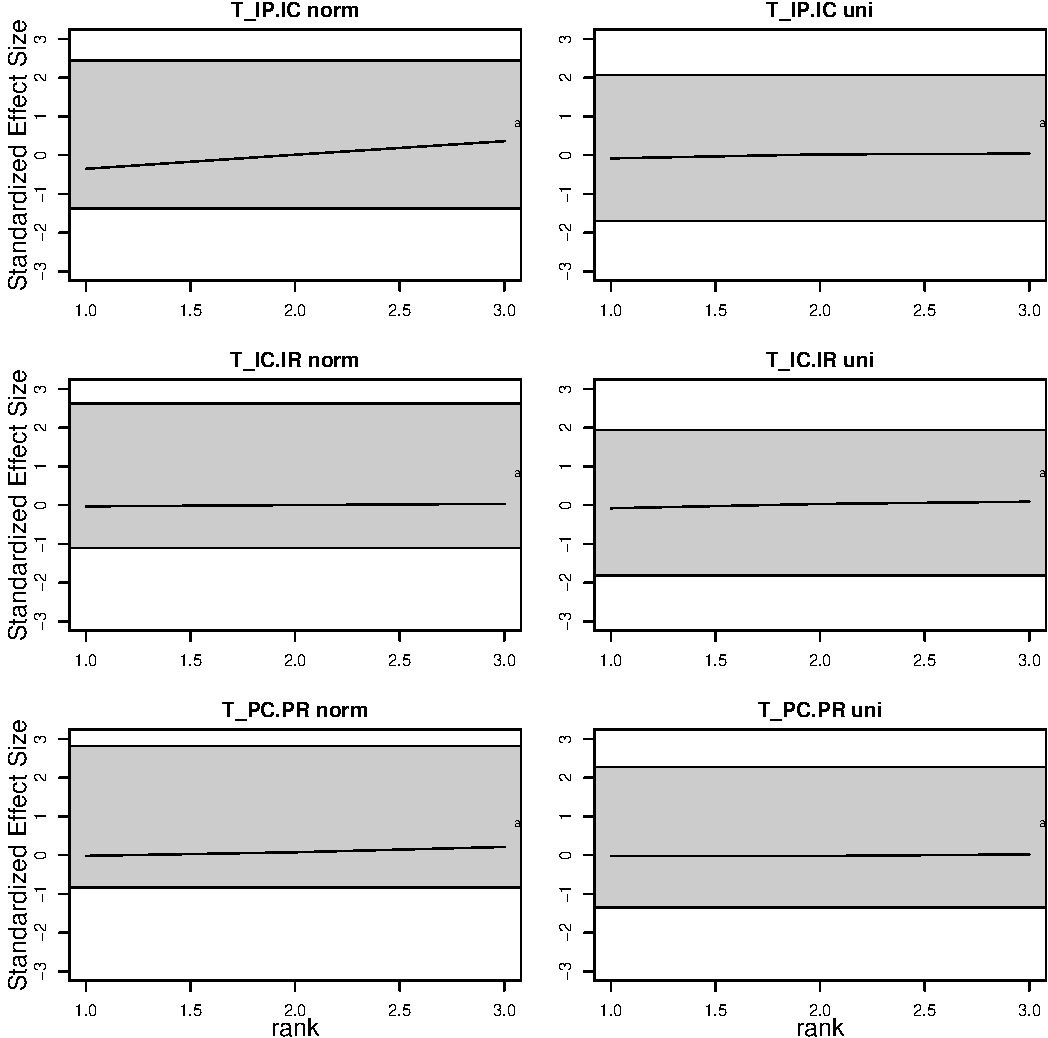
\includegraphics[width=\maxwidth]{figure/No_filter_summary_plot-1} 

}

\caption[Global alpha errors]{Global alpha errors: global Standardized Effect Size are ordered before plotting. The grey area represent the confidence interval at 2.5 percent on each side. Consequently, p-values outside this area are false-positive cases. Alpha-error is the proportion of this false-positive cases. Norm: normal distribution, Uni: uniforme distribution.\label{fig:No_filter_summary_plot}}
\end{figure}


\end{knitrout}

  \subsection {Conclusion on the type I error of T-statistics}

The 1000 permutations allow the calculation of alpha error for two traits (the first normally distributed and the second uniformally distributed), three indices (the three T-statistics) and using local indices (one by community) or global indices (averaged between communities).

\begin{table}[h!]
\begin{center}
\caption{Alpha-errors for T-statistics}
\label{tab:Alpha-errors_for_T-stats}
\begin{tabular}{|c|c|c|c|c|}
\hline
Traits & Indices & Average between communities? & alpha-error \tabularnewline
\hline \hline \hline
\multirow{6}{*}{Trait normally distributed} & \multirow{2}{*}{$T_{IP/IC}$} & no (local) & 0.026 \tabularnewline
\cline{3-4} 
 & & yes (global) & 0.001 \tabularnewline
\cline{2-4} 
 & \multirow{2}{*}{$T_{IC/IR}$} & no (local) & 0.02 \tabularnewline
\cline{3-4} 
 & & yes (global) & 0.001 \tabularnewline
\cline{2-4} 
 & \multirow{2}{*}{$T_{PC/PR}$} & no (local) & 0.04 \tabularnewline
\cline{3-4}
 & & yes (global)& 0.001 \tabularnewline

\hline \hline \hline

\multirow{6}{*}{Trait uniformally distributed} & \multirow{2}{*}{$T_{IP/IC}$} & no (local) & 0.02 \tabularnewline
\cline{3-4}
 & & yes (global) &  0.001 \tabularnewline
\cline{2-4} 
 & \multirow{2}{*}{$T_{IC/IR}$} & no (local) & 0.02 \tabularnewline
\cline{3-4} 
 & & yes (global) &  0.001 \tabularnewline
\cline{2-4} 
 & \multirow{2}{*}{$T_{PC/PR}$} & no (local) & 0.006 \tabularnewline
\cline{3-4} 
 & & yes (global)&  0.001 \tabularnewline
\hline 
\end{tabular}
\end{center}
\end{table}



The results of table \ref{tab:Alpha-errors_for_T-stats} attest of a good behavior of the T-statistics regardless of the distributions of the traits. Alpha-error of the local indices are always near the wanted alpha-error of 2.5\%. Logically the global indices which averaged local indices are far more robust. Note that the higher alpha-error is obtain using $T_{PC/PR}$ on the trait normally distributed (0.04).















































\cleardoublepage

\section{Internal filter: assess the statistical power of $T_{IP/IC}$}
  \subsection {Randomization outline}
 
We decide to modulate the strength of the internal filter thanks to two parameters:
we define (i) a gradient of distance between species means traits distributions and (ii) a gradient of the mean variance in species traits distributions. It is strongly link to the definition of limiting similarity by May and Mac Arthur (1972) who defined a coefficient of competition as $$a = exp (-d^2/4w^2)$$ with \texttt{d} correspond to the distance between the species trait means and \texttt{w} correspond to the mean variance of species trait distribution. 

\begin{knitrout}\small
\definecolor{shadecolor}{rgb}{0.969, 0.969, 0.969}\color{fgcolor}\begin{kframe}
\begin{alltt}
\hlcom{# Number of values for each parameters: param_DIST_between_MEAN.init and param_SD}
\hlstd{nb_param_val}
\end{alltt}
\begin{verbatim}
## [1] 10
\end{verbatim}
\begin{alltt}
\hlcom{# Number of permutations is the product of the number of values for each parameter}
\hlcom{#(nb_param_val) and the number of permutations by parameter (N_repet_Param)}
\hlstd{nperm} \hlkwb{<-} \hlstd{nb_param_val} \hlopt{*} \hlstd{N_repet_Param}

\hlcom{# Maximum mean value for traits}
\hlstd{max.value_traits} \hlkwb{<-} \hlnum{250}

\hlcom{# Parameter for the distance between species mean trait values}
\hlstd{param_DIST_between_MEAN.init} \hlkwb{<-} \hlkwd{round}\hlstd{(}\hlkwd{sort}\hlstd{(}\hlkwd{seq}\hlstd{(}\hlnum{10}\hlstd{,} \hlnum{200}\hlstd{,} \hlkwc{length.out} \hlstd{= nb_param_val)),} \hlnum{2}\hlstd{)}
\hlstd{param_DIST_between_MEAN} \hlkwb{<-} \hlkwd{rep}\hlstd{(param_DIST_between_MEAN.init, N_repet_Param)}
\hlstd{mean_sd.param} \hlkwb{<-} \hlkwd{rep}\hlstd{(}\hlnum{10}\hlstd{, nperm)}

\hlcom{# Parameter for the variance in species mean trait values}
\hlstd{param_SD} \hlkwb{<-} \hlkwd{seq}\hlstd{(}\hlnum{10}\hlstd{,} \hlnum{100}\hlstd{,}\hlkwc{length.out} \hlstd{= nb_param_val)}
\hlstd{sd_mean.param} \hlkwb{<-} \hlkwd{sample} \hlstd{(}\hlkwd{rep}\hlstd{(param_SD, N_repet_Param),}
       \hlkwc{size} \hlstd{=} \hlkwd{length}\hlstd{(}\hlkwd{rep}\hlstd{(param_SD, N_repet_Param)),} \hlkwc{replace} \hlstd{= F)}
\hlstd{sd_sd.param} \hlkwb{<-} \hlkwd{rep}\hlstd{(}\hlnum{10}\hlstd{, nperm)}
\end{alltt}
\end{kframe}
\end{knitrout}


 Practically, we defined 10 values for two parameters:
\\

 (i) \texttt{param\_{}DIST\_{}between\_{}MEAN.init} is a vector of length 10 which defined the minimum values for the mean traits values (the maximum values are defined to 250). In decreasing the range of traits values while keeping the same number of species, there is a decrease of mean distance between species means of traits values. Thus the mean for each species is drawing from a normal distribution with standard deviation of 10 (parameter \texttt{mean\_{}sd.param}) and means evenly distributed between \texttt{max.value\_{}traits - param\_{}DIST\_{}between\_{}MEAN} and \texttt{max.value\_{}traits}.
\\

(ii) \texttt{param\_{}SD} is a vector of length 10 which defined the standard deviation of traits distributions for each species. In order to decorrelating the mean and standard deviation of species traits distributions, \texttt{param\_{}SD} is sample before the analysis. 
\\

For the trait "a" the trait value for each individual is drawing from a normal distribution with the mean depending of it species attribute. For the trait "b" the trait value for each individual is drawing from a uniform distribution with the range depending of it species attribute. The range is defined as: \textit{species mean value} - \textit{species sd value} for the minimum and \textit{species mean value} + \textit{species sd value} for the maximum.

Now we can start the simulation of 10 parameters values and 2000 permutations. 

\begin{knitrout}\small
\definecolor{shadecolor}{rgb}{0.969, 0.969, 0.969}\color{fgcolor}\begin{kframe}
\begin{alltt}
\hlstd{mean.sp_stock2} \hlkwb{<-} \hlkwd{list}\hlstd{() ; sd.sp_stock2} \hlkwb{<-} \hlkwd{list}\hlstd{() ; res.simu2} \hlkwb{<-} \hlkwd{list}\hlstd{()}
\hlstd{res.simu2.pval} \hlkwb{<-} \hlkwd{list}\hlstd{() ; res.simu.traits2} \hlkwb{<-} \hlkwd{list}\hlstd{() ;  mean_dist_sp} \hlkwb{<-} \hlkwd{list}\hlstd{()}

\hlkwa{for}\hlstd{(n} \hlkwa{in} \hlnum{1}\hlopt{:}\hlstd{nperm)\{}\hlcom{#for each permutation}

 \hlcom{# Draw communities using lognormal distribution of abondances }
 \hlcom{# 100 individuals by populations}
 \hlstd{ex.sp2} \hlkwb{<-} \hlkwd{c}\hlstd{()}
 \hlstd{ex.com2} \hlkwb{<-} \hlkwd{matrix}\hlstd{(}\hlnum{0}\hlstd{,} \hlkwc{nrow} \hlstd{= Ncom,} \hlkwc{ncol} \hlstd{= Nsp)}
 \hlkwa{for}\hlstd{(i} \hlkwa{in} \hlnum{1}\hlopt{:} \hlstd{Ncom)\{}
  \hlstd{ex.com.interm} \hlkwb{<-} \hlkwd{table}\hlstd{(}\hlkwd{sample}\hlstd{(sp,} \hlkwc{size} \hlstd{= Nind}\hlopt{/}\hlstd{Ncom,} \hlkwc{prob} \hlstd{=} \hlkwd{rlnorm}\hlstd{(Nsp,} \hlnum{0}\hlstd{, sdlog),}
                                \hlkwc{replace} \hlstd{= T))}
  \hlstd{ex.com2[i, sp}\hlopt \hlkwd{names}\hlstd{(ex.com.interm)]} \hlkwb{<-} \hlstd{ex.com.interm}
  \hlstd{ex.sp2} \hlkwb{<-} \hlkwd{c}\hlstd{(ex.sp2,} \hlkwd{rep}\hlstd{(sp,} \hlkwc{times} \hlstd{= ex.com2[i,]))}
 \hlstd{\}}

 \hlstd{ex.indplot2} \hlkwb{<-} \hlkwd{as.factor}\hlstd{(}\hlkwd{rep}\hlstd{(com, Nind}\hlopt{/}\hlstd{Ncom))}

 \hlcom{# Defining traits mean and sd by species }
 \hlstd{mean_mean.param.interm} \hlkwb{<-} \hlkwd{seq}\hlstd{(max.value_traits} \hlopt{-} \hlstd{param_DIST_between_MEAN[n],}
                               \hlstd{max.value_traits,} \hlkwc{length.out} \hlstd{=}
                               \hlkwd{length}\hlstd{(}\hlkwd{unique}\hlstd{(param_DIST_between_MEAN)))}

 \hlstd{mean_mean.param} \hlkwb{<-} \hlkwd{rep}\hlstd{(}\hlkwd{round}\hlstd{(}\hlkwd{sort}\hlstd{(mean_mean.param.interm),} \hlnum{2}\hlstd{), N_repet_Param)}

 \hlstd{mean.sp} \hlkwb{<-} \hlkwd{rnorm}\hlstd{(}\hlkwd{length}\hlstd{(}\hlkwd{unique}\hlstd{(sp)),} \hlkwc{mean} \hlstd{= mean_mean.param,} \hlkwc{sd} \hlstd{= mean_sd.param[n])}
 \hlstd{sd.sp} \hlkwb{<-} \hlkwd{rnorm}\hlstd{(}\hlkwd{length}\hlstd{(}\hlkwd{unique}\hlstd{(sp)),} \hlkwc{mean} \hlstd{= sd_mean.param[n],} \hlkwc{sd} \hlstd{= sd_sd.param[n])}

 \hlstd{ex.traits2} \hlkwb{<-} \hlkwd{array}\hlstd{(}\hlnum{NA}\hlstd{,} \hlkwc{dim} \hlstd{=} \hlkwd{c}\hlstd{(Nind,} \hlnum{2}\hlstd{))}
 \hlkwd{colnames}\hlstd{(ex.traits2)} \hlkwb{<-} \hlkwd{paste}\hlstd{(}\hlstr{"trait"}\hlstd{,} \hlkwd{c}\hlstd{(}\hlstr{"a"}\hlstd{,} \hlstr{"b"}\hlstd{),} \hlkwc{sep} \hlstd{=} \hlstr{" "}\hlstd{)}

 \hlcom{# Draw the individual traits depending on species attributes}
  \hlkwa{for}\hlstd{(s} \hlkwa{in} \hlkwd{unique}\hlstd{(ex.sp2))\{}
   \hlcom{#trait a : normal distribution}
   \hlstd{ex.traits2[ex.sp2} \hlopt{==} \hlstd{s,} \hlnum{1}\hlstd{]} \hlkwb{<-}
   \hlkwd{rnorm}\hlstd{(}\hlnum{5}\hlopt{*}\hlstd{Nind}\hlopt{/}\hlstd{Ncom,} \hlkwd{rep}\hlstd{(mean.sp[}\hlkwd{unique}\hlstd{(ex.sp2)} \hlopt{==} \hlstd{s],} \hlnum{5}\hlopt{*}\hlstd{Nind}\hlopt{/}\hlstd{Ncom),}
         \hlkwd{rep}\hlstd{(sd.sp[}\hlkwd{unique}\hlstd{(ex.sp2)} \hlopt{==} \hlstd{s],} \hlnum{5}\hlopt{*}\hlstd{Nind}\hlopt{/}\hlstd{Ncom))[}\hlnum{1}\hlopt{:}\hlkwd{sum}\hlstd{(ex.sp2} \hlopt{==} \hlstd{s)]}

   \hlcom{#trait b : uniform distribution}
   \hlstd{ex.traits2[ex.sp2} \hlopt{==} \hlstd{s,} \hlnum{2}\hlstd{]} \hlkwb{<-}
   \hlkwd{runif}\hlstd{(}\hlnum{5}\hlopt{*}\hlstd{Nind}\hlopt{/}\hlstd{Ncom,} \hlkwc{min} \hlstd{=} \hlkwd{rep}\hlstd{(mean.sp[}\hlkwd{unique}\hlstd{(ex.sp2)} \hlopt{==} \hlstd{s],} \hlnum{5}\hlopt{*}\hlstd{Nind}\hlopt{/}\hlstd{Ncom)} \hlopt{-}
         \hlkwd{rep}\hlstd{(sd.sp[}\hlkwd{unique}\hlstd{(ex.sp2)} \hlopt{==} \hlstd{s],} \hlnum{5}\hlopt{*}\hlstd{Nind}\hlopt{/}\hlstd{Ncom),}
         \hlkwc{max} \hlstd{=} \hlkwd{rep}\hlstd{(mean.sp[}\hlkwd{unique}\hlstd{(ex.sp2)} \hlopt{==} \hlstd{s],} \hlnum{5}\hlopt{*}\hlstd{Nind}\hlopt{/}\hlstd{Ncom)} \hlopt{+}
         \hlkwd{rep}\hlstd{(sd.sp[}\hlkwd{unique}\hlstd{(ex.sp2)} \hlopt{==} \hlstd{s],} \hlnum{5}\hlopt{*}\hlstd{Nind}\hlopt{/}\hlstd{Ncom))[}\hlnum{1}\hlopt{:}\hlkwd{sum}\hlstd{(ex.sp2} \hlopt{==} \hlstd{s)]}
  \hlstd{\}}

 \hlcom{#stock results}
 \hlstd{mean.sp_stock2[[n]]} \hlkwb{<-} \hlstd{mean.sp}
 \hlstd{sd.sp_stock2[[n]]} \hlkwb{<-} \hlstd{sd.sp}

 \hlstd{mean_dist_sp[[n]]} \hlkwb{<-} \hlkwd{c}\hlstd{(}\hlkwd{mean}\hlstd{(}\hlkwd{tapply}\hlstd{(ex.traits2[,} \hlnum{1}\hlstd{], ex.indplot2,} \hlkwa{function}\hlstd{(}\hlkwc{x}\hlstd{)}
                                    \hlkwd{mean}\hlstd{(}\hlkwd{dist}\hlstd{(x),} \hlkwc{na.rm}\hlstd{=T)),} \hlkwc{na.rm}\hlstd{=T),}
                        \hlkwd{mean}\hlstd{(}\hlkwd{tapply}\hlstd{(ex.traits2[,} \hlnum{2}\hlstd{], ex.indplot2,} \hlkwa{function}\hlstd{(}\hlkwc{x}\hlstd{)}
                                    \hlkwd{mean}\hlstd{(}\hlkwd{dist}\hlstd{(x),} \hlkwc{na.rm}\hlstd{=T)),} \hlkwc{na.rm}\hlstd{=T))}

 \hlstd{res.simu.traits2[[n]]} \hlkwb{<-} \hlstd{ex.traits2}
 \hlstd{res.simu2[[n]]} \hlkwb{<-} \hlkwd{Tstats}\hlstd{(ex.traits2, ex.indplot2, ex.sp2,} \hlkwc{printprogress} \hlstd{=} \hlnum{FALSE}\hlstd{)}
 \hlstd{res.simu2.pval[[n]]} \hlkwb{<-} \hlkwd{sum_Tstats}\hlstd{(res.simu2[[n]],} \hlkwc{type} \hlstd{=} \hlstr{"p.value"}\hlstd{)}
 \hlkwd{print}\hlstd{(}\hlkwd{paste}\hlstd{(}\hlkwd{round}\hlstd{(n}\hlopt{/}\hlstd{nperm,} \hlnum{2}\hlstd{)} \hlopt{*} \hlstd{Nind}\hlopt{/}\hlstd{Ncom,} \hlstr{"%"}\hlstd{,} \hlkwc{sep} \hlstd{=} \hlstr{" "}\hlstd{))}
\hlstd{\}}\hlcom{#end of simulation}
\end{alltt}
\end{kframe}
\end{knitrout}


 \subsection {Results for simulations of internal filtering}

Let's see the result for one typical randomization. We can plot the distribution of traits within species and/or communities thanks to the function \texttt{plotDistri} (Fig. \ref{fig:typical_result_internal_filtering1}). 

\begin{knitrout}\small
\definecolor{shadecolor}{rgb}{0.969, 0.969, 0.969}\color{fgcolor}\begin{kframe}
\begin{alltt}
\hlkwd{par}\hlstd{(}\hlkwc{mfrow}\hlstd{=}\hlkwd{c}\hlstd{(}\hlnum{2}\hlstd{,} \hlnum{2}\hlstd{))}
\hlkwd{plotDistri}\hlstd{(ex.traits2,} \hlkwd{rep}\hlstd{(}\hlstr{"all_sp"}\hlstd{,} \hlkwc{times} \hlstd{=} \hlkwd{dim}\hlstd{(ex.traits2)[}\hlnum{1}\hlstd{]), ex.indplot2,}
           \hlkwc{plot.ask} \hlstd{= F,} \hlkwc{multipanel} \hlstd{= F,} \hlkwc{cex.leg} \hlstd{=} \hlnum{0.6}\hlstd{,} \hlkwc{main}\hlstd{=} \hlkwd{c}\hlstd{(}\hlstr{"a"}\hlstd{,} \hlstr{"b"}\hlstd{))}
\hlkwd{plotDistri}\hlstd{(ex.traits2,} \hlkwd{rep}\hlstd{(}\hlstr{"region"}\hlstd{,} \hlkwc{times} \hlstd{=} \hlkwd{dim}\hlstd{(ex.traits2)[}\hlnum{1}\hlstd{]), ex.sp2,} \hlkwc{plot.ask} \hlstd{= F,}
           \hlkwc{multipanel} \hlstd{= F,} \hlkwc{ylim} \hlstd{=} \hlkwd{c}\hlstd{(}\hlnum{0}\hlstd{,}\hlnum{0.04}\hlstd{),} \hlkwc{cex.leg} \hlstd{=} \hlnum{0.6}\hlstd{,} \hlkwc{main}\hlstd{=} \hlkwd{c}\hlstd{(}\hlstr{"c"}\hlstd{,} \hlstr{"d"}\hlstd{))}
\hlkwd{par}\hlstd{(}\hlkwc{mfrow}\hlstd{=}\hlkwd{c}\hlstd{(}\hlnum{1}\hlstd{,} \hlnum{1}\hlstd{))}
\end{alltt}
\end{kframe}\begin{figure}

{\centering 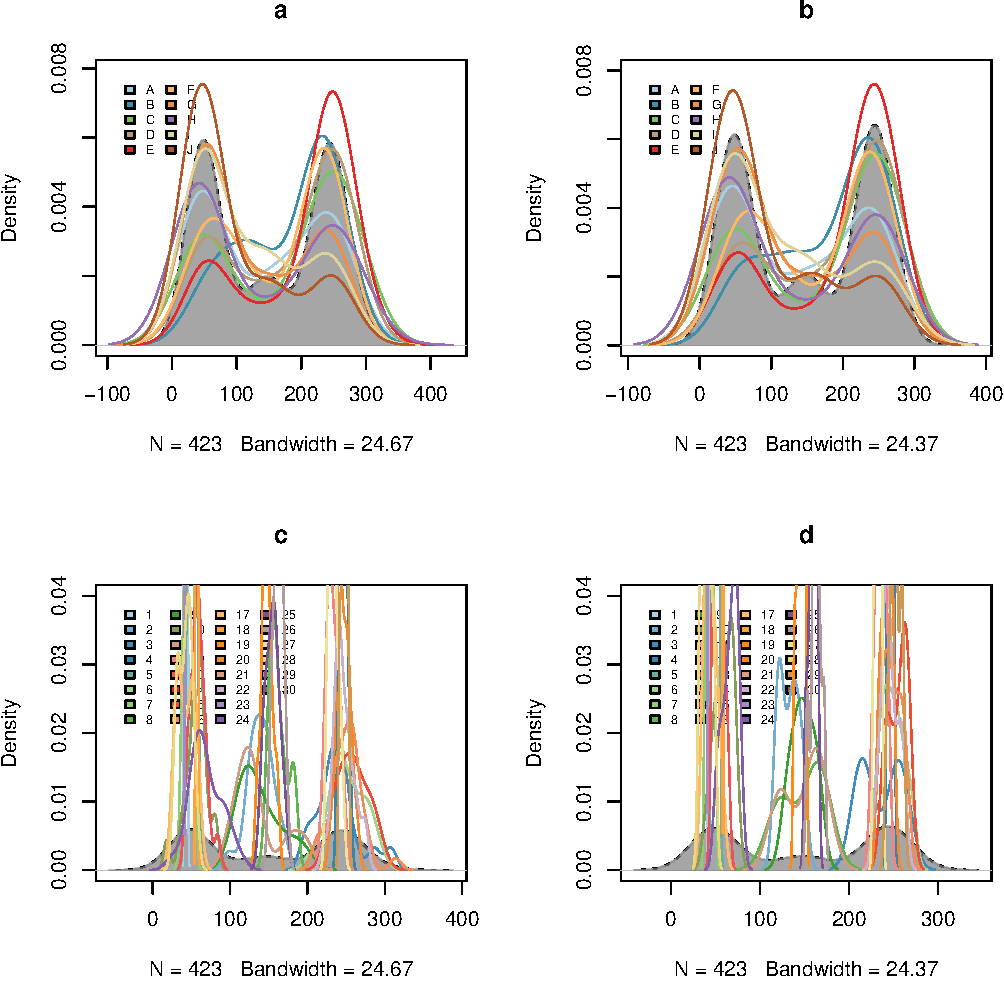
\includegraphics[width=\maxwidth]{figure/typical_result_internal_filtering1-1} 

}

\caption[Distribution of traits for one randomization with internal filtering]{Distribution of traits for one randomization with internal filtering: (a) Communities trait distributions for the trait a (normal distribution); (b) Communities trait distributions for the trait b (uniform distribution); (c) Species trait distributions for the trait a; (d) Species trait distributions for the trait b\label{fig:typical_result_internal_filtering1}}
\end{figure}


\end{knitrout}

We can also plot the result of the T-statistics for two contrasting cases (Fig. \ref{fig:typical_result_internal_filtering2}).

\begin{knitrout}\small
\definecolor{shadecolor}{rgb}{0.969, 0.969, 0.969}\color{fgcolor}\begin{kframe}
\begin{alltt}
\hlkwd{par}\hlstd{(}\hlkwc{mfrow}\hlstd{=}\hlkwd{c}\hlstd{(}\hlnum{2}\hlstd{,} \hlnum{1}\hlstd{))}
\hlkwd{plot}\hlstd{(res.simu2[[}\hlnum{1}\hlstd{]],} \hlkwc{main}\hlstd{=}\hlstr{"a"}\hlstd{)}
\hlkwd{plot}\hlstd{(res.simu2[[n]],} \hlkwc{main}\hlstd{=}\hlstr{"b"}\hlstd{)}
\hlkwd{par}\hlstd{(}\hlkwc{mfrow}\hlstd{=}\hlkwd{c}\hlstd{(}\hlnum{1}\hlstd{,} \hlnum{1}\hlstd{))}
\end{alltt}
\end{kframe}\begin{figure}

{\centering 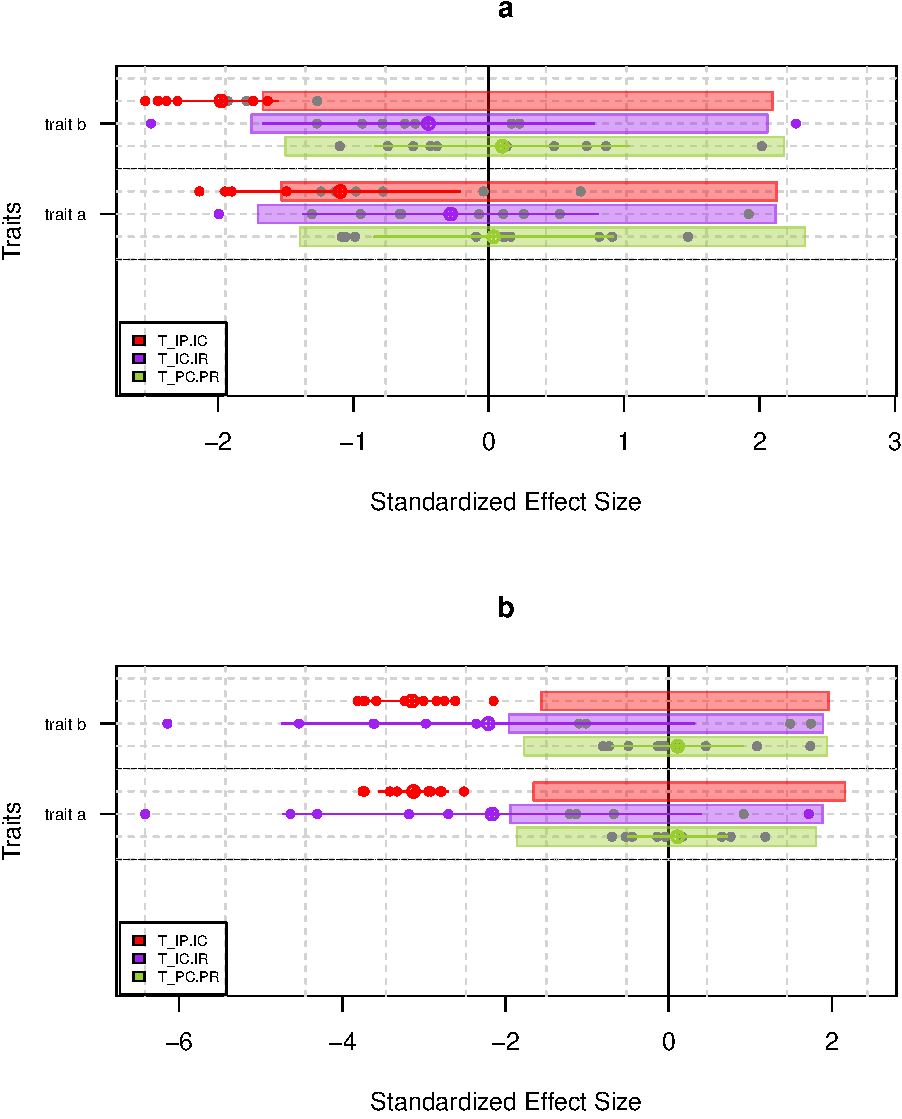
\includegraphics[width=\maxwidth]{figure/typical_result_internal_filtering2-1} 

}

\caption[Results of T-statistics for two randomization with contrasted strength of internal filtering]{Results of T-statistics for two randomization with contrasted strength of internal filtering: $T_{IP/IC}$ in red, $T_{IC/IR}$ in purple and $T_{PC/PR}$ in green. (a) Lower strength of internal filtering and (b) higher strength of internal filtering.\label{fig:typical_result_internal_filtering2}}
\end{figure}


\end{knitrout}

For the power analysis of internal filtering we present the result in two parts: (i) the test of robustness of each T-statistics values using local p-values and (ii) the test of community-aggregated T-statistics using global p-values.

 \subsubsection {Local p-values results}

Here we call local p-values the p-values corresponding to one indice for one trait in one community. First, we can represent the ordered p.value in decimal logarithms and calculate the power of the $T_{IP/IC}$ indice using the beta-error\footnote{The proportion of case where we do not reject the null hypothesis while this hypothesis is wrong.}. The less the beta-error, the more the indice is powerful. Contrary to the test with no filter, we choose a unilateral test because we only want to test if $T_{IP/IC}$ is smaller than it should be under the associated null hypothesis.

We can plot the local p-values in different ways. First, we can represent the ordered p.value in decimal logarithms and calculate the power of the $T_{IP/IC}$ indice using the beta-error. The less the beta-error, the more the indice is powerful. Contrary to the test with no filter, we choose a unilateral test because we only want to test if $T_{IP/IC}$ is smaller than it should be under the associated null hypothesis.

  \subsubsubsection {Calculation of beta-error mixing all strength of filtering}
 
\begin{knitrout}\small
\definecolor{shadecolor}{rgb}{0.969, 0.969, 0.969}\color{fgcolor}\begin{kframe}
\begin{alltt}
\hlkwd{par}\hlstd{(}\hlkwc{mfrow} \hlstd{=} \hlkwd{c}\hlstd{(}\hlnum{1}\hlstd{,} \hlnum{2}\hlstd{))}
\hlstd{xx} \hlkwb{<-} \hlkwd{log10}\hlstd{(}\hlkwd{sort}\hlstd{(}\hlkwd{unlist}\hlstd{(}\hlkwd{lapply}\hlstd{(res.simu2.pval,} \hlkwa{function}\hlstd{(}\hlkwc{x}\hlstd{) x[}\hlnum{1}\hlopt{:}\hlnum{10}\hlstd{,} \hlnum{1}\hlstd{]))))}
\hlkwd{plot}\hlstd{(xx,} \hlkwc{type} \hlstd{=} \hlstr{"l"}\hlstd{,} \hlkwc{main} \hlstd{=} \hlstr{"T_IP.IC Norm"}\hlstd{,}
     \hlkwc{xlab} \hlstd{=} \hlstr{"rank"}\hlstd{,} \hlkwc{ylab} \hlstd{=} \hlstr{"Standardized Effect Size"}\hlstd{)}
\hlkwd{abline}\hlstd{(}\hlkwc{h} \hlstd{=} \hlkwd{log10}\hlstd{(}\hlnum{0.05}\hlstd{))}
\hlstd{nbre_beta_error} \hlkwb{<-} \hlkwd{round}\hlstd{((}\hlkwd{sum}\hlstd{(xx}\hlopt{>}\hlkwd{log10}\hlstd{(}\hlnum{0.05}\hlstd{))}\hlopt{+}\hlnum{1}\hlstd{)}\hlopt{/}\hlstd{(}\hlkwd{length}\hlstd{(xx)}\hlopt{+}\hlnum{1}\hlstd{),} \hlnum{4}\hlstd{)}
\hlkwd{text}\hlstd{(}\hlnum{0}\hlstd{,} \hlopt{-}\hlnum{0.8}\hlstd{,} \hlkwc{labels} \hlstd{=} \hlkwd{paste}\hlstd{(}\hlstr{"beta error"}\hlstd{, nbre_beta_error,} \hlkwc{sep} \hlstd{=} \hlstr{" = "}\hlstd{),}
  \hlkwc{cex} \hlstd{=} \hlnum{0.7}\hlstd{,} \hlkwc{pos} \hlstd{=} \hlnum{4}\hlstd{)}

\hlstd{xx} \hlkwb{<-} \hlkwd{log10}\hlstd{(}\hlkwd{sort}\hlstd{(}\hlkwd{unlist}\hlstd{(}\hlkwd{lapply}\hlstd{(res.simu2.pval,} \hlkwa{function}\hlstd{(}\hlkwc{x}\hlstd{) x[}\hlnum{1}\hlopt{:}\hlnum{10}\hlstd{,} \hlnum{2}\hlstd{]))))}
\hlkwd{plot}\hlstd{(xx,} \hlkwc{type} \hlstd{=} \hlstr{"l"}\hlstd{,} \hlkwc{main} \hlstd{=} \hlstr{"T_IP.IC Uni"}\hlstd{,}
     \hlkwc{xlab} \hlstd{=} \hlstr{"rank"}\hlstd{,} \hlkwc{ylab} \hlstd{=} \hlstr{"Standardized Effect Size"}\hlstd{)}
\hlkwd{abline}\hlstd{(}\hlkwc{h} \hlstd{=} \hlkwd{log10}\hlstd{(}\hlnum{0.05}\hlstd{))}
\hlstd{nbre_beta_error} \hlkwb{<-} \hlkwd{round}\hlstd{((}\hlkwd{sum}\hlstd{(xx}\hlopt{>}\hlkwd{log10}\hlstd{(}\hlnum{0.05}\hlstd{))}\hlopt{+}\hlnum{1}\hlstd{)}\hlopt{/}\hlstd{(}\hlkwd{length}\hlstd{(xx)}\hlopt{+}\hlnum{1}\hlstd{),} \hlnum{4}\hlstd{)}
\hlkwd{text}\hlstd{(}\hlnum{0}\hlstd{,} \hlopt{-}\hlnum{0.8}\hlstd{,} \hlkwc{labels} \hlstd{=} \hlkwd{paste}\hlstd{(}\hlstr{"beta error"}\hlstd{, nbre_beta_error,} \hlkwc{sep} \hlstd{=} \hlstr{" = "}\hlstd{),}
  \hlkwc{cex} \hlstd{=} \hlnum{0.7}\hlstd{,} \hlkwc{pos} \hlstd{=} \hlnum{4}\hlstd{)}
\hlkwd{par}\hlstd{(oldpar)}
\end{alltt}
\end{kframe}\begin{figure}

{\centering 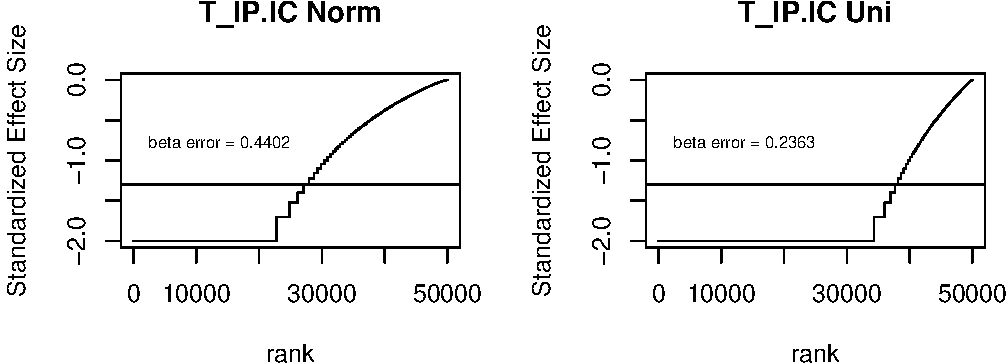
\includegraphics[width=\maxwidth]{figure/Internal_filter_results_pval_local-1} 

}

\caption[Beta-error mixing all strength of internal filtering]{Beta-error mixing all strength of internal filtering: Standardized effect size of $T_{IP/IC}$ are ordered and plot. The black line represent the value of 0.05. Consequently, p-values above this line are false-negative cases. Norm: normal distribution, Uni: uniforme distribution. \label{fig:Internal_filter_results_pval_local}}
\end{figure}


\end{knitrout}

The beta-error is very high and thus the power of $T_{IP/IC}$ can \textit{prima facie} seen as problematic (Fig. \ref{fig:Internal_filter_results_pval_local}). But here we mingle the p-value for several parameters values. Thus it is far more informative to see the power of the test in relation to the initial parameters values. We represent standardized effect sizes values (hereafter called SES) in relation to the strength of internal filter to determine the parameters values which allow a satisfactory power of $T_{IP/IC}$.

As we add stochasticity around the initial parameters values, we can measure the strength of internal filtering by (i) the initial parameter values or (ii) by calculating the modeled parameter values\footnote{\textit{i.e.} the parameter values after adding stochasticity}.
 
  \subsubsubsection {Local $T_{IP/IC}$ SES values against initial parameter values}

\begin{knitrout}\small
\definecolor{shadecolor}{rgb}{0.969, 0.969, 0.969}\color{fgcolor}\begin{kframe}
\begin{alltt}
\hlstd{meanSES.2loc.norm_Tipic} \hlkwb{<-} \hlkwd{unlist}\hlstd{(}\hlkwd{lapply}\hlstd{(res.simu2,} \hlkwa{function}\hlstd{(}\hlkwc{x}\hlstd{)}
             \hlkwd{ses.listofindex}\hlstd{(}\hlkwd{as.listofindex}\hlstd{(x))}
             \hlopt{$}\hlstd{index_1_1}\hlopt{$}\hlstd{ses[,} \hlnum{1}\hlstd{]))}

\hlstd{meanSES.2loc.uni_Tipic} \hlkwb{<-} \hlkwd{unlist}\hlstd{(}\hlkwd{lapply}\hlstd{(res.simu2,} \hlkwa{function}\hlstd{(}\hlkwc{x}\hlstd{)}
             \hlkwd{ses.listofindex}\hlstd{(}\hlkwd{as.listofindex}\hlstd{(x))}
             \hlopt{$}\hlstd{index_1_1}\hlopt{$}\hlstd{ses[,} \hlnum{2}\hlstd{]))}

\hlstd{SES.inf.MEAN.norm_Tipic} \hlkwb{<-} \hlkwd{unlist}\hlstd{(}\hlkwd{lapply}\hlstd{(res.simu2,} \hlkwa{function}\hlstd{(}\hlkwc{x}\hlstd{)}
             \hlkwd{ses.listofindex}\hlstd{(}\hlkwd{as.listofindex}\hlstd{(x))}
             \hlopt{$}\hlstd{index_1_1}\hlopt{$}\hlstd{ses.inf[,} \hlnum{1}\hlstd{]))}

\hlstd{SES.inf.MEAN.uni_Tipic} \hlkwb{<-} \hlkwd{unlist}\hlstd{(}\hlkwd{lapply}\hlstd{(res.simu2,} \hlkwa{function}\hlstd{(}\hlkwc{x}\hlstd{)}
             \hlkwd{ses.listofindex}\hlstd{(}\hlkwd{as.listofindex}\hlstd{(x))}
             \hlopt{$}\hlstd{index_1_1}\hlopt{$}\hlstd{ses.inf[,} \hlnum{2}\hlstd{]))}
\end{alltt}
\end{kframe}
\end{knitrout}

Now, we can plot SES of $T_{IP/IC}$ (Fig. \ref{fig:In_filter_results_plot_initparam}). The trait "a" normally distributed is in black and the uniform traits "b" is in purple. The colored rectangles represent the null model area with alpha = 5\%. Thus, when a point is outside these area, the modeled parameters are strong enough to detect the internal filter with a high power (beta-error $ < 0.05$).

  
\begin{knitrout}\small
\definecolor{shadecolor}{rgb}{0.969, 0.969, 0.969}\color{fgcolor}\begin{kframe}
\begin{alltt}
\hlstd{init_param} \hlkwb{<-} \hlstd{param_DIST_between_MEAN} \hlopt{/} \hlstd{sd_mean.param}
\hlstd{init_param.loc} \hlkwb{<-} \hlkwd{rep}\hlstd{(init_param,} \hlkwc{each} \hlstd{= Ncom)}

\hlkwd{plot}\hlstd{(meanSES.2loc.norm_Tipic, init_param.loc,} \hlkwc{pch} \hlstd{=} \hlnum{16}\hlstd{,} \hlkwc{col} \hlstd{=} \hlkwd{rgb}\hlstd{(}\hlnum{0}\hlstd{,} \hlnum{0}\hlstd{,} \hlnum{0}\hlstd{,} \hlnum{0.6}\hlstd{),}
     \hlkwc{xlim} \hlstd{=} \hlkwd{c}\hlstd{(}\hlkwd{min}\hlstd{(}\hlkwd{c}\hlstd{(}\hlkwd{unlist}\hlstd{(meanSES.2loc.norm_Tipic),} \hlkwd{unlist}\hlstd{(meanSES.2loc.uni_Tipic)),}
     \hlkwc{na.rm} \hlstd{= T),} \hlnum{0}\hlstd{),}
     \hlkwc{main} \hlstd{=} \hlstr{"Local T_IP.IC"}\hlstd{,}
     \hlkwc{xlab} \hlstd{=} \hlstr{"standardized effect size of T_IP.IC"}\hlstd{,}
     \hlkwc{ylab} \hlstd{=} \hlstr{"initial parameters: range/sd"}\hlstd{)}
\hlkwd{abline}\hlstd{(}\hlkwc{v} \hlstd{=} \hlkwd{mean}\hlstd{(SES.inf.MEAN.norm_Tipic,} \hlkwc{na.rm} \hlstd{= T))}

\hlkwd{points}\hlstd{(meanSES.2loc.uni_Tipic, init_param.loc,} \hlkwc{pch} \hlstd{=} \hlnum{16}\hlstd{,} \hlkwc{col} \hlstd{=} \hlkwd{rgb}\hlstd{(}\hlnum{0.5}\hlstd{,} \hlnum{0}\hlstd{,} \hlnum{1}\hlstd{,} \hlnum{0.6}\hlstd{))}
\hlkwd{abline}\hlstd{(}\hlkwc{v} \hlstd{=} \hlkwd{mean}\hlstd{(SES.inf.MEAN.uni_Tipic,} \hlkwc{na.rm} \hlstd{= T),} \hlkwc{col} \hlstd{=} \hlstr{"purple"}\hlstd{)}
\hlkwd{rect}\hlstd{(}\hlkwd{mean}\hlstd{(SES.inf.MEAN.norm_Tipic,} \hlkwc{na.rm} \hlstd{= T),} \hlopt{-}\hlnum{1}\hlstd{,} \hlnum{0}\hlstd{,} \hlkwd{max}\hlstd{(init_param)} \hlopt{+} \hlnum{1}\hlstd{,}
     \hlkwc{col} \hlstd{=} \hlkwd{rgb}\hlstd{(}\hlnum{0}\hlstd{,} \hlnum{0}\hlstd{,} \hlnum{0}\hlstd{,} \hlnum{0.3}\hlstd{),} \hlkwc{border} \hlstd{=} \hlnum{NA}\hlstd{)}
\hlkwd{rect}\hlstd{(}\hlkwd{mean}\hlstd{(SES.inf.MEAN.uni_Tipic,} \hlkwc{na.rm} \hlstd{= T),} \hlnum{0}\hlstd{,} \hlnum{0}\hlstd{,} \hlkwd{max}\hlstd{(init_param),}
     \hlkwc{col} \hlstd{=} \hlkwd{rgb}\hlstd{(}\hlnum{0.5}\hlstd{,} \hlnum{0}\hlstd{,} \hlnum{1}\hlstd{,} \hlnum{0.3}\hlstd{),} \hlkwc{border} \hlstd{=} \hlnum{NA}\hlstd{)}
\end{alltt}
\end{kframe}\begin{figure}

{\centering 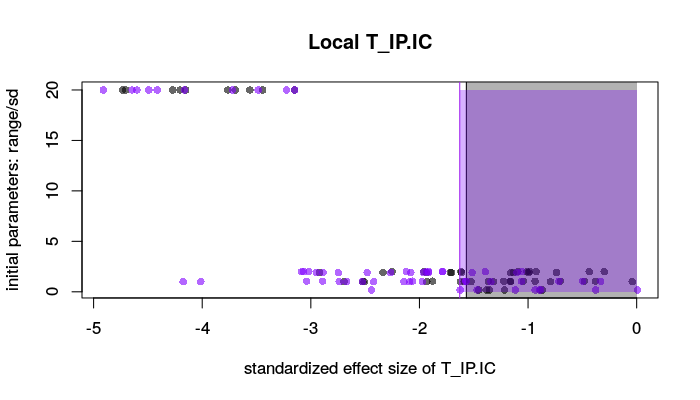
\includegraphics[width=\maxwidth]{figure/In_filter_results_plot_initparam-1} 

}

\caption[Local $T_{IP/IC}$ SES and initial parameters values]{Local $T_{IP/IC}$ SES and initial parameters values: Standardized effect size of $T_{IP/IC}$ in function of the strength of internal filter defined by the ratio of the initial range parameter by the initial standard error parameter. Colored area represent the mean confidence interval of SES values ($alpha = 0.95$). Trait a (normal) in black and b (uniform) in purple.\label{fig:In_filter_results_plot_initparam}}
\end{figure}


\end{knitrout}
 
  
For each initial parameters values we can calculate the proportion of case where we do not reject the null hypothesis while this hypothesis is wrong (\textit{i.e.} the Beta-error). The next chunk only show the calculation for the $T_{IC/IR}$ metrics on the trait "a".

\begin{knitrout}\small
\definecolor{shadecolor}{rgb}{0.969, 0.969, 0.969}\color{fgcolor}\begin{kframe}
\begin{alltt}
\hlstd{beta_sd_norm_Tipic} \hlkwb{<-}
 \hlstd{(}\hlkwd{unlist}\hlstd{(}\hlkwd{lapply}\hlstd{(}\hlkwd{by}\hlstd{(}\hlkwd{cbind}\hlstd{(meanSES.2loc.norm_Tipic, SES.inf.MEAN.norm_Tipic),}
     \hlkwd{rep}\hlstd{(sd_mean.param,} \hlkwc{each} \hlstd{= Ncom),} \hlkwa{function}\hlstd{(}\hlkwc{x}\hlstd{) x[,}\hlnum{1}\hlstd{]} \hlopt{>} \hlstd{x[,}\hlnum{2}\hlstd{]),}
     \hlkwa{function}\hlstd{(}\hlkwc{x}\hlstd{)} \hlkwd{sum}\hlstd{(x,} \hlkwc{na.rm} \hlstd{= T)))}\hlopt{+}\hlnum{1}\hlstd{)}\hlopt{/}\hlstd{(}\hlnum{10} \hlopt{*} \hlstd{N_repet_Param} \hlopt{+} \hlnum{1}\hlstd{)}
\hlstd{beta_range_norm_Tipic} \hlkwb{<-}
 \hlstd{(}\hlkwd{unlist}\hlstd{(}\hlkwd{lapply}\hlstd{(}\hlkwd{by}\hlstd{(}\hlkwd{cbind}\hlstd{(meanSES.2loc.norm_Tipic, SES.inf.MEAN.norm_Tipic),}
     \hlkwd{rep}\hlstd{(param_DIST_between_MEAN,} \hlkwc{each} \hlstd{= Ncom),} \hlkwa{function}\hlstd{(}\hlkwc{x}\hlstd{) x[,}\hlnum{1}\hlstd{]} \hlopt{>} \hlstd{x[,}\hlnum{2}\hlstd{]),}
     \hlkwa{function}\hlstd{(}\hlkwc{x}\hlstd{)} \hlkwd{sum}\hlstd{(x,} \hlkwc{na.rm} \hlstd{= T)))}\hlopt{+}\hlnum{1}\hlstd{)}\hlopt{/}\hlstd{(}\hlnum{10} \hlopt{*} \hlstd{N_repet_Param} \hlopt{+} \hlnum{1}\hlstd{)}

\hlstd{beta_sd_uni_Tipic} \hlkwb{<-}
 \hlstd{(}\hlkwd{unlist}\hlstd{(}\hlkwd{lapply}\hlstd{(}\hlkwd{by}\hlstd{(}\hlkwd{cbind}\hlstd{(meanSES.2loc.uni_Tipic, SES.inf.MEAN.uni_Tipic),}
     \hlkwd{rep}\hlstd{(sd_mean.param,} \hlkwc{each} \hlstd{= Ncom),} \hlkwa{function}\hlstd{(}\hlkwc{x}\hlstd{) x[,}\hlnum{1}\hlstd{]} \hlopt{>} \hlstd{x[,}\hlnum{2}\hlstd{]),}
     \hlkwa{function}\hlstd{(}\hlkwc{x}\hlstd{)} \hlkwd{sum}\hlstd{(x,} \hlkwc{na.rm} \hlstd{= T)))}\hlopt{+}\hlnum{1}\hlstd{)}\hlopt{/}\hlstd{(}\hlnum{10} \hlopt{*} \hlstd{N_repet_Param} \hlopt{+} \hlnum{1}\hlstd{)}
\hlstd{beta_range_uni_Tipic} \hlkwb{<-}
 \hlstd{(}\hlkwd{unlist}\hlstd{(}\hlkwd{lapply}\hlstd{(}\hlkwd{by}\hlstd{(}\hlkwd{cbind}\hlstd{(meanSES.2loc.uni_Tipic, SES.inf.MEAN.uni_Tipic),}
     \hlkwd{rep}\hlstd{(param_DIST_between_MEAN,} \hlkwc{each} \hlstd{= Ncom),} \hlkwa{function}\hlstd{(}\hlkwc{x}\hlstd{) x[,}\hlnum{1}\hlstd{]} \hlopt{>} \hlstd{x[,}\hlnum{2}\hlstd{]),}
     \hlkwa{function}\hlstd{(}\hlkwc{x}\hlstd{)} \hlkwd{sum}\hlstd{(x,} \hlkwc{na.rm} \hlstd{= T)))}\hlopt{+}\hlnum{1}\hlstd{)}\hlopt{/}\hlstd{(}\hlnum{10} \hlopt{*} \hlstd{N_repet_Param} \hlopt{+} \hlnum{1}\hlstd{)}

\hlstd{res_beta_Tipic} \hlkwb{<-} \hlkwd{rbind}\hlstd{(}\hlkwd{rev}\hlstd{(beta_sd_norm_Tipic),} \hlkwd{rev}\hlstd{(beta_sd_uni_Tipic),}
      \hlstd{beta_range_norm_Tipic, beta_range_uni_Tipic)}
\hlkwd{colnames}\hlstd{(res_beta_Tipic)} \hlkwb{<-} \hlkwd{paste}\hlstd{(}\hlstr{"str"}\hlstd{,} \hlnum{1}\hlopt{:}\hlkwd{ncol}\hlstd{(res_beta_Tipic))}
\hlkwd{rownames}\hlstd{(res_beta_Tipic)} \hlkwb{<-} \hlkwd{c}\hlstd{(}\hlstr{"effect of sd (a)"}\hlstd{,} \hlstr{"effect of sd (b)"}\hlstd{,}
        \hlstr{"effect of range (a)"}\hlstd{,} \hlstr{"effect of range (b)"}\hlstd{)}
\end{alltt}
\end{kframe}
\end{knitrout}

\begin{kframe}
\begin{alltt}
\hlkwd{print}\hlstd{(}\hlkwd{xtable}\hlstd{(res_beta_Tipic,} \hlkwc{caption} \hlstd{=} \hlstr{'Local beta-error of $T_\{IP/IC\}$ in function 
             of the strength of internal filtering. str: strength. Trait a is 
             normally distributed and trait b is uniformally distributed.'}\hlstd{,}
             \hlkwc{label} \hlstd{=} \hlstr{"tab:local_beta_error_xtable"}\hlstd{),}
      \hlkwc{caption.placement} \hlstd{=} \hlstr{"top"}\hlstd{,} \hlkwc{size} \hlstd{=} \hlstr{"small"}\hlstd{)}
\end{alltt}
\end{kframe}% latex table generated in R 3.1.2 by xtable 1.7-4 package
% Tue Jan 13 20:18:01 2015
\begin{table}[ht]
\centering
\caption{Local beta-error of $T_{IP/IC}$ in function 
             of the strength of internal filtering. str: strength. Trait a is 
             normally distributed and trait b is uniformally distributed.} 
\label{tab:local_beta_error_xtable}
{\small
\begin{tabular}{rrrrrrrrrrr}
  \hline
 & str 1 & str 2 & str 3 & str 4 & str 5 & str 6 & str 7 & str 8 & str 9 & str 10 \\ 
  \hline
effect of sd (a) & 0.67 & 0.66 & 0.60 & 0.60 & 0.41 & 0.35 & 0.30 & 0.20 & 0.11 & 0.07 \\ 
  effect of sd (b) & 0.37 & 0.38 & 0.34 & 0.33 & 0.18 & 0.15 & 0.13 & 0.06 & 0.02 & 0.01 \\ 
  effect of range (a) & 0.82 & 0.73 & 0.65 & 0.51 & 0.37 & 0.32 & 0.22 & 0.14 & 0.11 & 0.09 \\ 
  effect of range (b) & 0.66 & 0.51 & 0.39 & 0.24 & 0.10 & 0.05 & 0.02 & 0.01 & 0.00 & 0.00 \\ 
   \hline
\end{tabular}
}
\end{table}

 

Now we can see the beta-error for each strength in table \ref{tab:local_beta_error_xtable}. A high value of range and a low value of standard error defined a high strength of filtering. For example, in the case of a trait normally distributed, the proportion of false negative is 66.87\% for the higher value of standard errors and thus for the lower strength of internal filtering. The good behavior of the function \texttt{Tstats} is ascertain by the decrease of beta-error along increasing strength of filter.
 
 
  \subsubsubsection {Local $T_{IP/IC}$ SES values against modeled parameter values}
  
  First we need to calculate the modeled parameter values. Here again we calculate the strength of internal filtering by dividing the range of values in communities by their standard error.
  
\begin{knitrout}\small
\definecolor{shadecolor}{rgb}{0.969, 0.969, 0.969}\color{fgcolor}\begin{kframe}
\begin{alltt}
\hlstd{mean_dist_sp.interm} \hlkwb{<-} \hlkwd{t}\hlstd{(}\hlkwd{matrix}\hlstd{(}\hlkwd{unlist}\hlstd{(}\hlkwd{lapply}\hlstd{(mean_dist_sp,} \hlkwa{function}\hlstd{(}\hlkwc{x}\hlstd{) x)),} \hlkwc{nrow} \hlstd{=} \hlnum{2}\hlstd{))}
\hlstd{mean_sd_of_com} \hlkwb{<-} \hlkwd{unlist}\hlstd{(}\hlkwd{lapply}\hlstd{(sd.sp_stock2,} \hlkwa{function}\hlstd{(}\hlkwc{x}\hlstd{)} \hlkwd{mean}\hlstd{(x)))}

\hlstd{modeled_param_norm} \hlkwb{<-} \hlstd{mean_dist_sp.interm[,} \hlnum{1}\hlstd{]} \hlopt{/} \hlstd{mean_sd_of_com}
\hlstd{modeled_param_uni} \hlkwb{<-} \hlstd{mean_dist_sp.interm[,} \hlnum{2}\hlstd{]} \hlopt{/} \hlstd{mean_sd_of_com}
\hlstd{modeled_param_norm.loc} \hlkwb{<-} \hlkwd{rep}\hlstd{(modeled_param_norm,} \hlkwc{each} \hlstd{= Ncom)}
\hlstd{modeled_param_uni.loc} \hlkwb{<-} \hlkwd{rep}\hlstd{(modeled_param_uni,} \hlkwc{each} \hlstd{= Ncom)}
\end{alltt}
\end{kframe}
\end{knitrout}

\begin{knitrout}\small
\definecolor{shadecolor}{rgb}{0.969, 0.969, 0.969}\color{fgcolor}\begin{kframe}
\begin{alltt}
\hlkwd{plot}\hlstd{(meanSES.2loc.norm_Tipic, modeled_param_norm.loc,} \hlkwc{pch} \hlstd{=} \hlnum{16}\hlstd{,} \hlkwc{col} \hlstd{=} \hlkwd{rgb}\hlstd{(}\hlnum{0}\hlstd{,} \hlnum{0}\hlstd{,} \hlnum{0}\hlstd{,} \hlnum{0.6}\hlstd{),}
     \hlkwc{xlim} \hlstd{=} \hlkwd{c}\hlstd{(}\hlkwd{min}\hlstd{(}\hlkwd{c}\hlstd{(}\hlkwd{unlist}\hlstd{(meanSES.2loc.norm_Tipic),} \hlkwd{unlist}\hlstd{(meanSES.2loc.uni_Tipic)),}
              \hlkwc{na.rm} \hlstd{= T),} \hlnum{0}\hlstd{),}
     \hlkwc{ylim} \hlstd{=} \hlkwd{c}\hlstd{(}\hlkwd{min}\hlstd{(}\hlkwd{c}\hlstd{(modeled_param_norm.loc, modeled_param_uni.loc),} \hlkwc{na.rm} \hlstd{= T),}
              \hlkwd{max}\hlstd{(}\hlkwd{c}\hlstd{(modeled_param_norm.loc, modeled_param_uni.loc),} \hlkwc{na.rm} \hlstd{= T)),}
     \hlkwc{main} \hlstd{=} \hlstr{"Local T_IP.IC"}\hlstd{,}
     \hlkwc{xlab} \hlstd{=} \hlstr{"standardized effect size of T_IP.IC"}\hlstd{,}
     \hlkwc{ylab} \hlstd{=} \hlstr{"modeled parameters: range/sd"}\hlstd{)}
\hlkwd{abline}\hlstd{(}\hlkwc{v} \hlstd{=} \hlkwd{mean}\hlstd{(SES.inf.MEAN.norm_Tipic,} \hlkwc{na.rm} \hlstd{= T))}

\hlkwd{points}\hlstd{(meanSES.2loc.uni_Tipic, modeled_param_uni.loc,} \hlkwc{pch} \hlstd{=} \hlnum{16}\hlstd{,} \hlkwc{col} \hlstd{=} \hlkwd{rgb}\hlstd{(}\hlnum{0.5}\hlstd{,} \hlnum{0}\hlstd{,} \hlnum{1}\hlstd{,} \hlnum{0.6}\hlstd{))}
\hlkwd{abline}\hlstd{(}\hlkwc{v} \hlstd{=} \hlkwd{mean}\hlstd{(SES.inf.MEAN.uni_Tipic,} \hlkwc{na.rm} \hlstd{= T),} \hlkwc{col} \hlstd{=} \hlstr{"purple"}\hlstd{)}
\hlkwd{rect}\hlstd{(}\hlkwd{mean}\hlstd{(SES.inf.MEAN.norm_Tipic,} \hlkwc{na.rm} \hlstd{= T),} \hlopt{-}\hlnum{1}\hlstd{,} \hlnum{0}\hlstd{,} \hlkwd{max}\hlstd{(modeled_param_norm.loc)} \hlopt{+} \hlnum{1}\hlstd{,}
     \hlkwc{col} \hlstd{=} \hlkwd{rgb}\hlstd{(}\hlnum{0}\hlstd{,} \hlnum{0}\hlstd{,} \hlnum{0}\hlstd{,} \hlnum{0.3}\hlstd{),} \hlkwc{border} \hlstd{=} \hlnum{NA}\hlstd{)}
\hlkwd{rect}\hlstd{(}\hlkwd{mean}\hlstd{(SES.inf.MEAN.uni_Tipic,} \hlkwc{na.rm} \hlstd{= T),} \hlnum{0}\hlstd{,} \hlnum{0}\hlstd{,} \hlkwd{max}\hlstd{(modeled_param_uni.loc),}
     \hlkwc{col} \hlstd{=} \hlkwd{rgb}\hlstd{(}\hlnum{0.5}\hlstd{,} \hlnum{0}\hlstd{,} \hlnum{1}\hlstd{,} \hlnum{0.3}\hlstd{),} \hlkwc{border} \hlstd{=} \hlnum{NA}\hlstd{)}
\end{alltt}
\end{kframe}\begin{figure}

{\centering 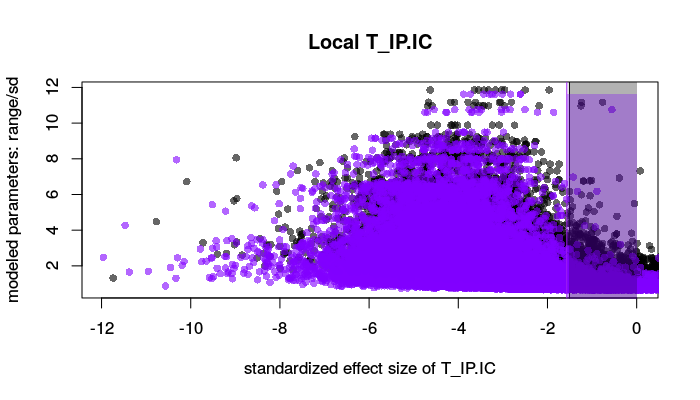
\includegraphics[width=\maxwidth]{figure/In_filter_results_plot_modeledparam-1} 

}

\caption[Local $T_{IP/IC}$ SES and modeled parameters values]{Local $T_{IP/IC}$ SES and modeled parameters values: Standardized effect size of $T_{IP/IC}$ in function of the strength of internal filter defined by the ratio of the modeled range parameter by the modeled standard error parameter. The colored rectangles represent the mean confidence interval for SES values ($alpha = 0.95$). Trait a (normal) in black and b (uniform) in purple.\label{fig:In_filter_results_plot_modeledparam}}
\end{figure}


\end{knitrout}

There is a very hich correlation coefficient between initial and modeled parameter either for the range (trait a: Pearson correlation = 0.325; trait b: Pearson correlation = 0.36) and for the standard error(trait a and b: Pearson correlation = 0.997). Consequently the consistency between the figures \ref{fig:In_filter_results_plot_initparam} and  \ref{fig:In_filter_results_plot_modeledparam} is not suprising. 
 
 \subsubsection {Global p-values results for $T_{IP/IC}$}
In contrast with local p-values, we call global p-values the p-values corresponding to one indice for one trait across all the communities. 

  \subsubsubsection {Global $T_{IP/IC}$ SES values against initial parameter values}
  
Again, this first results mix different initial parameter values. Now, we can plot the SES values in relation to the strength of the internal filter assessed by the two parameters (either the initial values: \texttt{mean\_range\_between\_com} and \texttt{mean\_sd\_of\_com} or the modeled values \texttt{mean\_{}range\_{}com} and \texttt{sd.com\_{}stock2} \footnote{This modeled values are stochastic versions of the initial values.}). 

First, we need to compute the SES values from simulations.
\begin{knitrout}\small
\definecolor{shadecolor}{rgb}{0.969, 0.969, 0.969}\color{fgcolor}\begin{kframe}
\begin{alltt}
\hlstd{meanSES.2glob.norm_Tipic} \hlkwb{<-} \hlkwd{unlist}\hlstd{(}\hlkwd{lapply}\hlstd{(res.simu2,} \hlkwa{function}\hlstd{(}\hlkwc{x}\hlstd{)}
           \hlkwd{mean}\hlstd{(}\hlkwd{ses.listofindex}\hlstd{(}\hlkwd{as.listofindex}\hlstd{(x))}
             \hlopt{$}\hlstd{index_1_1}\hlopt{$}\hlstd{ses[,}\hlnum{1}\hlstd{],} \hlkwc{na.rm} \hlstd{= T)))}
\hlstd{meanSES.2glob.uni_Tipic} \hlkwb{<-} \hlkwd{unlist}\hlstd{(}\hlkwd{lapply}\hlstd{(res.simu2,} \hlkwa{function}\hlstd{(}\hlkwc{x}\hlstd{)}
           \hlkwd{mean}\hlstd{(}\hlkwd{ses.listofindex}\hlstd{(}\hlkwd{as.listofindex}\hlstd{(x))}
             \hlopt{$}\hlstd{index_1_1}\hlopt{$}\hlstd{ses[,}\hlnum{2}\hlstd{],} \hlkwc{na.rm} \hlstd{= T)))}

\hlstd{meanSES.INF_glob.norm_Tipic} \hlkwb{<-} \hlkwd{unlist}\hlstd{(}\hlkwd{lapply}\hlstd{(res.simu2,} \hlkwa{function}\hlstd{(}\hlkwc{x}\hlstd{)}
           \hlkwd{mean}\hlstd{(}\hlkwd{ses.listofindex}\hlstd{(}\hlkwd{as.listofindex}\hlstd{(x))}
             \hlopt{$}\hlstd{index_1_1}\hlopt{$}\hlstd{ses.inf[,} \hlnum{1}\hlstd{],} \hlkwc{na.rm} \hlstd{= T)))}
\hlstd{meanSES.INF_glob.uni_Tipic} \hlkwb{<-} \hlkwd{unlist}\hlstd{(}\hlkwd{lapply}\hlstd{(res.simu2,} \hlkwa{function}\hlstd{(}\hlkwc{x}\hlstd{)}
           \hlkwd{mean}\hlstd{(}\hlkwd{ses.listofindex}\hlstd{(}\hlkwd{as.listofindex}\hlstd{(x))}
             \hlopt{$}\hlstd{index_1_1}\hlopt{$}\hlstd{ses.inf[,} \hlnum{2}\hlstd{],} \hlkwc{na.rm} \hlstd{= T)))}
\end{alltt}
\end{kframe}
\end{knitrout}

Plot the result against initial parameters (Fig. \ref{fig:Internal_filter_Results_plots_initial_param}).


\begin{knitrout}\small
\definecolor{shadecolor}{rgb}{0.969, 0.969, 0.969}\color{fgcolor}\begin{kframe}
\begin{alltt}
\hlkwd{plot}\hlstd{(meanSES.2glob.norm_Tipic, init_param,} \hlkwc{pch} \hlstd{=} \hlnum{16}\hlstd{,} \hlkwc{col} \hlstd{=} \hlkwd{rgb}\hlstd{(}\hlnum{0}\hlstd{,} \hlnum{0}\hlstd{,} \hlnum{0}\hlstd{,} \hlnum{0.6}\hlstd{),}
     \hlkwc{main} \hlstd{=} \hlstr{"Global T_IP.IC"}\hlstd{,}
     \hlkwc{xlim} \hlstd{=} \hlkwd{c}\hlstd{(}\hlkwd{min}\hlstd{(}\hlkwd{c}\hlstd{(meanSES.2glob.norm_Tipic, meanSES.2glob.uni_Tipic),}
            \hlkwc{na.rm} \hlstd{= T),} \hlnum{0}\hlstd{),}
     \hlkwc{xlab} \hlstd{=} \hlstr{"standardized effect size of T_IP.IC"}\hlstd{,}
     \hlkwc{ylab} \hlstd{=} \hlstr{"initial parameters: range/sd"}\hlstd{)}
\hlkwd{points}\hlstd{(meanSES.2glob.uni_Tipic, init_param,} \hlkwc{pch} \hlstd{=} \hlnum{16}\hlstd{,} \hlkwc{col} \hlstd{=} \hlkwd{rgb}\hlstd{(}\hlnum{0.5}\hlstd{,} \hlnum{0}\hlstd{,} \hlnum{1}\hlstd{,} \hlnum{0.6}\hlstd{),)}
\hlkwd{abline}\hlstd{(}\hlkwc{v} \hlstd{=} \hlkwd{mean}\hlstd{(meanSES.INF_glob.norm_Tipic,} \hlkwc{na.rm} \hlstd{= T))}
\hlkwd{abline}\hlstd{(}\hlkwc{v} \hlstd{=} \hlkwd{mean}\hlstd{(meanSES.INF_glob.uni_Tipic,} \hlkwc{na.rm} \hlstd{= T),} \hlkwc{col} \hlstd{=} \hlstr{"purple"}\hlstd{)}
\hlkwd{rect}\hlstd{(}\hlkwd{mean}\hlstd{(meanSES.INF_glob.norm_Tipic,} \hlkwc{na.rm} \hlstd{= T),} \hlopt{-}\hlnum{1}\hlstd{,} \hlnum{0}\hlstd{,} \hlkwd{max}\hlstd{(modeled_param_norm.loc)} \hlopt{+} \hlnum{1}\hlstd{,}
     \hlkwc{col} \hlstd{=} \hlkwd{rgb}\hlstd{(}\hlnum{0}\hlstd{,} \hlnum{0}\hlstd{,} \hlnum{0}\hlstd{,} \hlnum{0.3}\hlstd{),} \hlkwc{border} \hlstd{=} \hlnum{NA}\hlstd{)}
\hlkwd{rect}\hlstd{(}\hlkwd{mean}\hlstd{(meanSES.INF_glob.uni_Tipic,} \hlkwc{na.rm} \hlstd{= T),} \hlnum{0}\hlstd{,} \hlnum{0}\hlstd{,} \hlkwd{max}\hlstd{(modeled_param_uni.loc),}
     \hlkwc{col} \hlstd{=} \hlkwd{rgb}\hlstd{(}\hlnum{0.5}\hlstd{,} \hlnum{0}\hlstd{,} \hlnum{1}\hlstd{,} \hlnum{0.3}\hlstd{),} \hlkwc{border} \hlstd{=} \hlnum{NA}\hlstd{)}
\end{alltt}
\end{kframe}\begin{figure}

{\centering 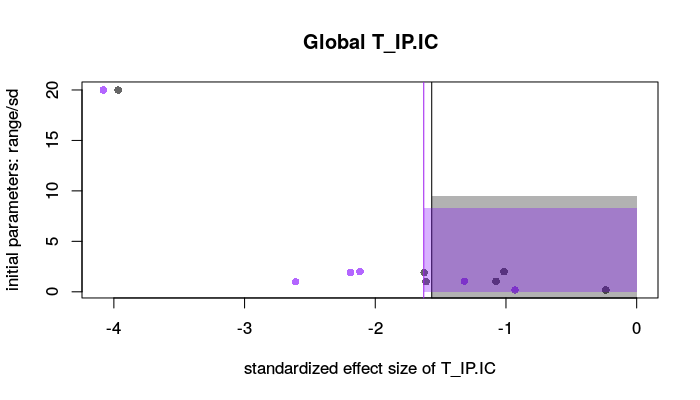
\includegraphics[width=\maxwidth]{figure/Internal_filter_Results_plots_initial_param-1} 

}

\caption[Global $T_{IP/IC}$ SES and initial parameters values]{Global $T_{IP/IC}$ SES and initial parameters values: Standardized effect size of $T_{IP/IC}$ in function of the strength of internal filter defined by the ratio of the inital range parameter by the initial standard error parameter. Colored area represent the mean confidence interval of SES values ($alpha = 0.95$). Trait a (normal) in black and b (uniform) in purple.\label{fig:Internal_filter_Results_plots_initial_param}}
\end{figure}


\end{knitrout}



  \subsubsubsection {Global $T_{IP/IC}$ SES values against modeled parameter values}
  
We can verify the consistency of our results by plotting SES values against the modeled parameters values (Fig. \ref{fig:Internal_filter_Results_plots_modeled_param} and \ref{fig:Internal_filter_Results_plots_modeled_param2}). 

\begin{knitrout}\small
\definecolor{shadecolor}{rgb}{0.969, 0.969, 0.969}\color{fgcolor}\begin{kframe}
\begin{alltt}
\hlstd{mean_dist_sp.interm} \hlkwb{<-} \hlkwd{t}\hlstd{(}\hlkwd{matrix}\hlstd{(}\hlkwd{unlist}\hlstd{(}\hlkwd{lapply}\hlstd{(mean_dist_sp,} \hlkwa{function}\hlstd{(}\hlkwc{x}\hlstd{) x)),} \hlkwc{nrow} \hlstd{=} \hlnum{2}\hlstd{))}
\hlstd{mean_sd_of_com} \hlkwb{<-} \hlkwd{unlist}\hlstd{(}\hlkwd{lapply}\hlstd{(sd.sp_stock2,} \hlkwa{function}\hlstd{(}\hlkwc{x}\hlstd{)} \hlkwd{mean}\hlstd{(x)))}

\hlstd{modeled_param_norm} \hlkwb{<-} \hlstd{mean_dist_sp.interm[,} \hlnum{1}\hlstd{]} \hlopt{/} \hlstd{mean_sd_of_com}
\hlstd{modeled_param_uni} \hlkwb{<-} \hlstd{mean_dist_sp.interm[,} \hlnum{2}\hlstd{]} \hlopt{/} \hlstd{mean_sd_of_com}

\hlkwd{plot}\hlstd{(meanSES.2glob.norm_Tipic, modeled_param_norm,} \hlkwc{pch} \hlstd{=} \hlnum{16}\hlstd{,}
     \hlkwc{main} \hlstd{=} \hlstr{"Global T_IP.IC"}\hlstd{,}
     \hlkwc{xlim} \hlstd{=} \hlkwd{c}\hlstd{(}\hlkwd{min}\hlstd{(}\hlkwd{c}\hlstd{(meanSES.2glob.norm_Tipic, meanSES.2glob.uni_Tipic),}
              \hlkwc{na.rm} \hlstd{= T),} \hlnum{0}\hlstd{),}
     \hlkwc{ylim} \hlstd{=} \hlkwd{c}\hlstd{(}\hlkwd{min}\hlstd{(}\hlkwd{c}\hlstd{(modeled_param_norm, modeled_param_uni),} \hlkwc{na.rm} \hlstd{= T),}
     \hlkwd{max}\hlstd{(}\hlkwd{c}\hlstd{(modeled_param_norm, modeled_param_uni),} \hlkwc{na.rm} \hlstd{= T)),}
     \hlkwc{xlab} \hlstd{=} \hlstr{"standardized effect size of T_IP.IC"}\hlstd{,}
     \hlkwc{ylab} \hlstd{=} \hlstr{"modeled parameters: range/sd"}\hlstd{)}
\hlkwd{points}\hlstd{(meanSES.2glob.uni_Tipic, modeled_param_uni,} \hlkwc{pch} \hlstd{=} \hlnum{16}\hlstd{,} \hlkwc{col} \hlstd{=} \hlkwd{rgb}\hlstd{(}\hlnum{0.5}\hlstd{,} \hlnum{0}\hlstd{,} \hlnum{1}\hlstd{,} \hlnum{0.6}\hlstd{))}
\hlkwd{abline}\hlstd{(}\hlkwc{v} \hlstd{=} \hlkwd{mean}\hlstd{(meanSES.INF_glob.norm_Tipic,} \hlkwc{na.rm} \hlstd{= T))}
\hlkwd{abline}\hlstd{(}\hlkwc{v} \hlstd{=} \hlkwd{mean}\hlstd{(meanSES.INF_glob.uni_Tipic,} \hlkwc{na.rm} \hlstd{= T),} \hlkwc{col} \hlstd{=} \hlstr{"purple"}\hlstd{)}
\hlkwd{rect}\hlstd{(}\hlkwd{mean}\hlstd{(meanSES.INF_glob.norm_Tipic,} \hlkwc{na.rm} \hlstd{= T),} \hlopt{-}\hlnum{1}\hlstd{,} \hlnum{0}\hlstd{,} \hlkwd{max}\hlstd{(modeled_param_norm)} \hlopt{+} \hlnum{1}\hlstd{,}
     \hlkwc{col} \hlstd{=} \hlkwd{rgb}\hlstd{(}\hlnum{0}\hlstd{,} \hlnum{0}\hlstd{,} \hlnum{0}\hlstd{,} \hlnum{0.3}\hlstd{),} \hlkwc{border} \hlstd{=} \hlnum{NA}\hlstd{)}
\hlkwd{rect}\hlstd{(}\hlkwd{mean}\hlstd{(meanSES.INF_glob.uni_Tipic,} \hlkwc{na.rm} \hlstd{= T),} \hlnum{0}\hlstd{,} \hlnum{0}\hlstd{,} \hlkwd{max}\hlstd{(modeled_param_uni),}
     \hlkwc{col} \hlstd{=} \hlkwd{rgb}\hlstd{(}\hlnum{0.5}\hlstd{,} \hlnum{0}\hlstd{,} \hlnum{1}\hlstd{,} \hlnum{0.3}\hlstd{),} \hlkwc{border} \hlstd{=} \hlnum{NA}\hlstd{)}
\end{alltt}
\end{kframe}\begin{figure}

{\centering 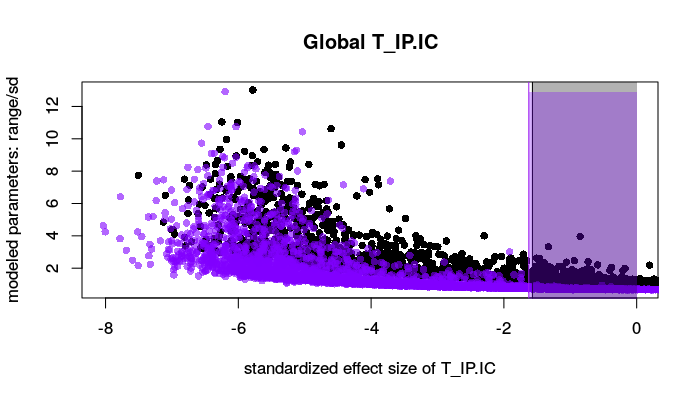
\includegraphics[width=\maxwidth]{figure/Internal_filter_Results_plots_modeled_param-1} 

}

\caption[Global $T_{IP/IC}$ SES and modeled parameters values]{Global $T_{IP/IC}$ SES and modeled parameters values: Standardized effect size of $T_{IP/IC}$ in function of the strength of internal filter defined by the ratio of the modeled range parameter by the modeled standard error parameter. Colored area represent the mean confidence interval of SES values ($alpha = 0.95$). Trait a (normal) in black and b (uniform) in purple.\label{fig:Internal_filter_Results_plots_modeled_param}}
\end{figure}


\end{knitrout}

  \subsection {Conclusion on the power of $T_{IP/IC}$ to detect internal filtering}

To conclude on the power of $T_{IP/IC}$ to detect internal filtering, we compute exponential linear model and identify the strength from which the beta-error is inferior to 0.05. This strength is define by the two ratio of the initial parameters \texttt{param\_DIST\_between\_MEAN} and \texttt{sd\_mean.param}. 

\begin{knitrout}\small
\definecolor{shadecolor}{rgb}{0.969, 0.969, 0.969}\color{fgcolor}\begin{kframe}
\begin{alltt}
\hlkwd{plot}\hlstd{(meanSES.2loc.norm_Tipic} \hlopt{~} \hlstd{init_param.loc,} \hlkwc{col} \hlstd{=} \hlkwd{rgb}\hlstd{(}\hlnum{0}\hlstd{,} \hlnum{0}\hlstd{,} \hlnum{0}\hlstd{,} \hlnum{0.2}\hlstd{),}
     \hlkwc{ylim} \hlstd{=} \hlkwd{c}\hlstd{(}\hlkwd{min}\hlstd{(}\hlkwd{c}\hlstd{(meanSES.2loc.norm_Tipic , meanSES.2loc.uni_Tipic,}
                  \hlstd{meanSES.2glob.norm_Tipic, meanSES.2glob.uni_Tipic),} \hlkwc{na.rm} \hlstd{= T),} \hlnum{0}\hlstd{),}
     \hlkwc{main} \hlstd{=} \hlstr{"T_IP.IC"}\hlstd{,}
     \hlkwc{ylab} \hlstd{=} \hlstr{"standardized effect size of T_IP.IC"}\hlstd{,}
     \hlkwc{xlab} \hlstd{=} \hlstr{"initial parameters: range/sd"}\hlstd{,}
     \hlkwc{type} \hlstd{=} \hlstr{"n"}\hlstd{)}
\hlcom{#points(meanSES.2loc.uni_Tipic ~ init_param.loc, col = rgb(0.5, 0, 1, 0.2))}

\hlkwd{points}\hlstd{(meanSES.2glob.norm_Tipic} \hlopt{~} \hlstd{init_param,} \hlkwc{pch} \hlstd{=} \hlnum{16}\hlstd{,} \hlkwc{col} \hlstd{=} \hlkwd{rgb}\hlstd{(}\hlnum{0}\hlstd{,} \hlnum{0}\hlstd{,} \hlnum{0}\hlstd{,} \hlnum{0.5}\hlstd{),}
       \hlkwc{cex} \hlstd{=} \hlnum{1.2}\hlstd{)}
\hlstd{lm.norm} \hlkwb{<-} \hlkwd{lm}\hlstd{(meanSES.2glob.norm_Tipic} \hlopt{~} \hlkwd{log}\hlstd{(init_param))}
\hlstd{lm.norm_conf} \hlkwb{<-} \hlkwd{confint}\hlstd{(lm.norm,} \hlkwc{level} \hlstd{=} \hlnum{0.90}\hlstd{)}
\hlkwd{curve}\hlstd{(lm.norm}\hlopt{$}\hlstd{coef[}\hlnum{1}\hlstd{]} \hlopt{+} \hlkwd{log}\hlstd{(x)} \hlopt{*} \hlstd{(lm.norm}\hlopt{$}\hlstd{coef[}\hlnum{2}\hlstd{]),} \hlkwc{add} \hlstd{= T,} \hlkwc{lwd} \hlstd{=} \hlnum{3}\hlstd{)}
\hlkwd{curve}\hlstd{(lm.norm_conf [}\hlnum{1}\hlstd{,} \hlnum{1}\hlstd{]} \hlopt{+} \hlkwd{log}\hlstd{(x)} \hlopt{*} \hlstd{lm.norm_conf [}\hlnum{2}\hlstd{,} \hlnum{1}\hlstd{],} \hlkwc{add} \hlstd{= T,} \hlkwc{lty} \hlstd{=} \hlnum{2}\hlstd{)}
\hlkwd{curve}\hlstd{(lm.norm_conf [}\hlnum{1}\hlstd{,} \hlnum{2}\hlstd{]} \hlopt{+} \hlkwd{log}\hlstd{(x)} \hlopt{*} \hlstd{lm.norm_conf [}\hlnum{2}\hlstd{,} \hlnum{2}\hlstd{],} \hlkwc{add} \hlstd{= T,} \hlkwc{lty} \hlstd{=} \hlnum{2}\hlstd{)}

\hlkwd{points}\hlstd{(meanSES.2glob.uni_Tipic} \hlopt{~} \hlstd{init_param,} \hlkwc{pch} \hlstd{=} \hlnum{16}\hlstd{,} \hlkwc{col} \hlstd{=} \hlkwd{rgb}\hlstd{(}\hlnum{0.5}\hlstd{,} \hlnum{0}\hlstd{,} \hlnum{1}\hlstd{,} \hlnum{0.5}\hlstd{),}
       \hlkwc{cex} \hlstd{=} \hlnum{1.2}\hlstd{)}
\hlstd{lm.uni} \hlkwb{<-} \hlkwd{lm}\hlstd{(meanSES.2glob.uni_Tipic} \hlopt{~} \hlkwd{log}\hlstd{(init_param))}
\hlstd{lm.uni_conf} \hlkwb{<-} \hlkwd{confint}\hlstd{(lm.uni,} \hlkwc{level} \hlstd{=} \hlnum{0.90}\hlstd{)}
\hlkwd{curve}\hlstd{(lm.uni}\hlopt{$}\hlstd{coef[}\hlnum{1}\hlstd{]} \hlopt{+} \hlkwd{log}\hlstd{(x)} \hlopt{*} \hlstd{(lm.uni}\hlopt{$}\hlstd{coef[}\hlnum{2}\hlstd{]),} \hlkwc{add} \hlstd{= T,} \hlkwc{lwd} \hlstd{=} \hlnum{3}\hlstd{,}
      \hlkwc{col} \hlstd{=} \hlkwd{rgb}\hlstd{(}\hlnum{0.5}\hlstd{,} \hlnum{0}\hlstd{,} \hlnum{1}\hlstd{,} \hlnum{1}\hlstd{))}
\hlkwd{curve}\hlstd{(lm.uni_conf [}\hlnum{1}\hlstd{,} \hlnum{1}\hlstd{]} \hlopt{+} \hlkwd{log}\hlstd{(x)} \hlopt{*} \hlstd{lm.uni_conf [}\hlnum{2}\hlstd{,} \hlnum{1}\hlstd{],} \hlkwc{add} \hlstd{= T,} \hlkwc{lty} \hlstd{=} \hlnum{2}\hlstd{,}
      \hlkwc{col} \hlstd{=} \hlkwd{rgb}\hlstd{(}\hlnum{0.5}\hlstd{,} \hlnum{0}\hlstd{,} \hlnum{1}\hlstd{,} \hlnum{1}\hlstd{))}
\hlkwd{curve}\hlstd{(lm.uni_conf [}\hlnum{1}\hlstd{,} \hlnum{2}\hlstd{]} \hlopt{+} \hlkwd{log}\hlstd{(x)} \hlopt{*} \hlstd{lm.uni_conf [}\hlnum{2}\hlstd{,} \hlnum{2}\hlstd{],} \hlkwc{add} \hlstd{= T,} \hlkwc{lty} \hlstd{=} \hlnum{2}\hlstd{,}
      \hlkwc{col} \hlstd{=} \hlkwd{rgb}\hlstd{(}\hlnum{0.5}\hlstd{,} \hlnum{0}\hlstd{,} \hlnum{1}\hlstd{,} \hlnum{1}\hlstd{))}


\hlkwd{rect}\hlstd{(}\hlopt{-}\hlnum{1}\hlstd{,} \hlkwd{mean}\hlstd{(}\hlkwd{c}\hlstd{(SES.inf.MEAN.uni_Tipic, meanSES.INF_glob.uni_Tipic),} \hlkwc{na.rm} \hlstd{= T),}
     \hlkwd{max}\hlstd{(init_param),} \hlnum{10}\hlstd{,} \hlkwc{col} \hlstd{=} \hlkwd{rgb}\hlstd{(}\hlnum{0.5}\hlstd{,} \hlnum{0}\hlstd{,} \hlnum{1}\hlstd{,} \hlnum{0.3}\hlstd{),} \hlkwc{border} \hlstd{=} \hlnum{NA}\hlstd{)}

\hlkwd{rect}\hlstd{(}\hlopt{-}\hlnum{1}\hlstd{,} \hlkwd{mean}\hlstd{(}\hlkwd{c}\hlstd{(SES.inf.MEAN.norm_Tipic, meanSES.INF_glob.norm_Tipic),} \hlkwc{na.rm} \hlstd{= T),}
     \hlkwd{max}\hlstd{(init_param)} \hlopt{+} \hlnum{10}\hlstd{,} \hlnum{10}\hlstd{,} \hlkwc{col} \hlstd{=} \hlkwd{rgb}\hlstd{(}\hlnum{0}\hlstd{,} \hlnum{0}\hlstd{,} \hlnum{0}\hlstd{,} \hlnum{0.3}\hlstd{),} \hlkwc{border} \hlstd{=} \hlnum{NA}\hlstd{)}
\end{alltt}
\end{kframe}\begin{figure}

{\centering 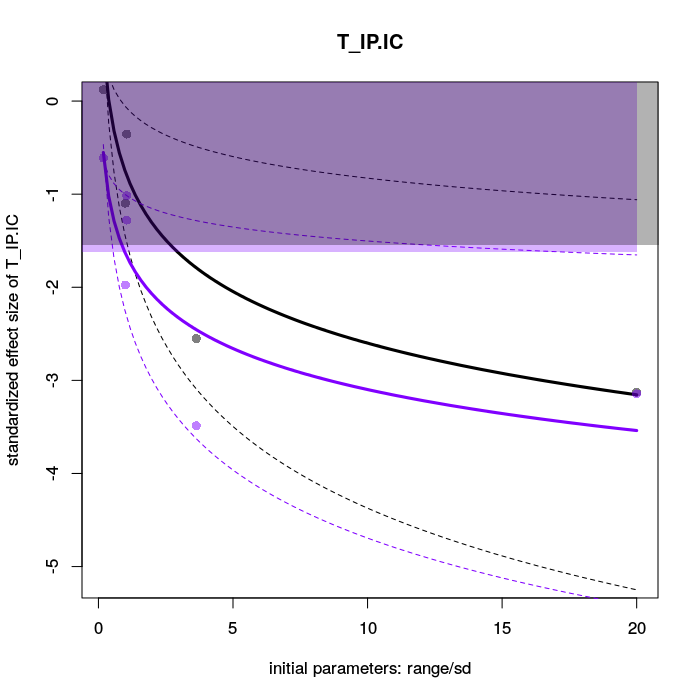
\includegraphics[width=\maxwidth]{figure/In_conc_plot-1} 

}

\caption[Power of $T_{IP/IC}$ to detect internal filtering]{Power of $T_{IP/IC}$ to detect internal filtering: Standardised Effect Size (SES) of $T_{IP/IC}$ in relation to the strength of internal filtering. Trait 'a' normally distributed is shown in black, traits 'b' uniformally distributed in purple. Open circle represent local SES values wheras close one represent global SES values. The exponential linear model is presented with 5 percents confidence interval on both side. Colored area represent the mean confidence interval of SES values ($alpha = 0.95$)\label{fig:In_conc_plot}}
\end{figure}


\end{knitrout}

\begin{knitrout}\small
\definecolor{shadecolor}{rgb}{0.969, 0.969, 0.969}\color{fgcolor}\begin{kframe}
\begin{alltt}
\hlstd{yy.norm} \hlkwb{<-} \hlkwd{mean}\hlstd{(}\hlkwd{c}\hlstd{(SES.inf.MEAN.norm_Tipic, meanSES.INF_glob.norm_Tipic),} \hlkwc{na.rm} \hlstd{= T)}
\hlstd{yy.uni} \hlkwb{<-} \hlkwd{mean}\hlstd{(}\hlkwd{c}\hlstd{(SES.inf.MEAN.uni_Tipic, meanSES.INF_glob.uni_Tipic),} \hlkwc{na.rm} \hlstd{= T)}

\hlstd{param_beta0.05_Tipic.norm} \hlkwb{<-} \hlkwd{exp}\hlstd{((yy.norm} \hlopt{-} \hlstd{lm.norm_conf [}\hlnum{1}\hlstd{,} \hlnum{2}\hlstd{])} \hlopt{/} \hlstd{lm.norm_conf [}\hlnum{2}\hlstd{,} \hlnum{2}\hlstd{])}
\hlstd{param_beta0.05_Tipic.uni} \hlkwb{<-} \hlkwd{exp}\hlstd{((yy.uni} \hlopt{-} \hlstd{lm.uni_conf [}\hlnum{1}\hlstd{,} \hlnum{2}\hlstd{])} \hlopt{/} \hlstd{lm.uni_conf [}\hlnum{2}\hlstd{,} \hlnum{2}\hlstd{])}
\end{alltt}
\end{kframe}
\end{knitrout}


For the trait "a" normally distributed, the power of $T_{IP/IC}$ is satisfying if the ratio of the initial parameter is superior to
 1.05. For the trait "b" uniformally distributed, this value is 0.51. 
 Further investigation on real data with different strength of internal filtering are needed to complete these simulated values.

 

























\cleardoublepage

\section{External Filter}

 \subsection {Randomization outline}
 
As for internal filter we modulate the strength of the external filter thanks to two parameters:
we define (i) a gradient of range between communities means traits distributions and (ii) a gradient of the mean variance in communities traits distributions. We expect the external filtering to increase (i) when the range in communities means increase (\textit{i.e.} the environmental gradient is larger) and (ii) when the variance in the communities traits distributions decrease (\textit{i.e.} the environmental gradient is stronger).
\\

In analogy with the internal filtering model, we defined 10 values for two parameters:
\\

 (i) \texttt{param\_{}RANGE.init} is a vector of length 10 which defined the above range for the mean traits values (the maximum value for the mean is assessed to 250). In decreasing the range of traits values while keeping the same number of communities, there is a decrease in the overlap of the communities traits distributions and consequently an decrease of the impact of external filtering in shaping traits distributions. Thus the mean for each communities is drawing from a normal distribution with standard deviation of 10 (parameter \texttt{mean\_{}sd.param}) and means evenly
\footnote{In fact, we draw this values in a normal distribution with means evenly distributed and with a standard error equal to \texttt{mean\_{}sd.param}}
of 10 distributed between \texttt{max.value\_{}traits - param\_{}RANGE} and \texttt{max.value\_{}traits}.
\\

(ii) \texttt{param\_{}SD} is a vector of length 10 which defined the standard deviation of traits distributions for each species. In order to decorrelating the mean and standard deviation of species traits distributions, \texttt{param\_{}SD} is sample before the analysis. 
\\

 Thus for the trait "a" the trait value for each individual is drawing from a normal distribution with the mean depending of it community attribute. For the trait "b" the trait value for each individual is drawing from a uniform distribution with the range depending of it community attribute.
 
\begin{knitrout}\small
\definecolor{shadecolor}{rgb}{0.969, 0.969, 0.969}\color{fgcolor}\begin{kframe}
\begin{alltt}
\hlcom{# Parameter for the range of communities traits distributions}
\hlstd{param_range.init} \hlkwb{<-} \hlkwd{round}\hlstd{(}\hlkwd{sort}\hlstd{(}\hlkwd{seq}\hlstd{(}\hlnum{10}\hlstd{,} \hlnum{200}\hlstd{,} \hlkwc{length.out} \hlstd{= nb_param_val)),} \hlnum{2}\hlstd{)}
\hlstd{param_range} \hlkwb{<-} \hlkwd{rep}\hlstd{(param_range.init, N_repet_Param)}
\hlstd{mean_sd.param} \hlkwb{<-} \hlkwd{rep}\hlstd{(}\hlnum{10}\hlstd{, nperm)}

\hlcom{# Parameter for the variance in species mean trait values}
\hlstd{param_SD} \hlkwb{<-} \hlkwd{seq}\hlstd{(}\hlnum{10}\hlstd{,} \hlnum{100}\hlstd{,}\hlkwc{length.out} \hlstd{= nb_param_val)}
\hlstd{sd_mean.param} \hlkwb{<-} \hlkwd{sample} \hlstd{(}\hlkwd{rep}\hlstd{(param_SD, N_repet_Param),}
       \hlkwc{size} \hlstd{=} \hlkwd{length}\hlstd{(}\hlkwd{rep}\hlstd{(param_SD, N_repet_Param)),} \hlkwc{replace} \hlstd{= F)}
\hlstd{sd_sd.param} \hlkwb{<-} \hlkwd{rep}\hlstd{(}\hlnum{10}\hlstd{, nperm)}
\end{alltt}
\end{kframe}
\end{knitrout}


\begin{knitrout}\small
\definecolor{shadecolor}{rgb}{0.969, 0.969, 0.969}\color{fgcolor}\begin{kframe}
\begin{alltt}
\hlstd{nperm} \hlkwb{<-} \hlstd{N_repet_Param}\hlopt{*}\hlkwd{length}\hlstd{(param_SD)}

\hlstd{mean_range_com} \hlkwb{<-} \hlkwd{list}\hlstd{() ; sd.com_stock3} \hlkwb{<-} \hlkwd{list}\hlstd{() ; res.simu3} \hlkwb{<-} \hlkwd{list}\hlstd{()}
\hlstd{res.simu3.pval} \hlkwb{<-} \hlkwd{list}\hlstd{() ; res.simu.traits3} \hlkwb{<-} \hlkwd{list}\hlstd{()}

\hlkwa{for}\hlstd{(n} \hlkwa{in} \hlnum{1}\hlopt{:}\hlstd{nperm)\{}\hlcom{#for each permutation}

 \hlstd{ex.sp3} \hlkwb{<-} \hlkwd{c}\hlstd{()}
 \hlstd{ex.com3} \hlkwb{<-} \hlkwd{matrix}\hlstd{(}\hlnum{0}\hlstd{,} \hlkwc{nrow} \hlstd{=} \hlnum{10}\hlstd{,} \hlkwc{ncol} \hlstd{=} \hlnum{20}\hlstd{)}
 \hlkwa{for}\hlstd{(i} \hlkwa{in} \hlnum{1}\hlopt{:} \hlnum{10}\hlstd{)\{}
  \hlstd{ex.com.interm} \hlkwb{<-} \hlkwd{table}\hlstd{(}\hlkwd{sample}\hlstd{(sp,} \hlkwc{size} \hlstd{=} \hlnum{100}\hlstd{,} \hlkwc{prob} \hlstd{=} \hlkwd{rlnorm}\hlstd{(}\hlnum{20}\hlstd{,} \hlnum{0}\hlstd{, sdlog),} \hlkwc{replace} \hlstd{= T))}
  \hlstd{ex.com3[i, sp}\hlopt \hlkwd{names}\hlstd{(ex.com.interm)]} \hlkwb{<-} \hlstd{ex.com.interm}
  \hlstd{ex.sp3} \hlkwb{<-} \hlkwd{c}\hlstd{(ex.sp3,} \hlkwd{rep}\hlstd{(sp,} \hlkwc{times} \hlstd{= ex.com3[i,]))}
 \hlstd{\}}

 \hlstd{ex.indplot3} \hlkwb{<-} \hlkwd{as.factor}\hlstd{(}\hlkwd{rep}\hlstd{(com,} \hlnum{100}\hlstd{))}

 \hlcom{#Defining mean and sd by community}
 \hlstd{mean_mean.param.interm} \hlkwb{<-} \hlkwd{seq}\hlstd{(max.value_traits} \hlopt{-} \hlstd{param_range[n], max.value_traits,}
                               \hlkwc{length.out} \hlstd{=} \hlkwd{length}\hlstd{(}\hlkwd{unique}\hlstd{(param_range)))}

 \hlstd{mean_mean.param} \hlkwb{<-} \hlkwd{rep}\hlstd{(}\hlkwd{round}\hlstd{(}\hlkwd{sort}\hlstd{(mean_mean.param.interm),} \hlnum{2}\hlstd{), N_repet_Param)}

 \hlstd{mean.com} \hlkwb{<-} \hlkwd{rnorm}\hlstd{(}\hlkwd{length}\hlstd{(}\hlkwd{unique}\hlstd{(com)),} \hlkwc{mean} \hlstd{= mean_mean.param,} \hlkwc{sd} \hlstd{= mean_sd.param[n])}
 \hlstd{sd.com} \hlkwb{<-} \hlkwd{rnorm}\hlstd{(}\hlkwd{length}\hlstd{(}\hlkwd{unique}\hlstd{(com)),} \hlkwc{mean} \hlstd{= sd_mean.param[n],} \hlkwc{sd} \hlstd{= sd_sd.param[n])}

 \hlstd{ex.traits3} \hlkwb{<-} \hlkwd{array}\hlstd{(}\hlnum{NA}\hlstd{,} \hlkwc{dim} \hlstd{=} \hlkwd{c}\hlstd{(}\hlnum{1000}\hlstd{,} \hlnum{2}\hlstd{))}
 \hlkwd{colnames}\hlstd{(ex.traits3)} \hlkwb{<-} \hlkwd{paste}\hlstd{(}\hlstr{"trait"}\hlstd{,} \hlkwd{c}\hlstd{(}\hlstr{"a"}\hlstd{,} \hlstr{"b"}\hlstd{),} \hlkwc{sep} \hlstd{=} \hlstr{" "}\hlstd{)}


 \hlkwa{for}\hlstd{(c} \hlkwa{in} \hlkwd{unique}\hlstd{(ex.indplot3))\{}
  \hlcom{#trait a : normal distribution}
  \hlstd{ex.traits3[ex.indplot3} \hlopt{==} \hlstd{c,} \hlnum{1}\hlstd{]} \hlkwb{<-}
  \hlkwd{rnorm}\hlstd{(}\hlnum{500}\hlstd{,} \hlkwd{rep}\hlstd{(mean.com[}\hlkwd{unique}\hlstd{(ex.indplot3)} \hlopt{==} \hlstd{c],} \hlnum{500}\hlstd{),}
    \hlkwd{rep}\hlstd{(sd.com[}\hlkwd{unique}\hlstd{(ex.indplot3)} \hlopt{==} \hlstd{c],} \hlnum{500}\hlstd{))[}\hlnum{1}\hlopt{:}\hlkwd{sum}\hlstd{(ex.indplot3} \hlopt{==} \hlstd{c)]}

  \hlcom{#trait b : uniform distribution}
  \hlstd{ex.traits3[ex.indplot3} \hlopt{==} \hlstd{c,} \hlnum{2}\hlstd{]} \hlkwb{<-}
  \hlkwd{runif}\hlstd{(}\hlnum{500}\hlstd{,} \hlkwc{min} \hlstd{=} \hlkwd{rep}\hlstd{(mean.com[}\hlkwd{unique}\hlstd{(ex.indplot3)} \hlopt{==} \hlstd{c],} \hlnum{500}\hlstd{)} \hlopt{-}
        \hlkwd{rep}\hlstd{(sd.com[}\hlkwd{unique}\hlstd{(ex.indplot3)} \hlopt{==} \hlstd{c],} \hlnum{500}\hlstd{),}
        \hlkwc{max} \hlstd{=} \hlkwd{rep}\hlstd{(mean.com[}\hlkwd{unique}\hlstd{(ex.indplot3)} \hlopt{==} \hlstd{c],} \hlnum{500}\hlstd{)} \hlopt{+}
        \hlkwd{rep}\hlstd{(sd.com[}\hlkwd{unique}\hlstd{(ex.indplot3)} \hlopt{==} \hlstd{c],} \hlnum{500}\hlstd{))[}\hlnum{1}\hlopt{:}\hlkwd{sum}\hlstd{(ex.indplot3} \hlopt{==} \hlstd{c)]}
 \hlstd{\}}

 \hlcom{#stock results}
 \hlstd{mean_range_com[[n]]} \hlkwb{<-} \hlkwd{c}\hlstd{(}\hlkwd{max}\hlstd{(ex.traits3[,} \hlnum{1}\hlstd{],} \hlkwc{na.rm} \hlstd{= T)} \hlopt{-} \hlkwd{min}\hlstd{(ex.traits3[,} \hlnum{1}\hlstd{],} \hlkwc{na.rm} \hlstd{= T),}
                          \hlkwd{max}\hlstd{(ex.traits3[,} \hlnum{2}\hlstd{],} \hlkwc{na.rm} \hlstd{= T)} \hlopt{-} \hlkwd{min}\hlstd{(ex.traits3[,} \hlnum{2}\hlstd{],} \hlkwc{na.rm} \hlstd{= T))}
 \hlstd{sd.com_stock3[[n]]} \hlkwb{<-} \hlstd{sd.com}

 \hlstd{res.simu.traits3[[n]]} \hlkwb{<-} \hlstd{ex.traits3}
 \hlstd{res.simu3[[n]]} \hlkwb{<-} \hlkwd{Tstats}\hlstd{(ex.traits3, ex.indplot3, ex.sp3)}
 \hlstd{res.simu3.pval[[n]]} \hlkwb{<-} \hlkwd{sum_Tstats}\hlstd{(res.simu3[[n]],} \hlkwc{type} \hlstd{=} \hlstr{"p.value"}\hlstd{)}
 \hlkwd{print}\hlstd{(}\hlkwd{paste}\hlstd{(}\hlstr{"---"}\hlstd{,} \hlkwd{round}\hlstd{(n}\hlopt{/}\hlstd{nperm,} \hlnum{2}\hlstd{)} \hlopt{*} \hlnum{100}\hlstd{,} \hlstr{"%"}\hlstd{,} \hlkwc{sep} \hlstd{=} \hlstr{" "}\hlstd{))}
\hlstd{\}}\hlcom{#end of simulation}
\end{alltt}
\end{kframe}
\end{knitrout}

 \subsection {Results for simulations of external filtering}

Let's see the result for one typical randomization. We can plot the distribution of traits within species and/or communities thanks to the function \texttt{plotDistri} (Fig. \ref{fig:typical_results_external_filtering1}). 

\begin{knitrout}\small
\definecolor{shadecolor}{rgb}{0.969, 0.969, 0.969}\color{fgcolor}\begin{kframe}
\begin{alltt}
\hlkwd{par}\hlstd{(}\hlkwc{mfrow}\hlstd{=}\hlkwd{c}\hlstd{(}\hlnum{2}\hlstd{,} \hlnum{2}\hlstd{))}
\hlkwd{plotDistri}\hlstd{(ex.traits3,} \hlkwd{rep}\hlstd{(}\hlstr{"all_sp"}\hlstd{,} \hlkwc{times} \hlstd{=} \hlkwd{dim}\hlstd{(ex.traits3)[}\hlnum{1}\hlstd{]), ex.indplot3,}
           \hlkwc{plot.ask} \hlstd{= F,} \hlkwc{multipanel} \hlstd{= F,} \hlkwc{main} \hlstd{=} \hlkwd{c}\hlstd{(}\hlstr{"a"}\hlstd{,} \hlstr{"b"}\hlstd{),} \hlkwc{leg} \hlstd{=} \hlkwd{c}\hlstd{(T, F))}
\hlkwd{plotDistri}\hlstd{(ex.traits3,} \hlkwd{rep}\hlstd{(}\hlstr{"region"}\hlstd{,} \hlkwc{times} \hlstd{=} \hlkwd{dim}\hlstd{(ex.traits3)[}\hlnum{1}\hlstd{]), ex.sp3,} \hlkwc{plot.ask} \hlstd{= F,}
           \hlkwc{multipanel} \hlstd{= F,} \hlkwc{main} \hlstd{=} \hlkwd{c}\hlstd{(}\hlstr{"c"}\hlstd{,} \hlstr{"d"}\hlstd{),} \hlkwc{leg} \hlstd{=} \hlkwd{c}\hlstd{(T, F))}
\hlkwd{par}\hlstd{(}\hlkwc{mfrow}\hlstd{=}\hlkwd{c}\hlstd{(}\hlnum{1}\hlstd{,} \hlnum{1}\hlstd{))}
\end{alltt}
\end{kframe}\begin{figure}

{\centering 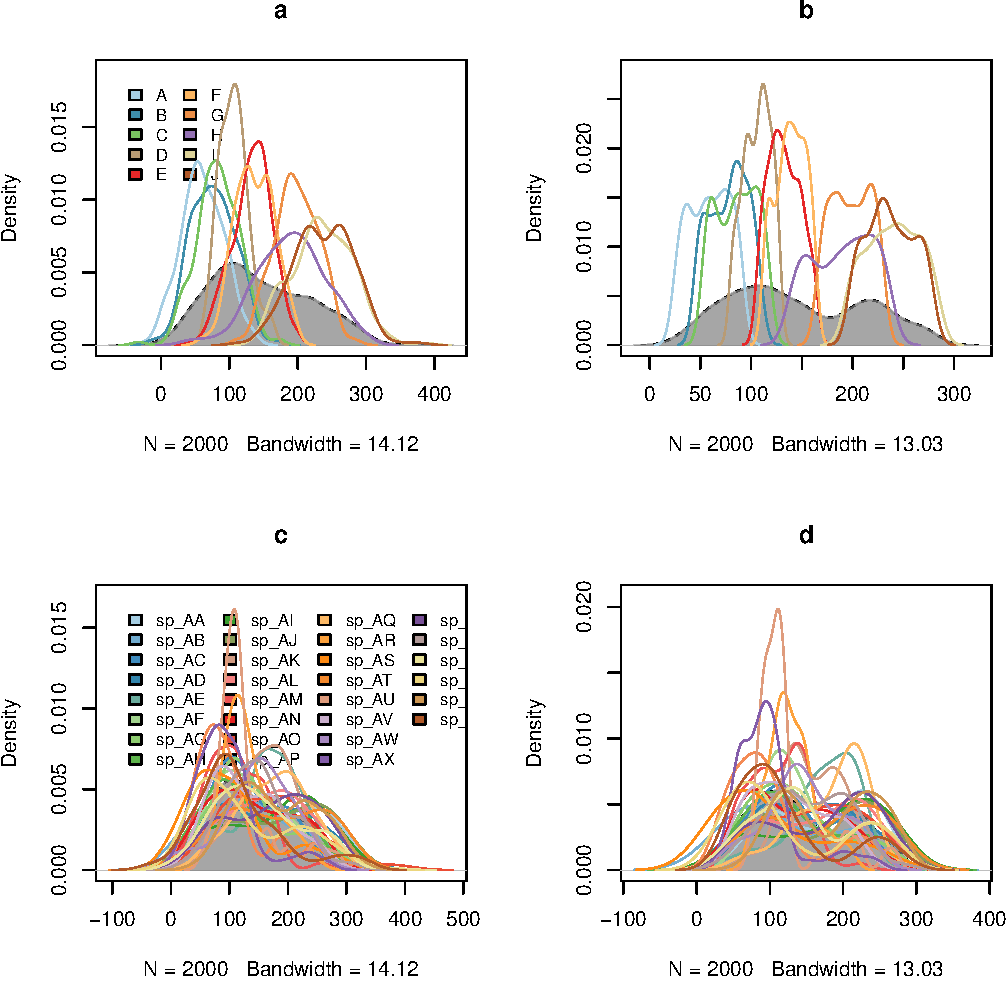
\includegraphics[width=\maxwidth]{figure/typical_results_external_filtering1-1} 

}

\caption[Distribution of traits for one randomization with external filter]{Distribution of traits for one randomization with external filter: (a) Communities trait distributions for the trait a (normal distribution); (b) Communities trait distributions for the trait b (uniform distribution); (c) Species trait distributions for the trait a; (d) Species trait distributions for the trait b\label{fig:typical_results_external_filtering1}}
\end{figure}


\end{knitrout}

We can also plot the result of the T-statistics for two contrasting case (Fig. \ref{fig:typical_results_external_filtering2}).

\begin{knitrout}\small
\definecolor{shadecolor}{rgb}{0.969, 0.969, 0.969}\color{fgcolor}\begin{kframe}
\begin{alltt}
\hlkwd{par}\hlstd{(}\hlkwc{mfrow}\hlstd{=}\hlkwd{c}\hlstd{(}\hlnum{2}\hlstd{,} \hlnum{1}\hlstd{))}
\hlkwd{plot}\hlstd{(res.simu3[[}\hlnum{1}\hlstd{]],} \hlkwc{main} \hlstd{=} \hlstr{"a"}\hlstd{)}
\hlkwd{plot}\hlstd{(res.simu3[[n]],} \hlkwc{main} \hlstd{=} \hlstr{"b"}\hlstd{)}
\hlkwd{par}\hlstd{(}\hlkwc{mfrow}\hlstd{=}\hlkwd{c}\hlstd{(}\hlnum{1}\hlstd{,} \hlnum{1}\hlstd{))}
\end{alltt}
\end{kframe}\begin{figure}

{\centering 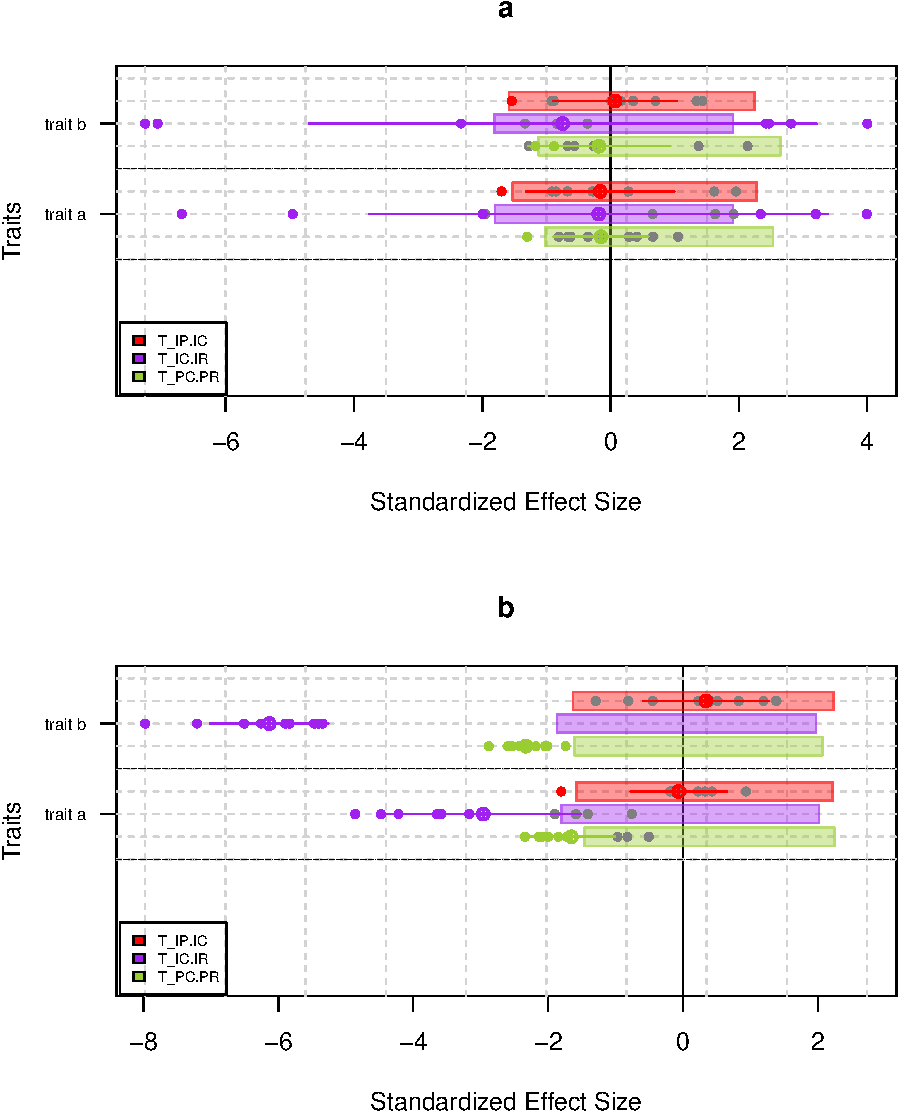
\includegraphics[width=\maxwidth]{figure/typical_results_external_filtering2-1} 

}

\caption[Results of T-statistics of traits for two randomization with contrasted strength of external filter]{Results of T-statistics of traits for two randomization with contrasted strength of external filter: $T_{IP/IC}$ in red, $T_{IC/IR}$ in purple and $T_{PC/PR}$ in green. (a) Lower strength of external filtering and (b) higher strength of external filtering.\label{fig:typical_results_external_filtering2}}
\end{figure}


\end{knitrout}

 \subsubsection {Local $T_{IC/IR}$ and $T_{PC/PR}$ results}

As for internal filtering, we mingle the p-value for different parameters values. Consequently we plot the standard effect size (SES) of $T_{IC/IR}$ and $T_{PC/PR}$ in relation to the initial parameters values. 

  \subsubsubsection {Local $T_{IC/IR}$ and $T_{PC/PR}$ SES values against initial parameter values}

\begin{knitrout}\small
\definecolor{shadecolor}{rgb}{0.969, 0.969, 0.969}\color{fgcolor}\begin{kframe}
\begin{alltt}
\hlcom{#T_IC.IR}
\hlstd{meanSES.3loc.norm_Ticir} \hlkwb{<-} \hlkwd{unlist}\hlstd{(}\hlkwd{lapply}\hlstd{(res.simu3,} \hlkwa{function}\hlstd{(}\hlkwc{x}\hlstd{)}
             \hlkwd{ses.listofindex}\hlstd{(}\hlkwd{as.listofindex}\hlstd{(x))}
             \hlopt{$}\hlstd{index_1_2}\hlopt{$}\hlstd{ses[,} \hlnum{1}\hlstd{]))}

\hlstd{meanSES.3loc.uni_Ticir} \hlkwb{<-} \hlkwd{unlist}\hlstd{(}\hlkwd{lapply}\hlstd{(res.simu3,} \hlkwa{function}\hlstd{(}\hlkwc{x}\hlstd{)}
             \hlkwd{ses.listofindex}\hlstd{(}\hlkwd{as.listofindex}\hlstd{(x))}
             \hlopt{$}\hlstd{index_1_2}\hlopt{$}\hlstd{ses[,} \hlnum{2}\hlstd{]))}

\hlstd{SES.inf.MEAN.norm_Ticir} \hlkwb{<-} \hlkwd{unlist}\hlstd{(}\hlkwd{lapply}\hlstd{(res.simu3,} \hlkwa{function}\hlstd{(}\hlkwc{x}\hlstd{)}
             \hlkwd{ses.listofindex}\hlstd{(}\hlkwd{as.listofindex}\hlstd{(x))}
             \hlopt{$}\hlstd{index_1_2}\hlopt{$}\hlstd{ses.inf[,} \hlnum{1}\hlstd{]))}

\hlstd{SES.inf.MEAN.uni_Ticir} \hlkwb{<-} \hlkwd{unlist}\hlstd{(}\hlkwd{lapply}\hlstd{(res.simu3,} \hlkwa{function}\hlstd{(}\hlkwc{x}\hlstd{)}
             \hlkwd{ses.listofindex}\hlstd{(}\hlkwd{as.listofindex}\hlstd{(x))}
             \hlopt{$}\hlstd{index_1_2}\hlopt{$}\hlstd{ses.inf[,} \hlnum{2}\hlstd{]))}

\hlcom{#T_PC.PR}
\hlstd{meanSES.3loc.norm_Tpcpr} \hlkwb{<-} \hlkwd{unlist}\hlstd{(}\hlkwd{lapply}\hlstd{(res.simu3,} \hlkwa{function}\hlstd{(}\hlkwc{x}\hlstd{)}
             \hlkwd{ses.listofindex}\hlstd{(}\hlkwd{as.listofindex}\hlstd{(x))}
             \hlopt{$}\hlstd{index_1_3}\hlopt{$}\hlstd{ses[,} \hlnum{1}\hlstd{]))}

\hlstd{meanSES.3loc.uni_Tpcpr} \hlkwb{<-} \hlkwd{unlist}\hlstd{(}\hlkwd{lapply}\hlstd{(res.simu3,} \hlkwa{function}\hlstd{(}\hlkwc{x}\hlstd{)}
             \hlkwd{ses.listofindex}\hlstd{(}\hlkwd{as.listofindex}\hlstd{(x))}
             \hlopt{$}\hlstd{index_1_3}\hlopt{$}\hlstd{ses[,} \hlnum{2}\hlstd{]))}

\hlstd{SES.inf.MEAN.norm_Tpcpr} \hlkwb{<-} \hlkwd{unlist}\hlstd{(}\hlkwd{lapply}\hlstd{(res.simu3,} \hlkwa{function}\hlstd{(}\hlkwc{x}\hlstd{)}
             \hlkwd{ses.listofindex}\hlstd{(}\hlkwd{as.listofindex}\hlstd{(x))}
             \hlopt{$}\hlstd{index_1_3}\hlopt{$}\hlstd{ses.inf[,} \hlnum{1}\hlstd{]))}

\hlstd{SES.inf.MEAN.uni_Tpcpr} \hlkwb{<-} \hlkwd{unlist}\hlstd{(}\hlkwd{lapply}\hlstd{(res.simu3,} \hlkwa{function}\hlstd{(}\hlkwc{x}\hlstd{)}
             \hlkwd{ses.listofindex}\hlstd{(}\hlkwd{as.listofindex}\hlstd{(x))}
             \hlopt{$}\hlstd{index_1_3}\hlopt{$}\hlstd{ses.inf[,} \hlnum{2}\hlstd{]))}
\end{alltt}
\end{kframe}
\end{knitrout}

Now, we can plot SES of $T_{IC/IR}$ (Fig. \ref{fig:Ex_filter_results_plot_initparam1}) and $T_{PC/PR}$ (Fig. \ref{fig:Ex_filter_results_plot_initparam2}). The trait "a" normally distributed is in black and the uniform traits "b" is in purple. The colored rectangles represent the null model area with alpha = 5\%. Thus, when a point is outside these area, the modeled parameters are strong enough to detect the external filter with a high power (beta-error $ < 0.05$).

\begin{knitrout}\small
\definecolor{shadecolor}{rgb}{0.969, 0.969, 0.969}\color{fgcolor}\begin{kframe}
\begin{alltt}
\hlstd{init_param} \hlkwb{<-} \hlstd{param_range} \hlopt{/} \hlstd{sd_mean.param}
\hlcom{#each value is replicate Ncom times (there is Ncom communities for each parameter values)}
\hlstd{init_param.loc} \hlkwb{<-} \hlkwd{rep}\hlstd{(init_param,} \hlkwc{each} \hlstd{= Ncom)}

\hlkwd{plot}\hlstd{(meanSES.3loc.norm_Ticir, init_param.loc,} \hlkwc{pch} \hlstd{=} \hlnum{16}\hlstd{,} \hlkwc{col} \hlstd{=} \hlkwd{rgb}\hlstd{(}\hlnum{0}\hlstd{,} \hlnum{0}\hlstd{,} \hlnum{0}\hlstd{,} \hlnum{0.6}\hlstd{),}
     \hlkwc{xlim} \hlstd{=} \hlkwd{c}\hlstd{(}\hlkwd{min}\hlstd{(}\hlkwd{c}\hlstd{(}\hlkwd{unlist}\hlstd{(meanSES.3loc.norm_Ticir),} \hlkwd{unlist}\hlstd{(meanSES.3loc.uni_Ticir)),}
     \hlkwc{na.rm} \hlstd{= T),} \hlnum{0}\hlstd{),}
     \hlkwc{main} \hlstd{=} \hlstr{"Local T_IC.IR"}\hlstd{,}
     \hlkwc{xlab} \hlstd{=} \hlstr{"standardized effect size of T_IC.IR"}\hlstd{,}
     \hlkwc{ylab} \hlstd{=} \hlstr{"initial parameters: range/sd"}\hlstd{)}
\hlkwd{abline}\hlstd{(}\hlkwc{v} \hlstd{=} \hlkwd{mean}\hlstd{(SES.inf.MEAN.norm_Ticir,} \hlkwc{na.rm} \hlstd{= T))}

\hlkwd{points}\hlstd{(meanSES.3loc.uni_Ticir, init_param.loc,} \hlkwc{pch} \hlstd{=} \hlnum{16}\hlstd{,} \hlkwc{col} \hlstd{=} \hlkwd{rgb}\hlstd{(}\hlnum{0.5}\hlstd{,} \hlnum{0}\hlstd{,} \hlnum{1}\hlstd{,} \hlnum{0.6}\hlstd{))}
\hlkwd{abline}\hlstd{(}\hlkwc{v} \hlstd{=} \hlkwd{mean}\hlstd{(SES.inf.MEAN.uni_Ticir,} \hlkwc{na.rm} \hlstd{= T),} \hlkwc{col} \hlstd{=} \hlstr{"purple"}\hlstd{)}
\hlkwd{rect}\hlstd{(}\hlkwd{mean}\hlstd{(SES.inf.MEAN.norm_Ticir,} \hlkwc{na.rm} \hlstd{= T),} \hlopt{-}\hlnum{1}\hlstd{,} \hlnum{0}\hlstd{,} \hlkwd{max}\hlstd{(init_param)} \hlopt{+} \hlnum{1}\hlstd{,}
     \hlkwc{col} \hlstd{=} \hlkwd{rgb}\hlstd{(}\hlnum{0}\hlstd{,} \hlnum{0}\hlstd{,} \hlnum{0}\hlstd{,} \hlnum{0.3}\hlstd{),} \hlkwc{border} \hlstd{=} \hlnum{NA}\hlstd{)}
\hlkwd{rect}\hlstd{(}\hlkwd{mean}\hlstd{(SES.inf.MEAN.uni_Ticir,} \hlkwc{na.rm} \hlstd{= T),}\hlnum{0}\hlstd{,} \hlnum{0}\hlstd{,} \hlkwd{max}\hlstd{(init_param),}
     \hlkwc{col} \hlstd{=} \hlkwd{rgb}\hlstd{(}\hlnum{0.5}\hlstd{,} \hlnum{0}\hlstd{,} \hlnum{1}\hlstd{,} \hlnum{0.3}\hlstd{),} \hlkwc{border} \hlstd{=} \hlnum{NA}\hlstd{)}
\end{alltt}
\end{kframe}\begin{figure}

{\centering 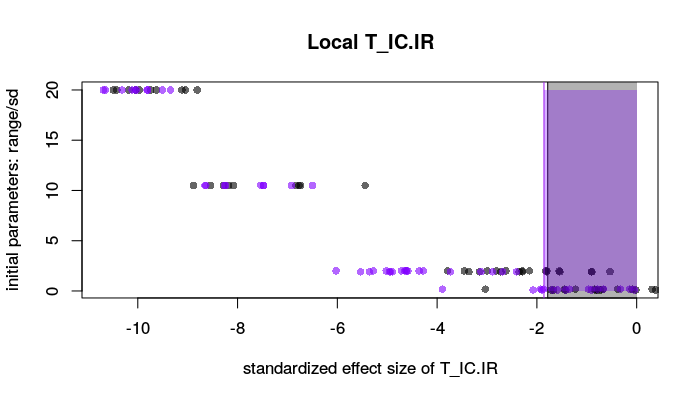
\includegraphics[width=\maxwidth]{figure/Ex_filter_results_plot_initparam1-1} 

}

\caption[Local $T_{IC/IR}$ SES and initial parameters values]{Local $T_{IC/IR}$ SES and initial parameters values: Standardized effect size of $T_{IC/IR}$ in function of the strength of external filter defined by the ratio of the initial range parameter by the initial standard error parameter. Colored area represent the mean confidence interval of SES values ($alpha = 0.95$). Trait a (normal) in black and b (uniform) in purple.\label{fig:Ex_filter_results_plot_initparam1}}
\end{figure}


\end{knitrout}
 
  
\begin{knitrout}\small
\definecolor{shadecolor}{rgb}{0.969, 0.969, 0.969}\color{fgcolor}\begin{kframe}
\begin{alltt}
\hlkwd{plot}\hlstd{(meanSES.3loc.norm_Tpcpr, init_param.loc,} \hlkwc{pch} \hlstd{=} \hlnum{16}\hlstd{,} \hlkwc{col} \hlstd{=} \hlkwd{rgb}\hlstd{(}\hlnum{0}\hlstd{,} \hlnum{0}\hlstd{,} \hlnum{0}\hlstd{,} \hlnum{0.6}\hlstd{),}
     \hlkwc{xlim} \hlstd{=} \hlkwd{c}\hlstd{(}\hlkwd{min}\hlstd{(}\hlkwd{c}\hlstd{(}\hlkwd{unlist}\hlstd{(meanSES.3loc.norm_Tpcpr),} \hlkwd{unlist}\hlstd{(meanSES.3loc.uni_Tpcpr)),}
     \hlkwc{na.rm} \hlstd{= T),} \hlnum{0}\hlstd{),}
     \hlkwc{main} \hlstd{=} \hlstr{"Local T_PC.PR"}\hlstd{,}
     \hlkwc{xlab} \hlstd{=} \hlstr{"standardized effect size of T_PC.PR"}\hlstd{,}
     \hlkwc{ylab} \hlstd{=} \hlstr{"initial parameters: range/sd"}\hlstd{)}
\hlkwd{abline}\hlstd{(}\hlkwc{v} \hlstd{=} \hlkwd{mean}\hlstd{(SES.inf.MEAN.norm_Tpcpr,} \hlkwc{na.rm} \hlstd{= T))}

\hlkwd{points}\hlstd{(meanSES.3loc.uni_Tpcpr, init_param.loc,} \hlkwc{pch} \hlstd{=} \hlnum{16}\hlstd{,} \hlkwc{col} \hlstd{=} \hlkwd{rgb}\hlstd{(}\hlnum{0.5}\hlstd{,} \hlnum{0}\hlstd{,} \hlnum{1}\hlstd{,} \hlnum{0.6}\hlstd{))}
\hlkwd{abline}\hlstd{(}\hlkwc{v} \hlstd{=} \hlkwd{mean}\hlstd{(SES.inf.MEAN.uni_Tpcpr,} \hlkwc{na.rm} \hlstd{= T),} \hlkwc{col} \hlstd{=} \hlstr{"purple"}\hlstd{)}
\hlkwd{rect}\hlstd{(}\hlkwd{mean}\hlstd{(SES.inf.MEAN.norm_Tpcpr,} \hlkwc{na.rm} \hlstd{= T),} \hlopt{-}\hlnum{1}\hlstd{,} \hlnum{0}\hlstd{,} \hlkwd{max}\hlstd{(init_param)} \hlopt{+} \hlnum{1}\hlstd{,}
     \hlkwc{col} \hlstd{=} \hlkwd{rgb}\hlstd{(}\hlnum{0}\hlstd{,} \hlnum{0}\hlstd{,} \hlnum{0}\hlstd{,} \hlnum{0.3}\hlstd{),} \hlkwc{border} \hlstd{=} \hlnum{NA}\hlstd{)}
\hlkwd{rect}\hlstd{(}\hlkwd{mean}\hlstd{(SES.inf.MEAN.uni_Tpcpr,} \hlkwc{na.rm} \hlstd{= T),} \hlnum{0}\hlstd{,} \hlnum{0}\hlstd{,} \hlkwd{max}\hlstd{(init_param),}
     \hlkwc{col} \hlstd{=} \hlkwd{rgb}\hlstd{(}\hlnum{0.5}\hlstd{,} \hlnum{0}\hlstd{,} \hlnum{1}\hlstd{,} \hlnum{0.3}\hlstd{),} \hlkwc{border} \hlstd{=} \hlnum{NA}\hlstd{)}
\end{alltt}
\end{kframe}\begin{figure}

{\centering 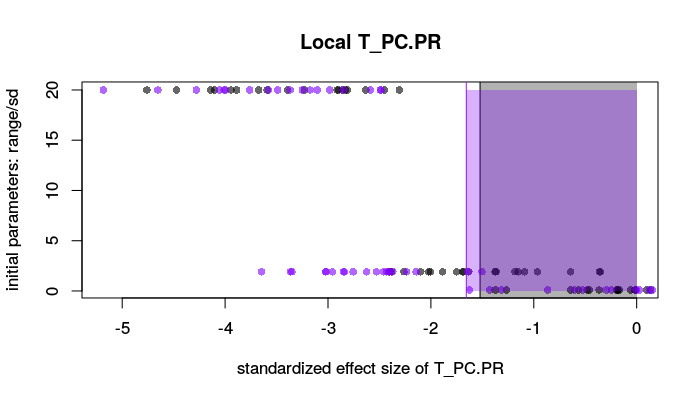
\includegraphics[width=\maxwidth]{figure/Ex_filter_results_plot_initparam2-1} 

}

\caption[Local $T_{PC/PR}$ SES and initial parameters values]{Local $T_{PC/PR}$ SES and initial parameters values: Standardized effect size of $T_{PC/PR}$ in function of the strength of external filter defined by the ratio of the initial range parameter by the initial standard error parameter. Colored area represent the mean confidence interval of SES values ($alpha = 0.95$). Trait a (normal) in black and b (uniform) in purple.\label{fig:Ex_filter_results_plot_initparam2}}
\end{figure}


\end{knitrout}
 
For each initial parameters values we can calculate the proportion of case where we do not reject the null hypothesis while this hypothesis is wrong (\textit{i.e.} the Beta-error). The next chunk only show the calculation for the $T_{IC/IR}$ metrics on the trait "a".

\begin{knitrout}\small
\definecolor{shadecolor}{rgb}{0.969, 0.969, 0.969}\color{fgcolor}\begin{kframe}
\begin{alltt}
\hlstd{beta_range_norm_Ticir} \hlkwb{<-}
 \hlstd{(}\hlkwd{unlist}\hlstd{(}\hlkwd{lapply}\hlstd{(}\hlkwd{by}\hlstd{(}\hlkwd{cbind}\hlstd{(meanSES.3loc.norm_Ticir, SES.inf.MEAN.norm_Ticir),}
     \hlkwd{rep}\hlstd{(param_range,} \hlkwc{each} \hlstd{= Ncom),} \hlkwa{function}\hlstd{(}\hlkwc{x}\hlstd{) x[,}\hlnum{1}\hlstd{]} \hlopt{>} \hlstd{x[,}\hlnum{2}\hlstd{]),}
     \hlkwa{function}\hlstd{(}\hlkwc{x}\hlstd{)} \hlkwd{sum}\hlstd{(x,} \hlkwc{na.rm} \hlstd{= T)))}\hlopt{+}\hlnum{1}\hlstd{)}\hlopt{/}\hlstd{(}\hlnum{10} \hlopt{*} \hlstd{N_repet_Param} \hlopt{+} \hlnum{1}\hlstd{)}
\end{alltt}
\end{kframe}
\end{knitrout}

\begin{kframe}
\begin{alltt}
\hlkwd{print}\hlstd{(}\hlkwd{xtable}\hlstd{(res_beta_Ticir,} \hlkwc{caption} \hlstd{=} \hlstr{'Local beta-error of $T_\{IC/IR\}$ in function 
             of the strength of external filtering. str: strength. Trait a is 
             normally distributed and trait b is uniformally distributed.'}\hlstd{,}
             \hlkwc{label} \hlstd{=} \hlstr{"tab:local_beta_error_xtable_ticir"}\hlstd{),}
      \hlkwc{caption.placement} \hlstd{=} \hlstr{"top"}\hlstd{,} \hlkwc{size} \hlstd{=} \hlstr{"small"}\hlstd{)}
\end{alltt}
\end{kframe}% latex table generated in R 3.1.2 by xtable 1.7-4 package
% Wed Jan 14 00:52:54 2015
\begin{table}[ht]
\centering
\caption{Local beta-error of $T_{IC/IR}$ in function 
             of the strength of external filtering. str: strength. Trait a is 
             normally distributed and trait b is uniformally distributed.} 
\label{tab:local_beta_error_xtable_ticir}
{\small
\begin{tabular}{rrrrrrrrrrr}
  \hline
 & str 1 & str 2 & str 3 & str 4 & str 5 & str 6 & str 7 & str 8 & str 9 & str 10 \\ 
  \hline
effect of sd (a) & 0.68 & 0.61 & 0.56 & 0.45 & 0.40 & 0.36 & 0.30 & 0.21 & 0.17 & 0.08 \\ 
  effect of sd (b) & 0.36 & 0.28 & 0.28 & 0.19 & 0.19 & 0.16 & 0.14 & 0.08 & 0.08 & 0.03 \\ 
  effect of range (a) & 0.66 & 0.60 & 0.58 & 0.48 & 0.44 & 0.36 & 0.26 & 0.23 & 0.14 & 0.09 \\ 
  effect of range (b) & 0.53 & 0.43 & 0.34 & 0.22 & 0.14 & 0.08 & 0.02 & 0.01 & 0.00 & 0.00 \\ 
   \hline
\end{tabular}
}
\end{table}


\begin{kframe}
\begin{alltt}
\hlkwd{print}\hlstd{(}\hlkwd{xtable}\hlstd{(res_beta_Ticir,} \hlkwc{caption} \hlstd{=} \hlstr{'Local beta-error of $T_\{PC/PR\}$ in function 
             of the strength of external filtering. str: strength. Trait a is 
             normally distributed and trait b is uniformally distributed.'}\hlstd{,}
             \hlkwc{label} \hlstd{=} \hlstr{"tab:local_beta_error_xtable_tpcpr"}\hlstd{),}
      \hlkwc{caption.placement} \hlstd{=} \hlstr{"top"}\hlstd{,} \hlkwc{size} \hlstd{=} \hlstr{"small"}\hlstd{)}
\end{alltt}
\end{kframe}% latex table generated in R 3.1.2 by xtable 1.7-4 package
% Wed Jan 14 00:52:54 2015
\begin{table}[ht]
\centering
\caption{Local beta-error of $T_{PC/PR}$ in function 
             of the strength of external filtering. str: strength. Trait a is 
             normally distributed and trait b is uniformally distributed.} 
\label{tab:local_beta_error_xtable_tpcpr}
{\small
\begin{tabular}{rrrrrrrrrrr}
  \hline
 & str 1 & str 2 & str 3 & str 4 & str 5 & str 6 & str 7 & str 8 & str 9 & str 10 \\ 
  \hline
effect of sd (a) & 0.68 & 0.61 & 0.56 & 0.45 & 0.40 & 0.36 & 0.30 & 0.21 & 0.17 & 0.08 \\ 
  effect of sd (b) & 0.36 & 0.28 & 0.28 & 0.19 & 0.19 & 0.16 & 0.14 & 0.08 & 0.08 & 0.03 \\ 
  effect of range (a) & 0.66 & 0.60 & 0.58 & 0.48 & 0.44 & 0.36 & 0.26 & 0.23 & 0.14 & 0.09 \\ 
  effect of range (b) & 0.53 & 0.43 & 0.34 & 0.22 & 0.14 & 0.08 & 0.02 & 0.01 & 0.00 & 0.00 \\ 
   \hline
\end{tabular}
}
\end{table}

 
Now we can see the beta-error for each strength (table \ref{tab:local_beta_error_xtable_ticir} and \ref{tab:local_beta_error_xtable_tpcpr}). A high value of range and a low value of standard error defined a high strength of filtering. For example, in the case of a trait normally distributed, the proportion of false negative is 67.57\% for the higher value of standard errors and thus for the lower strength of external filtering.
 
 
  \subsubsubsection {Local $T_{IC/IR}$ and $T_{PC/PR}$ SES values against modeled parameter values}
  
  First we need to calculate the modeled parameter values. Here again we calculate the strength of external filtering by dividing the range of values in communities by their standard error.
  
\begin{knitrout}\small
\definecolor{shadecolor}{rgb}{0.969, 0.969, 0.969}\color{fgcolor}\begin{kframe}
\begin{alltt}
\hlstd{mean_range_com.interm} \hlkwb{<-} \hlkwd{t}\hlstd{(}\hlkwd{matrix}\hlstd{(}\hlkwd{unlist}\hlstd{(}\hlkwd{lapply}\hlstd{(mean_range_com,} \hlkwa{function}\hlstd{(}\hlkwc{x}\hlstd{) x)),} \hlkwc{nrow} \hlstd{=} \hlnum{2}\hlstd{))}
\hlstd{mean_sd_of_com} \hlkwb{<-} \hlkwd{unlist}\hlstd{(}\hlkwd{lapply}\hlstd{(sd.com_stock3,} \hlkwa{function}\hlstd{(}\hlkwc{x}\hlstd{)} \hlkwd{mean}\hlstd{(x)))}

\hlstd{modeled_param_norm} \hlkwb{<-} \hlstd{mean_range_com.interm[,} \hlnum{1}\hlstd{]} \hlopt{/} \hlstd{mean_sd_of_com}
\hlstd{modeled_param_uni} \hlkwb{<-} \hlstd{mean_range_com.interm[,} \hlnum{2}\hlstd{]} \hlopt{/} \hlstd{mean_sd_of_com}
\hlstd{modeled_param_norm.loc} \hlkwb{<-} \hlkwd{rep}\hlstd{(modeled_param_norm,} \hlkwc{each} \hlstd{= Ncom)}
\hlstd{modeled_param_uni.loc} \hlkwb{<-} \hlkwd{rep}\hlstd{(modeled_param_uni,} \hlkwc{each} \hlstd{= Ncom)}
\end{alltt}
\end{kframe}
\end{knitrout}

\begin{knitrout}\small
\definecolor{shadecolor}{rgb}{0.969, 0.969, 0.969}\color{fgcolor}\begin{kframe}
\begin{alltt}
\hlkwd{plot}\hlstd{(meanSES.3loc.norm_Ticir, modeled_param_norm.loc,} \hlkwc{pch} \hlstd{=} \hlnum{16}\hlstd{,} \hlkwc{col} \hlstd{=} \hlkwd{rgb}\hlstd{(}\hlnum{0}\hlstd{,} \hlnum{0}\hlstd{,} \hlnum{0}\hlstd{,} \hlnum{0.6}\hlstd{),}
  \hlkwc{xlim} \hlstd{=} \hlkwd{c}\hlstd{(}\hlkwd{min}\hlstd{(}\hlkwd{c}\hlstd{(}\hlkwd{unlist}\hlstd{(meanSES.3loc.norm_Ticir),} \hlkwd{unlist}\hlstd{(meanSES.3loc.uni_Ticir)),}
    \hlkwc{na.rm} \hlstd{= T),} \hlnum{0}\hlstd{),}
    \hlkwc{ylim} \hlstd{=} \hlkwd{c}\hlstd{(}\hlnum{0}\hlstd{,} \hlkwd{min}\hlstd{(}\hlkwd{max}\hlstd{(}\hlkwd{c}\hlstd{(modeled_param_norm.loc, modeled_param_uni.loc),} \hlkwc{na.rm} \hlstd{= T),}
                    \hlnum{100}\hlstd{)),}  \hlkwc{main} \hlstd{=} \hlstr{"Local T_IC.IR"}\hlstd{,}
  \hlkwc{xlab} \hlstd{=} \hlstr{"standardized effect size of T_IC.IR"}\hlstd{,}
  \hlkwc{ylab} \hlstd{=} \hlstr{"modeled parameters: range/sd"}\hlstd{)}
\hlkwd{abline}\hlstd{(}\hlkwc{v} \hlstd{=} \hlkwd{mean}\hlstd{(SES.inf.MEAN.norm_Ticir,} \hlkwc{na.rm} \hlstd{= T))}

\hlkwd{points}\hlstd{(meanSES.3loc.uni_Ticir, modeled_param_uni.loc,} \hlkwc{pch} \hlstd{=} \hlnum{16}\hlstd{,} \hlkwc{col} \hlstd{=} \hlkwd{rgb}\hlstd{(}\hlnum{0.5}\hlstd{,} \hlnum{0}\hlstd{,} \hlnum{1}\hlstd{,} \hlnum{0.6}\hlstd{))}
\hlkwd{abline}\hlstd{(}\hlkwc{v} \hlstd{=} \hlkwd{mean}\hlstd{(SES.inf.MEAN.uni_Ticir,} \hlkwc{na.rm} \hlstd{= T),} \hlkwc{col} \hlstd{=} \hlstr{"purple"}\hlstd{)}

\hlkwd{rect}\hlstd{(}\hlkwd{mean}\hlstd{(SES.inf.MEAN.norm_Ticir,} \hlkwc{na.rm} \hlstd{= T),} \hlopt{-}\hlnum{1}\hlstd{,} \hlnum{0}\hlstd{,} \hlkwd{max}\hlstd{(modeled_param_norm.loc)} \hlopt{+} \hlnum{1}\hlstd{,}
     \hlkwc{col} \hlstd{=} \hlkwd{rgb}\hlstd{(}\hlnum{0}\hlstd{,} \hlnum{0}\hlstd{,} \hlnum{0}\hlstd{,} \hlnum{0.3}\hlstd{),} \hlkwc{border} \hlstd{=} \hlnum{NA}\hlstd{)}
\hlkwd{rect}\hlstd{(}\hlkwd{mean}\hlstd{(SES.inf.MEAN.uni_Ticir,} \hlkwc{na.rm} \hlstd{= T),}\hlnum{0}\hlstd{,} \hlnum{0}\hlstd{,} \hlkwd{max}\hlstd{(modeled_param_uni.loc),}
     \hlkwc{col} \hlstd{=} \hlkwd{rgb}\hlstd{(}\hlnum{0.5}\hlstd{,} \hlnum{0}\hlstd{,} \hlnum{1}\hlstd{,} \hlnum{0.3}\hlstd{),} \hlkwc{border} \hlstd{=} \hlnum{NA}\hlstd{)}
\end{alltt}
\end{kframe}\begin{figure}

{\centering 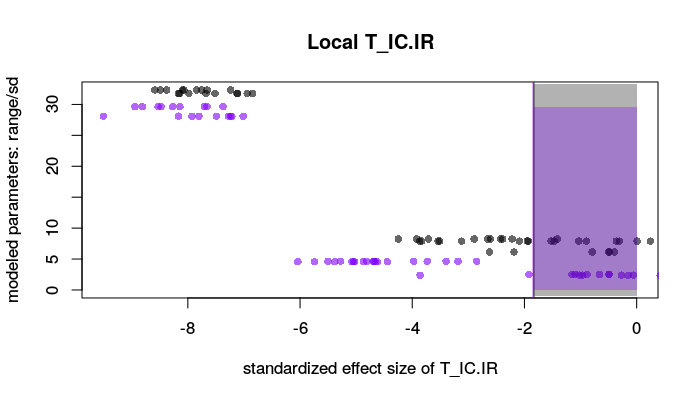
\includegraphics[width=\maxwidth]{figure/Ex_filter_results_plot_modeledparam1-1} 

}

\caption[Local $T_{IC/IR}$ SES and modeled parameters values]{Local $T_{IC/IR}$ SES and modeled parameters values: Standardized effect size of $T_{IC/IR}$ in function of the strength of external filter defined by the ratio of the modeled range parameter by the modeled standard error parameter. Colored area represent the mean confidence interval of SES values ($alpha = 0.95$). Trait a (normal) in black and b (uniform) in purple.\label{fig:Ex_filter_results_plot_modeledparam1}}
\end{figure}


\end{knitrout}

\begin{knitrout}\small
\definecolor{shadecolor}{rgb}{0.969, 0.969, 0.969}\color{fgcolor}\begin{kframe}
\begin{alltt}
\hlkwd{plot}\hlstd{(meanSES.3loc.norm_Tpcpr, modeled_param_norm.loc,} \hlkwc{pch} \hlstd{=} \hlnum{16}\hlstd{,} \hlkwc{col} \hlstd{=} \hlkwd{rgb}\hlstd{(}\hlnum{0}\hlstd{,} \hlnum{0}\hlstd{,} \hlnum{0}\hlstd{,} \hlnum{0.6}\hlstd{),}
     \hlkwc{xlim} \hlstd{=} \hlkwd{c}\hlstd{(}\hlkwd{min}\hlstd{(}\hlkwd{c}\hlstd{(}\hlkwd{unlist}\hlstd{(meanSES.3loc.norm_Tpcpr),} \hlkwd{unlist}\hlstd{(meanSES.3loc.uni_Tpcpr)),}
              \hlkwc{na.rm} \hlstd{= T),} \hlnum{0}\hlstd{),}
     \hlkwc{ylim} \hlstd{=} \hlkwd{c}\hlstd{(}\hlnum{0}\hlstd{,} \hlkwd{min}\hlstd{(}\hlkwd{max}\hlstd{(}\hlkwd{c}\hlstd{(modeled_param_norm.loc, modeled_param_uni.loc),} \hlkwc{na.rm} \hlstd{= T),}
                     \hlnum{100}\hlstd{)),}
     \hlkwc{main} \hlstd{=} \hlstr{"Local T_PC.PR"}\hlstd{,}
     \hlkwc{xlab} \hlstd{=} \hlstr{"standardized effect size of T_PC.PR"}\hlstd{,}
     \hlkwc{ylab} \hlstd{=} \hlstr{"modeled parameters: range/sd"}\hlstd{)}
\hlkwd{abline}\hlstd{(}\hlkwc{v} \hlstd{=} \hlkwd{mean}\hlstd{(SES.inf.MEAN.norm_Tpcpr,} \hlkwc{na.rm} \hlstd{= T))}

\hlkwd{points}\hlstd{(meanSES.3loc.uni_Tpcpr, modeled_param_uni.loc,} \hlkwc{pch} \hlstd{=} \hlnum{16}\hlstd{,} \hlkwc{col} \hlstd{=} \hlkwd{rgb}\hlstd{(}\hlnum{0.5}\hlstd{,} \hlnum{0}\hlstd{,} \hlnum{1}\hlstd{,} \hlnum{0.6}\hlstd{))}
\hlkwd{abline}\hlstd{(}\hlkwc{v} \hlstd{=} \hlkwd{mean}\hlstd{(SES.inf.MEAN.uni_Tpcpr,} \hlkwc{na.rm} \hlstd{= T),} \hlkwc{col} \hlstd{=} \hlstr{"purple"}\hlstd{)}
\hlkwd{rect}\hlstd{(}\hlkwd{mean}\hlstd{(SES.inf.MEAN.norm_Tpcpr,} \hlkwc{na.rm} \hlstd{= T),} \hlopt{-}\hlnum{1}\hlstd{,} \hlnum{0}\hlstd{,} \hlkwd{max}\hlstd{(modeled_param_norm.loc)} \hlopt{+} \hlnum{1}\hlstd{,}
     \hlkwc{col} \hlstd{=} \hlkwd{rgb}\hlstd{(}\hlnum{0}\hlstd{,} \hlnum{0}\hlstd{,} \hlnum{0}\hlstd{,} \hlnum{0.3}\hlstd{),} \hlkwc{border} \hlstd{=} \hlnum{NA}\hlstd{)}
\hlkwd{rect}\hlstd{(}\hlkwd{mean}\hlstd{(SES.inf.MEAN.uni_Tpcpr,} \hlkwc{na.rm} \hlstd{= T),} \hlnum{0}\hlstd{,} \hlnum{0}\hlstd{,} \hlkwd{max}\hlstd{(modeled_param_uni.loc),}
     \hlkwc{col} \hlstd{=} \hlkwd{rgb}\hlstd{(}\hlnum{0.5}\hlstd{,} \hlnum{0}\hlstd{,} \hlnum{1}\hlstd{,} \hlnum{0.3}\hlstd{),} \hlkwc{border} \hlstd{=} \hlnum{NA}\hlstd{)}
\end{alltt}
\end{kframe}\begin{figure}

{\centering 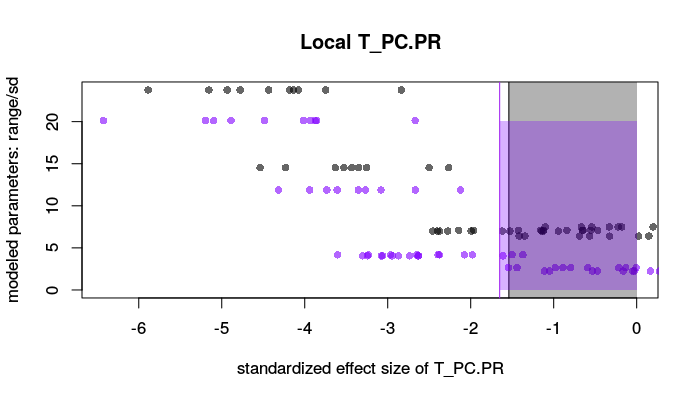
\includegraphics[width=\maxwidth]{figure/Ex_filter_results_plot_modeledparam2-1} 

}

\caption[Local $T_{PC/PR}$ SES and modeled parameters values]{Local $T_{PC/PR}$ SES and modeled parameters values: Standardized effect size of $T_{PC/PR}$ in function of the strength of external filter defined by the ratio of the modeled range parameter by the modeled standard error parameter. Colored area represent the mean confidence interval of SES values ($alpha = 0.95$). Trait a (normal) in black and b (uniform) in purple.\label{fig:Ex_filter_results_plot_modeledparam2}}
\end{figure}


\end{knitrout}

There is a very hich correlation coefficient between initial and modeled parameter either for the range (trait a: Pearson correlation = 0.245; trait b: Pearson correlation = 0.372) and for the standard error(trait a and b: Pearson correlation = 0.994). Consequently the consistency between the figures \ref{fig:Ex_filter_results_plot_initparam1} - \ref{fig:Ex_filter_results_plot_initparam2} and \ref{fig:Ex_filter_results_plot_modeledparam1} - \ref{fig:Ex_filter_results_plot_modeledparam2} is not suprising. 
 
 \subsubsection {Global $T_{IC/IR}$ and $T_{PC/PR}$ results}
 
In contrast with local p-values, we call global p-values the p-values corresponding to one indice for one trait across all the communities. 
 
  \subsubsubsection {Calculation of beta-error mixing all strength of filtering}
 
To illustrate the global power of $T_{IC/IR}$ and $T_{PC/PR}$ you can plot the ordered p-values and calculate a beta-error thanks to the code below. It's just an illustration because we mingle very different strength of external filter with different initial parameter values. Plot results are not shown in this document. 
 
\begin{knitrout}\small
\definecolor{shadecolor}{rgb}{0.969, 0.969, 0.969}\color{fgcolor}\begin{kframe}
\begin{alltt}
\hlkwd{par}\hlstd{(}\hlkwc{mfrow} \hlstd{=} \hlkwd{c}\hlstd{(}\hlnum{2}\hlstd{,} \hlnum{2}\hlstd{))}
\hlstd{xx} \hlkwb{<-} \hlkwd{log10}\hlstd{(}\hlkwd{sort}\hlstd{(}\hlkwd{unlist}\hlstd{(}\hlkwd{lapply}\hlstd{(res.simu3.pval,} \hlkwa{function}\hlstd{(}\hlkwc{x}\hlstd{) x[}\hlnum{21}\hlopt{:}\hlnum{30}\hlstd{,} \hlnum{1}\hlstd{]))))}
\hlkwd{plot}\hlstd{(xx,} \hlkwc{type} \hlstd{=} \hlstr{"l"}\hlstd{,} \hlkwc{main} \hlstd{=} \hlstr{"T_IC.IR_distriNorm"}\hlstd{)}
\hlkwd{abline}\hlstd{(}\hlkwc{h} \hlstd{=} \hlkwd{log10}\hlstd{(}\hlnum{0.05}\hlstd{))}
\hlstd{nbre_beta_error} \hlkwb{<-} \hlkwd{round}\hlstd{((}\hlkwd{sum}\hlstd{(xx}\hlopt{>}\hlkwd{log10}\hlstd{(}\hlnum{0.05}\hlstd{))}\hlopt{+}\hlnum{1}\hlstd{)}\hlopt{/}\hlstd{(}\hlkwd{length}\hlstd{(xx)}\hlopt{+}\hlnum{1}\hlstd{),} \hlnum{4}\hlstd{)}
\hlkwd{text}\hlstd{(}\hlnum{0}\hlstd{,} \hlopt{-}\hlnum{0.8}\hlstd{,} \hlkwc{labels} \hlstd{=} \hlkwd{paste}\hlstd{(}\hlstr{"beta error"}\hlstd{, nbre_beta_error,} \hlkwc{sep} \hlstd{=} \hlstr{" = "}\hlstd{),} \hlkwc{cex} \hlstd{=} \hlnum{0.7}\hlstd{,} \hlkwc{pos} \hlstd{=} \hlnum{4}\hlstd{)}

\hlstd{xx} \hlkwb{<-} \hlkwd{log10}\hlstd{(}\hlkwd{sort}\hlstd{(}\hlkwd{unlist}\hlstd{(}\hlkwd{lapply}\hlstd{(res.simu3.pval,} \hlkwa{function}\hlstd{(}\hlkwc{x}\hlstd{) x[}\hlnum{41}\hlopt{:}\hlnum{50}\hlstd{,} \hlnum{1}\hlstd{]))))}
\hlkwd{plot}\hlstd{(xx,} \hlkwc{type} \hlstd{=} \hlstr{"l"}\hlstd{,} \hlkwc{main} \hlstd{=} \hlstr{"T_PC.PR_distriNorm"}\hlstd{)}
\hlkwd{abline}\hlstd{(}\hlkwc{h} \hlstd{=} \hlkwd{log10}\hlstd{(}\hlnum{0.05}\hlstd{))}
\hlstd{nbre_beta_error} \hlkwb{<-} \hlkwd{round}\hlstd{((}\hlkwd{sum}\hlstd{(xx}\hlopt{>}\hlkwd{log10}\hlstd{(}\hlnum{0.05}\hlstd{))}\hlopt{+}\hlnum{1}\hlstd{)}\hlopt{/}\hlstd{(}\hlkwd{length}\hlstd{(xx)}\hlopt{+}\hlnum{1}\hlstd{),} \hlnum{4}\hlstd{)}
\hlkwd{text}\hlstd{(}\hlnum{0}\hlstd{,} \hlopt{-}\hlnum{0.8}\hlstd{,} \hlkwc{labels} \hlstd{=} \hlkwd{paste}\hlstd{(}\hlstr{"beta error"}\hlstd{, nbre_beta_error,} \hlkwc{sep} \hlstd{=} \hlstr{" = "}\hlstd{),} \hlkwc{cex} \hlstd{=} \hlnum{0.7}\hlstd{,} \hlkwc{pos} \hlstd{=} \hlnum{4}\hlstd{)}


\hlstd{xx} \hlkwb{<-} \hlkwd{log10}\hlstd{(}\hlkwd{sort}\hlstd{(}\hlkwd{unlist}\hlstd{(}\hlkwd{lapply}\hlstd{(res.simu3.pval,} \hlkwa{function}\hlstd{(}\hlkwc{x}\hlstd{) x[}\hlnum{21}\hlopt{:}\hlnum{30}\hlstd{,} \hlnum{2}\hlstd{]))))}
\hlkwd{plot}\hlstd{(xx,} \hlkwc{type} \hlstd{=} \hlstr{"l"}\hlstd{,} \hlkwc{main} \hlstd{=} \hlstr{"T_IC.IR_distriUni"}\hlstd{)}
\hlkwd{abline}\hlstd{(}\hlkwc{h} \hlstd{=} \hlkwd{log10}\hlstd{(}\hlnum{0.05}\hlstd{))}
\hlstd{nbre_beta_error} \hlkwb{<-} \hlkwd{round}\hlstd{((}\hlkwd{sum}\hlstd{(xx}\hlopt{>}\hlkwd{log10}\hlstd{(}\hlnum{0.05}\hlstd{))}\hlopt{+}\hlnum{1}\hlstd{)}\hlopt{/}\hlstd{(}\hlkwd{length}\hlstd{(xx)}\hlopt{+}\hlnum{1}\hlstd{),} \hlnum{4}\hlstd{)}
\hlkwd{text}\hlstd{(}\hlnum{0}\hlstd{,} \hlopt{-}\hlnum{0.8}\hlstd{,} \hlkwc{labels} \hlstd{=} \hlkwd{paste}\hlstd{(}\hlstr{"beta error"}\hlstd{, nbre_beta_error,} \hlkwc{sep} \hlstd{=} \hlstr{" = "}\hlstd{),} \hlkwc{cex} \hlstd{=} \hlnum{0.7}\hlstd{,} \hlkwc{pos} \hlstd{=} \hlnum{4}\hlstd{)}

\hlstd{xx} \hlkwb{<-} \hlkwd{log10}\hlstd{(}\hlkwd{sort}\hlstd{(}\hlkwd{unlist}\hlstd{(}\hlkwd{lapply}\hlstd{(res.simu3.pval,} \hlkwa{function}\hlstd{(}\hlkwc{x}\hlstd{) x[}\hlnum{41}\hlopt{:}\hlnum{50}\hlstd{,} \hlnum{2}\hlstd{]))))}
\hlkwd{plot}\hlstd{(xx,} \hlkwc{type} \hlstd{=} \hlstr{"l"}\hlstd{,} \hlkwc{main} \hlstd{=} \hlstr{"T_PC.PR_distriUni"}\hlstd{)}
\hlkwd{abline}\hlstd{(}\hlkwc{h} \hlstd{=} \hlkwd{log10}\hlstd{(}\hlnum{0.05}\hlstd{))}
\hlstd{nbre_beta_error} \hlkwb{<-} \hlkwd{round}\hlstd{((}\hlkwd{sum}\hlstd{(xx}\hlopt{>}\hlkwd{log10}\hlstd{(}\hlnum{0.05}\hlstd{))}\hlopt{+}\hlnum{1}\hlstd{)}\hlopt{/}\hlstd{(}\hlkwd{length}\hlstd{(xx)}\hlopt{+}\hlnum{1}\hlstd{),} \hlnum{4}\hlstd{)}
\hlkwd{text}\hlstd{(}\hlnum{0}\hlstd{,} \hlopt{-}\hlnum{0.8}\hlstd{,} \hlkwc{labels} \hlstd{=} \hlkwd{paste}\hlstd{(}\hlstr{"beta error"}\hlstd{, nbre_beta_error,} \hlkwc{sep} \hlstd{=} \hlstr{" = "}\hlstd{),} \hlkwc{cex} \hlstd{=} \hlnum{0.7}\hlstd{,} \hlkwc{pos} \hlstd{=} \hlnum{4}\hlstd{)}

\hlkwd{par}\hlstd{(}\hlkwc{mfrow} \hlstd{=} \hlkwd{c}\hlstd{(}\hlnum{1}\hlstd{,} \hlnum{1}\hlstd{))}
\end{alltt}
\end{kframe}
\end{knitrout}


  \subsubsubsection {Global $T_{IC/IR}$ and $T_{PC/PR}$ SES values against initial parameter values}
  
Again, this first results mix different initial parameter values. Now, we can plot the SES values in relation to the strength of the external filter assessed by the two parameters (either the initial values: \texttt{mean\_range\_between\_com} and \texttt{mean\_sd\_of\_com} or the modeled values \texttt{mean\_{}range\_{}com} and \texttt{sd.com\_{}stock3} \footnote{This modeled values are stochastic versions of the initial values.}). 

First, we need to compute the SES values from simulations.
\begin{knitrout}\small
\definecolor{shadecolor}{rgb}{0.969, 0.969, 0.969}\color{fgcolor}\begin{kframe}
\begin{alltt}
\hlstd{meanSES.3glob.norm_Ticir} \hlkwb{<-} \hlkwd{unlist}\hlstd{(}\hlkwd{lapply}\hlstd{(res.simu3,} \hlkwa{function}\hlstd{(}\hlkwc{x}\hlstd{)}
           \hlkwd{mean}\hlstd{(}\hlkwd{ses.listofindex}\hlstd{(}\hlkwd{as.listofindex}\hlstd{(x))}
             \hlopt{$}\hlstd{index_1_2}\hlopt{$}\hlstd{ses[,}\hlnum{1}\hlstd{],} \hlkwc{na.rm} \hlstd{= T)))}
\hlstd{meanSES.3glob.uni_Ticir} \hlkwb{<-} \hlkwd{unlist}\hlstd{(}\hlkwd{lapply}\hlstd{(res.simu3,} \hlkwa{function}\hlstd{(}\hlkwc{x}\hlstd{)}
           \hlkwd{mean}\hlstd{(}\hlkwd{ses.listofindex}\hlstd{(}\hlkwd{as.listofindex}\hlstd{(x))}
             \hlopt{$}\hlstd{index_1_2}\hlopt{$}\hlstd{ses[,}\hlnum{2}\hlstd{],} \hlkwc{na.rm} \hlstd{= T)))}
\hlstd{meanSES.3glob.norm_Tpcpr} \hlkwb{<-} \hlkwd{unlist}\hlstd{(}\hlkwd{lapply}\hlstd{(res.simu3,} \hlkwa{function}\hlstd{(}\hlkwc{x}\hlstd{)}
           \hlkwd{mean}\hlstd{(}\hlkwd{ses.listofindex}\hlstd{(}\hlkwd{as.listofindex}\hlstd{(x))}
             \hlopt{$}\hlstd{index_1_3}\hlopt{$}\hlstd{ses[,}\hlnum{1}\hlstd{],} \hlkwc{na.rm} \hlstd{= T)))}
\hlstd{meanSES.3glob.uni_Tpcpr} \hlkwb{<-} \hlkwd{unlist}\hlstd{(}\hlkwd{lapply}\hlstd{(res.simu3,} \hlkwa{function}\hlstd{(}\hlkwc{x}\hlstd{)}
           \hlkwd{mean}\hlstd{(}\hlkwd{ses.listofindex}\hlstd{(}\hlkwd{as.listofindex}\hlstd{(x))}
             \hlopt{$}\hlstd{index_1_3}\hlopt{$}\hlstd{ses[,}\hlnum{2}\hlstd{],} \hlkwc{na.rm} \hlstd{= T)))}

\hlstd{meanSES.INF_glob.norm_Ticir} \hlkwb{<-} \hlkwd{unlist}\hlstd{(}\hlkwd{lapply}\hlstd{(res.simu3,} \hlkwa{function}\hlstd{(}\hlkwc{x}\hlstd{)}
           \hlkwd{mean}\hlstd{(}\hlkwd{ses.listofindex}\hlstd{(}\hlkwd{as.listofindex}\hlstd{(x))}
             \hlopt{$}\hlstd{index_1_2}\hlopt{$}\hlstd{ses.inf[,} \hlnum{1}\hlstd{],} \hlkwc{na.rm} \hlstd{= T)))}
\hlstd{meanSES.INF_glob.uni_Ticir} \hlkwb{<-} \hlkwd{unlist}\hlstd{(}\hlkwd{lapply}\hlstd{(res.simu3,} \hlkwa{function}\hlstd{(}\hlkwc{x}\hlstd{)}
           \hlkwd{mean}\hlstd{(}\hlkwd{ses.listofindex}\hlstd{(}\hlkwd{as.listofindex}\hlstd{(x))}
             \hlopt{$}\hlstd{index_1_2}\hlopt{$}\hlstd{ses.inf[,} \hlnum{2}\hlstd{],} \hlkwc{na.rm} \hlstd{= T)))}
\hlstd{meanSES.INF_glob.norm_Tpcpr} \hlkwb{<-} \hlkwd{unlist}\hlstd{(}\hlkwd{lapply}\hlstd{(res.simu3,} \hlkwa{function}\hlstd{(}\hlkwc{x}\hlstd{)}
           \hlkwd{mean}\hlstd{(}\hlkwd{ses.listofindex}\hlstd{(}\hlkwd{as.listofindex}\hlstd{(x))}
             \hlopt{$}\hlstd{index_1_3}\hlopt{$}\hlstd{ses.inf[,} \hlnum{1}\hlstd{],} \hlkwc{na.rm} \hlstd{= T)))}
\hlstd{meanSES.INF_glob.uni_Tpcpr} \hlkwb{<-} \hlkwd{unlist}\hlstd{(}\hlkwd{lapply}\hlstd{(res.simu3,} \hlkwa{function}\hlstd{(}\hlkwc{x}\hlstd{)}
           \hlkwd{mean}\hlstd{(}\hlkwd{ses.listofindex}\hlstd{(}\hlkwd{as.listofindex}\hlstd{(x))}
             \hlopt{$}\hlstd{index_1_3}\hlopt{$}\hlstd{ses.inf[,} \hlnum{2}\hlstd{],} \hlkwc{na.rm} \hlstd{= T)))}
\end{alltt}
\end{kframe}
\end{knitrout}

Plot the result against initial parameters (Fig. \ref{fig:External_filter_Results_plots_initial_param1} and \ref{fig:External_filter_Results_plots_initial_param2}).
\begin{knitrout}\small
\definecolor{shadecolor}{rgb}{0.969, 0.969, 0.969}\color{fgcolor}\begin{kframe}
\begin{alltt}
\hlstd{init_param} \hlkwb{<-} \hlstd{param_range} \hlopt{/} \hlstd{sd_mean.param}

\hlkwd{plot}\hlstd{(meanSES.3glob.norm_Ticir, init_param,} \hlkwc{pch} \hlstd{=} \hlnum{16}\hlstd{,} \hlkwc{col} \hlstd{=} \hlkwd{rgb}\hlstd{(}\hlnum{0}\hlstd{,} \hlnum{0}\hlstd{,} \hlnum{0}\hlstd{,} \hlnum{0.6}\hlstd{),}
     \hlkwc{main} \hlstd{=} \hlstr{"Global T_IC.IR"}\hlstd{,}
     \hlkwc{xlim} \hlstd{=} \hlkwd{c}\hlstd{(}\hlkwd{min}\hlstd{(}\hlkwd{c}\hlstd{(meanSES.3glob.norm_Ticir, meanSES.3glob.uni_Ticir),}
             \hlkwc{na.rm} \hlstd{= T),} \hlnum{0}\hlstd{),}
     \hlkwc{xlab} \hlstd{=} \hlstr{"standardized effect size of T_IC.IR"}\hlstd{,}
     \hlkwc{ylab} \hlstd{=} \hlstr{"initial parameters: range/sd"}\hlstd{)}
\hlkwd{points}\hlstd{(meanSES.3glob.uni_Ticir, init_param,} \hlkwc{pch} \hlstd{=} \hlnum{16}\hlstd{,} \hlkwc{col} \hlstd{=} \hlkwd{rgb}\hlstd{(}\hlnum{0.5}\hlstd{,} \hlnum{0}\hlstd{,} \hlnum{1}\hlstd{,} \hlnum{0.6}\hlstd{),)}
\hlkwd{abline}\hlstd{(}\hlkwc{v} \hlstd{=} \hlkwd{mean}\hlstd{(meanSES.INF_glob.norm_Ticir,} \hlkwc{na.rm} \hlstd{= T))}
\hlkwd{abline}\hlstd{(}\hlkwc{v} \hlstd{=} \hlkwd{mean}\hlstd{(meanSES.INF_glob.uni_Ticir,} \hlkwc{na.rm} \hlstd{= T),} \hlkwc{col} \hlstd{=} \hlstr{"purple"}\hlstd{)}
\hlkwd{rect}\hlstd{(}\hlkwd{mean}\hlstd{(meanSES.INF_glob.norm_Ticir,} \hlkwc{na.rm} \hlstd{= T),} \hlopt{-}\hlnum{1}\hlstd{,} \hlnum{0}\hlstd{,} \hlkwd{max}\hlstd{(modeled_param_norm.loc)} \hlopt{+} \hlnum{1}\hlstd{,}
     \hlkwc{col} \hlstd{=} \hlkwd{rgb}\hlstd{(}\hlnum{0}\hlstd{,} \hlnum{0}\hlstd{,} \hlnum{0}\hlstd{,} \hlnum{0.3}\hlstd{),} \hlkwc{border} \hlstd{=} \hlnum{NA}\hlstd{)}
\hlkwd{rect}\hlstd{(}\hlkwd{mean}\hlstd{(meanSES.INF_glob.uni_Ticir,} \hlkwc{na.rm} \hlstd{= T),} \hlnum{0}\hlstd{,} \hlnum{0}\hlstd{,} \hlkwd{max}\hlstd{(modeled_param_uni.loc),}
     \hlkwc{col} \hlstd{=} \hlkwd{rgb}\hlstd{(}\hlnum{0.5}\hlstd{,} \hlnum{0}\hlstd{,} \hlnum{1}\hlstd{,} \hlnum{0.3}\hlstd{),} \hlkwc{border} \hlstd{=} \hlnum{NA}\hlstd{)}
\end{alltt}
\end{kframe}\begin{figure}

{\centering 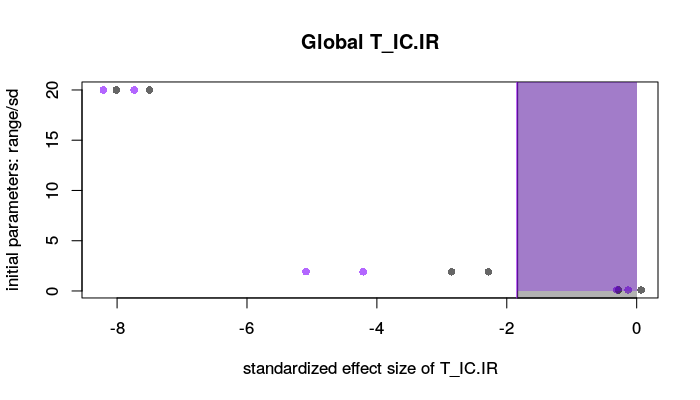
\includegraphics[width=\maxwidth]{figure/External_filter_Results_plots_initial_param1-1} 

}

\caption[Global $T_{IC/IR}$ SES and initial parameters values]{Global $T_{IC/IR}$ SES and initial parameters values: Standardized effect size of $T_{IC/IR}$ in function of the strength of external filter defined by the ratio of the inital range parameter by the initial standard error parameter. Colored area represent the mean confidence interval of SES values ($alpha = 0.95$). Trait a (normal) in black and b (uniform) in purple.\label{fig:External_filter_Results_plots_initial_param1}}
\end{figure}


\end{knitrout}

\begin{knitrout}\small
\definecolor{shadecolor}{rgb}{0.969, 0.969, 0.969}\color{fgcolor}\begin{kframe}
\begin{alltt}
\hlkwd{plot}\hlstd{(meanSES.3glob.norm_Tpcpr, init_param,} \hlkwc{pch} \hlstd{=} \hlnum{16}\hlstd{,} \hlkwc{col} \hlstd{=} \hlkwd{rgb}\hlstd{(}\hlnum{0}\hlstd{,} \hlnum{0}\hlstd{,} \hlnum{0}\hlstd{,} \hlnum{0.6}\hlstd{),}
     \hlkwc{main} \hlstd{=} \hlstr{"Global T_PC.PR"}\hlstd{,}
     \hlkwc{xlim} \hlstd{=} \hlkwd{c}\hlstd{(}\hlkwd{min}\hlstd{(}\hlkwd{c}\hlstd{(meanSES.3glob.norm_Tpcpr, meanSES.3glob.uni_Tpcpr),}
            \hlkwc{na.rm} \hlstd{= T),} \hlnum{0}\hlstd{),}
     \hlkwc{xlab} \hlstd{=} \hlstr{"standardized effect size of T_PC.PR"}\hlstd{,}
     \hlkwc{ylab} \hlstd{=} \hlstr{"initial parameters: range/sd"}\hlstd{)}
\hlkwd{points}\hlstd{(meanSES.3glob.uni_Tpcpr, init_param,} \hlkwc{pch} \hlstd{=} \hlnum{16}\hlstd{,} \hlkwc{col} \hlstd{=} \hlkwd{rgb}\hlstd{(}\hlnum{0.5}\hlstd{,} \hlnum{0}\hlstd{,} \hlnum{1}\hlstd{,} \hlnum{0.6}\hlstd{))}
\hlkwd{abline}\hlstd{(}\hlkwc{v} \hlstd{=} \hlkwd{mean}\hlstd{(meanSES.INF_glob.norm_Tpcpr,} \hlkwc{na.rm} \hlstd{= T))}
\hlkwd{abline}\hlstd{(}\hlkwc{v} \hlstd{=} \hlkwd{mean}\hlstd{(meanSES.INF_glob.uni_Tpcpr,} \hlkwc{na.rm} \hlstd{= T),} \hlkwc{col} \hlstd{=} \hlstr{"purple"}\hlstd{)}
\hlkwd{rect}\hlstd{(}\hlkwd{mean}\hlstd{(meanSES.INF_glob.norm_Tpcpr,} \hlkwc{na.rm} \hlstd{= T),} \hlopt{-}\hlnum{1}\hlstd{,} \hlnum{0}\hlstd{,} \hlkwd{max}\hlstd{(modeled_param_norm.loc)} \hlopt{+} \hlnum{1}\hlstd{,}
     \hlkwc{col} \hlstd{=} \hlkwd{rgb}\hlstd{(}\hlnum{0}\hlstd{,} \hlnum{0}\hlstd{,} \hlnum{0}\hlstd{,} \hlnum{0.3}\hlstd{),} \hlkwc{border} \hlstd{=} \hlnum{NA}\hlstd{)}
\hlkwd{rect}\hlstd{(}\hlkwd{mean}\hlstd{(meanSES.INF_glob.uni_Tpcpr,} \hlkwc{na.rm} \hlstd{= T),} \hlnum{0}\hlstd{,} \hlnum{0}\hlstd{,} \hlkwd{max}\hlstd{(modeled_param_uni.loc),}
     \hlkwc{col} \hlstd{=} \hlkwd{rgb}\hlstd{(}\hlnum{0.5}\hlstd{,} \hlnum{0}\hlstd{,} \hlnum{1}\hlstd{,} \hlnum{0.3}\hlstd{),} \hlkwc{border} \hlstd{=} \hlnum{NA}\hlstd{)}
\end{alltt}
\end{kframe}\begin{figure}

{\centering 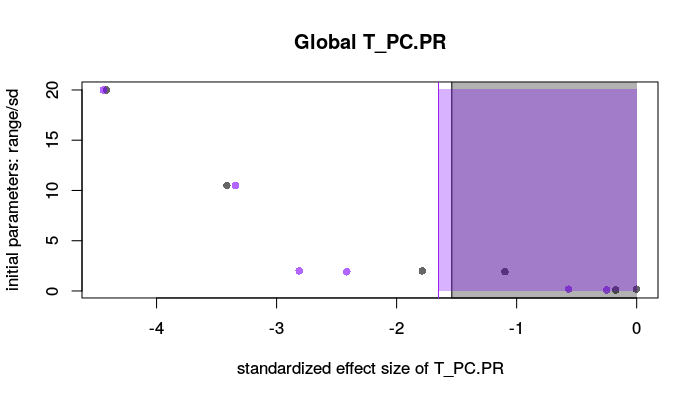
\includegraphics[width=\maxwidth]{figure/External_filter_Results_plots_initial_param2-1} 

}

\caption[Global $T_{PC/PR}$ SES and initial parameters values]{Global $T_{PC/PR}$ SES and initial parameters values: Standardized effect size of $T_{PC/PR}$ in function of the strength of external filter defined by the ratio of the inital range parameter by the initial standard error parameter. Colored area represent the mean confidence interval of SES values ($alpha = 0.95$). Trait a (normal) in black and b (uniform) in purple.\label{fig:External_filter_Results_plots_initial_param2}}
\end{figure}


\end{knitrout}
  
  \subsubsubsection {Global $T_{IC/IR}$ and $T_{PC/PR}$ SES values against modeled parameter values}
  
We can verify the consistency of our results by plotting SES values against the modeled parameters values (Fig. \ref{fig:External_filter_Results_plots_modeled_param1} and \ref{fig:External_filter_Results_plots_modeled_param2}). 

\begin{knitrout}\small
\definecolor{shadecolor}{rgb}{0.969, 0.969, 0.969}\color{fgcolor}\begin{kframe}
\begin{alltt}
\hlstd{mean_range_com.interm} \hlkwb{<-} \hlkwd{t}\hlstd{(}\hlkwd{matrix}\hlstd{(}\hlkwd{unlist}\hlstd{(}\hlkwd{lapply}\hlstd{(mean_range_com,} \hlkwa{function}\hlstd{(}\hlkwc{x}\hlstd{) x)),} \hlkwc{nrow} \hlstd{=} \hlnum{2}\hlstd{))}
\hlstd{mean_sd_of_com} \hlkwb{<-} \hlkwd{unlist}\hlstd{(}\hlkwd{lapply}\hlstd{(sd.com_stock3,} \hlkwa{function}\hlstd{(}\hlkwc{x}\hlstd{)} \hlkwd{mean}\hlstd{(x)))}

\hlstd{modeled_param_norm} \hlkwb{<-} \hlstd{mean_range_com.interm[,} \hlnum{1}\hlstd{]} \hlopt{/} \hlstd{mean_sd_of_com}
\hlstd{modeled_param_uni} \hlkwb{<-} \hlstd{mean_range_com.interm[,} \hlnum{2}\hlstd{]} \hlopt{/} \hlstd{mean_sd_of_com}

\hlkwd{plot}\hlstd{(meanSES.3glob.norm_Ticir, modeled_param_norm,} \hlkwc{pch} \hlstd{=} \hlnum{16}\hlstd{,}
  \hlkwc{main} \hlstd{=} \hlstr{"Global T_IC.IR"}\hlstd{,}
  \hlkwc{xlim} \hlstd{=} \hlkwd{c}\hlstd{(}\hlkwd{min}\hlstd{(}\hlkwd{c}\hlstd{(meanSES.3glob.norm_Ticir, meanSES.3glob.uni_Ticir),} \hlkwc{na.rm} \hlstd{= T),} \hlnum{0}\hlstd{),}
  \hlkwc{ylim} \hlstd{=} \hlkwd{c}\hlstd{(}\hlnum{0}\hlstd{,} \hlkwd{min}\hlstd{(}\hlkwd{max}\hlstd{(}\hlkwd{c}\hlstd{(modeled_param_norm, modeled_param_uni),} \hlkwc{na.rm} \hlstd{= T),} \hlnum{100}\hlstd{)),}
  \hlkwc{xlab} \hlstd{=} \hlstr{"standardized effect size of T_IC.IR"}\hlstd{,}
  \hlkwc{ylab} \hlstd{=} \hlstr{"modeled parameters: range/sd"}\hlstd{)}
\hlkwd{points}\hlstd{(meanSES.3glob.uni_Ticir, modeled_param_uni,} \hlkwc{pch} \hlstd{=} \hlnum{16}\hlstd{,} \hlkwc{col} \hlstd{=} \hlkwd{rgb}\hlstd{(}\hlnum{0.5}\hlstd{,} \hlnum{0}\hlstd{,} \hlnum{1}\hlstd{,} \hlnum{0.6}\hlstd{))}
\hlkwd{abline}\hlstd{(}\hlkwc{v} \hlstd{=} \hlkwd{mean}\hlstd{(meanSES.INF_glob.norm_Ticir,} \hlkwc{na.rm} \hlstd{= T))}
\hlkwd{abline}\hlstd{(}\hlkwc{v} \hlstd{=} \hlkwd{mean}\hlstd{(meanSES.INF_glob.uni_Ticir,} \hlkwc{na.rm} \hlstd{= T),} \hlkwc{col} \hlstd{=} \hlstr{"purple"}\hlstd{)}
\hlkwd{rect}\hlstd{(}\hlkwd{mean}\hlstd{(meanSES.INF_glob.norm_Ticir,} \hlkwc{na.rm} \hlstd{= T),} \hlopt{-}\hlnum{1}\hlstd{,} \hlnum{0}\hlstd{,} \hlkwd{max}\hlstd{(modeled_param_norm)} \hlopt{+} \hlnum{1}\hlstd{,}
  \hlkwc{col} \hlstd{=} \hlkwd{rgb}\hlstd{(}\hlnum{0}\hlstd{,} \hlnum{0}\hlstd{,} \hlnum{0}\hlstd{,} \hlnum{0.3}\hlstd{),} \hlkwc{border} \hlstd{=} \hlnum{NA}\hlstd{)}
\hlkwd{rect}\hlstd{(}\hlkwd{mean}\hlstd{(meanSES.INF_glob.uni_Ticir,} \hlkwc{na.rm} \hlstd{= T),} \hlnum{0}\hlstd{,} \hlnum{0}\hlstd{,} \hlkwd{max}\hlstd{(modeled_param_uni),}
  \hlkwc{col} \hlstd{=} \hlkwd{rgb}\hlstd{(}\hlnum{0.5}\hlstd{,} \hlnum{0}\hlstd{,} \hlnum{1}\hlstd{,} \hlnum{0.3}\hlstd{),} \hlkwc{border} \hlstd{=} \hlnum{NA}\hlstd{)}
\end{alltt}
\end{kframe}\begin{figure}

{\centering 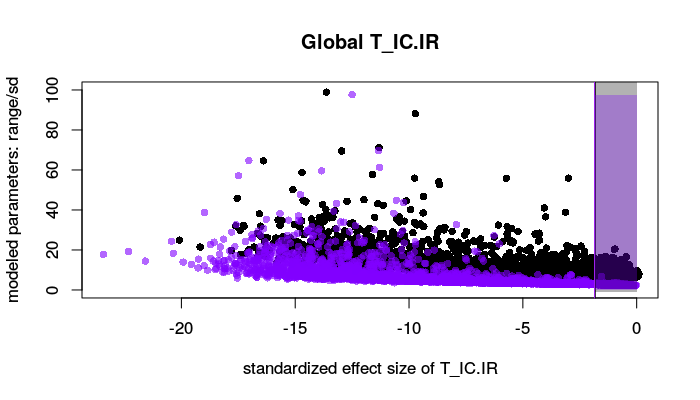
\includegraphics[width=\maxwidth]{figure/External_filter_Results_plots_modeled_param1-1} 

}

\caption[Global $T_{IC/IR}$ SES and modeled parameters values]{Global $T_{IC/IR}$ SES and modeled parameters values: Standardized effect size of $T_{IC/IR}$ in function of the strength of external filter defined by the ratio of the modeled range parameter by the modeled standard error parameter. Colored area represent the mean confidence interval of SES values ($alpha = 0.95$). Trait a (normal) in black and b (uniform) in purple.\label{fig:External_filter_Results_plots_modeled_param1}}
\end{figure}


\end{knitrout}

\begin{knitrout}\small
\definecolor{shadecolor}{rgb}{0.969, 0.969, 0.969}\color{fgcolor}\begin{kframe}
\begin{alltt}
\hlkwd{plot}\hlstd{(meanSES.3glob.norm_Tpcpr, modeled_param_norm,} \hlkwc{pch} \hlstd{=} \hlnum{16}\hlstd{,}
  \hlkwc{main} \hlstd{=} \hlstr{"Global T_PC.PR"}\hlstd{,}
  \hlkwc{xlim} \hlstd{=} \hlkwd{c}\hlstd{(}\hlkwd{min}\hlstd{(}\hlkwd{c}\hlstd{(meanSES.3glob.norm_Tpcpr, meanSES.3glob.uni_Tpcpr),}
    \hlkwc{na.rm} \hlstd{= T),} \hlnum{0}\hlstd{),}
  \hlkwc{ylim} \hlstd{=} \hlkwd{c}\hlstd{(}\hlnum{0}\hlstd{,} \hlkwd{min}\hlstd{(}\hlkwd{max}\hlstd{(}\hlkwd{c}\hlstd{(modeled_param_norm, modeled_param_uni),} \hlkwc{na.rm} \hlstd{= T),} \hlnum{100}\hlstd{)),}
  \hlkwc{xlab} \hlstd{=} \hlstr{"standardized effect size of T_PC.PR"}\hlstd{,}
  \hlkwc{ylab} \hlstd{=} \hlstr{"modeled parameters: range/sd"}\hlstd{)}
\hlkwd{points}\hlstd{(meanSES.3glob.uni_Tpcpr, modeled_param_uni,} \hlkwc{pch} \hlstd{=} \hlnum{16}\hlstd{,} \hlkwc{col} \hlstd{=} \hlkwd{rgb}\hlstd{(}\hlnum{0.5}\hlstd{,} \hlnum{0}\hlstd{,} \hlnum{1}\hlstd{,} \hlnum{0.6}\hlstd{))}
\hlkwd{abline}\hlstd{(}\hlkwc{v} \hlstd{=} \hlkwd{mean}\hlstd{(meanSES.INF_glob.norm_Tpcpr,} \hlkwc{na.rm} \hlstd{= T))}
\hlkwd{abline}\hlstd{(}\hlkwc{v} \hlstd{=} \hlkwd{mean}\hlstd{(meanSES.INF_glob.uni_Tpcpr,} \hlkwc{na.rm} \hlstd{= T),} \hlkwc{col} \hlstd{=} \hlstr{"purple"}\hlstd{)}
\hlkwd{rect}\hlstd{(}\hlkwd{mean}\hlstd{(meanSES.INF_glob.norm_Tpcpr,} \hlkwc{na.rm} \hlstd{= T),} \hlopt{-}\hlnum{1}\hlstd{,} \hlnum{0}\hlstd{,} \hlkwd{max}\hlstd{(modeled_param_norm)} \hlopt{+} \hlnum{1}\hlstd{,}
  \hlkwc{col} \hlstd{=} \hlkwd{rgb}\hlstd{(}\hlnum{0}\hlstd{,} \hlnum{0}\hlstd{,} \hlnum{0}\hlstd{,} \hlnum{0.3}\hlstd{),} \hlkwc{border} \hlstd{=} \hlnum{NA}\hlstd{)}
\hlkwd{rect}\hlstd{(}\hlkwd{mean}\hlstd{(meanSES.INF_glob.uni_Tpcpr,} \hlkwc{na.rm} \hlstd{= T),} \hlnum{0}\hlstd{,} \hlnum{0}\hlstd{,} \hlkwd{max}\hlstd{(modeled_param_uni),}
  \hlkwc{col} \hlstd{=} \hlkwd{rgb}\hlstd{(}\hlnum{0.5}\hlstd{,} \hlnum{0}\hlstd{,} \hlnum{1}\hlstd{,} \hlnum{0.3}\hlstd{),} \hlkwc{border} \hlstd{=} \hlnum{NA}\hlstd{)}
\end{alltt}
\end{kframe}\begin{figure}

{\centering 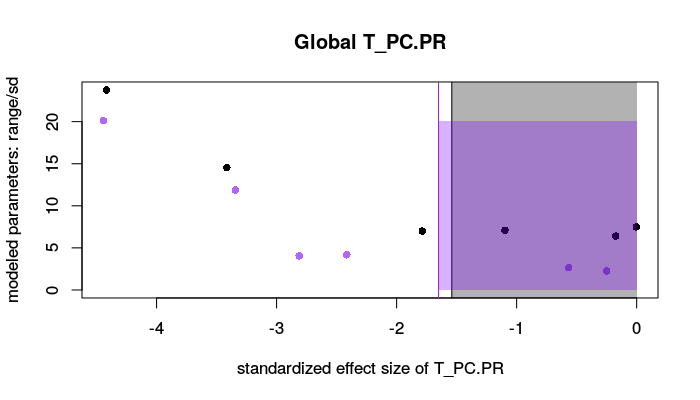
\includegraphics[width=\maxwidth]{figure/External_filter_Results_plots_modeled_param2-1} 

}

\caption[Global $T_{PC/PR}$ SES and modeled parameters values]{Global $T_{PC/PR}$ SES and modeled parameters values: Standardized effect size of $T_{PC/PR}$ in function of the strength of external filter defined by the ratio of the modeled range parameter by the modeled standard error parameter. Colored area represent the mean confidence interval of SES values ($alpha = 0.95$). Trait a (normal) in black and b (uniform) in purple.\label{fig:External_filter_Results_plots_modeled_param2}}
\end{figure}


\end{knitrout}


  \subsection {Conclusion on the power of $T_{IC/IR}$ to detect external filtering}

To conclude on the power of $T_{IC/IR}$ to detect external filtering, we compute exponential linear model and identify the strength from which the beta-error is inferior to 0.05. This strength is define by the two ratio of the initial parameters \texttt{param\_range} and \texttt{sd\_mean.param}. 

\begin{knitrout}\small
\definecolor{shadecolor}{rgb}{0.969, 0.969, 0.969}\color{fgcolor}\begin{kframe}
\begin{alltt}
\hlkwd{plot}\hlstd{(meanSES.3loc.norm_Ticir} \hlopt{~} \hlstd{init_param.loc,} \hlkwc{col} \hlstd{=} \hlkwd{rgb}\hlstd{(}\hlnum{0}\hlstd{,} \hlnum{0}\hlstd{,} \hlnum{0}\hlstd{,} \hlnum{0.2}\hlstd{),}
     \hlkwc{ylim} \hlstd{=} \hlkwd{c}\hlstd{(}\hlkwd{min}\hlstd{(}\hlkwd{c}\hlstd{(meanSES.3loc.norm_Ticir , meanSES.3loc.uni_Ticir,}
                  \hlstd{meanSES.3glob.norm_Ticir, meanSES.3glob.uni_Ticir),} \hlkwc{na.rm} \hlstd{= T),} \hlnum{0}\hlstd{),}
     \hlkwc{main} \hlstd{=} \hlstr{"Global T_IC.IR"}\hlstd{,}
     \hlkwc{ylab} \hlstd{=} \hlstr{"standardized effect size of T_IC.IR"}\hlstd{,}
     \hlkwc{xlab} \hlstd{=} \hlstr{"initial parameters: range/sd"}\hlstd{,}
     \hlkwc{type} \hlstd{=} \hlstr{"n"}\hlstd{)}
\hlcom{#points(meanSES.3loc.uni_Ticir ~ init_param.loc, col = rgb(0.5, 0, 1, 0.2))}

\hlkwd{points}\hlstd{(meanSES.3glob.norm_Ticir} \hlopt{~} \hlstd{init_param,} \hlkwc{pch} \hlstd{=} \hlnum{16}\hlstd{,} \hlkwc{col} \hlstd{=} \hlkwd{rgb}\hlstd{(}\hlnum{0}\hlstd{,} \hlnum{0}\hlstd{,} \hlnum{0}\hlstd{,} \hlnum{0.5}\hlstd{),} \hlkwc{cex} \hlstd{=} \hlnum{1.2}\hlstd{)}
\hlstd{lm.norm} \hlkwb{<-} \hlkwd{lm}\hlstd{(meanSES.3glob.norm_Ticir} \hlopt{~} \hlkwd{log}\hlstd{(init_param))}
\hlstd{lm.norm_conf} \hlkwb{<-} \hlkwd{confint}\hlstd{(lm.norm,} \hlkwc{level} \hlstd{=} \hlnum{0.90}\hlstd{)}
\hlkwd{curve}\hlstd{(lm.norm}\hlopt{$}\hlstd{coef[}\hlnum{1}\hlstd{]} \hlopt{+} \hlkwd{log}\hlstd{(x)} \hlopt{*} \hlstd{(lm.norm}\hlopt{$}\hlstd{coef[}\hlnum{2}\hlstd{]),} \hlkwc{add} \hlstd{= T,} \hlkwc{lwd} \hlstd{=} \hlnum{3}\hlstd{,} \hlkwc{col} \hlstd{=} \hlkwd{rgb}\hlstd{(}\hlnum{0}\hlstd{,} \hlnum{0}\hlstd{,} \hlnum{0}\hlstd{,} \hlnum{1}\hlstd{))}
\hlkwd{curve}\hlstd{(lm.norm_conf [}\hlnum{1}\hlstd{,} \hlnum{1}\hlstd{]} \hlopt{+} \hlkwd{log}\hlstd{(x)} \hlopt{*} \hlstd{lm.norm_conf [}\hlnum{2}\hlstd{,} \hlnum{1}\hlstd{],} \hlkwc{add} \hlstd{= T,} \hlkwc{lty} \hlstd{=} \hlnum{2}\hlstd{,} \hlkwc{col} \hlstd{=} \hlkwd{rgb}\hlstd{(}\hlnum{0}\hlstd{,} \hlnum{0}\hlstd{,} \hlnum{0}\hlstd{,} \hlnum{1}\hlstd{))}
\hlkwd{curve}\hlstd{(lm.norm_conf [}\hlnum{1}\hlstd{,} \hlnum{2}\hlstd{]} \hlopt{+} \hlkwd{log}\hlstd{(x)} \hlopt{*} \hlstd{lm.norm_conf [}\hlnum{2}\hlstd{,} \hlnum{2}\hlstd{],} \hlkwc{add} \hlstd{= T,} \hlkwc{lty} \hlstd{=} \hlnum{2}\hlstd{,} \hlkwc{col} \hlstd{=} \hlkwd{rgb}\hlstd{(}\hlnum{0}\hlstd{,} \hlnum{0}\hlstd{,} \hlnum{0}\hlstd{,} \hlnum{1}\hlstd{))}

\hlkwd{points}\hlstd{(meanSES.3glob.uni_Ticir} \hlopt{~} \hlstd{init_param,} \hlkwc{pch} \hlstd{=} \hlnum{16}\hlstd{,} \hlkwc{col} \hlstd{=} \hlkwd{rgb}\hlstd{(}\hlnum{0.5}\hlstd{,} \hlnum{0}\hlstd{,} \hlnum{1}\hlstd{,} \hlnum{0.5}\hlstd{),} \hlkwc{cex} \hlstd{=} \hlnum{1.2}\hlstd{)}
\hlstd{lm.uni} \hlkwb{<-} \hlkwd{lm}\hlstd{(meanSES.3glob.uni_Ticir} \hlopt{~} \hlkwd{log}\hlstd{(init_param))}
\hlstd{lm.uni_conf} \hlkwb{<-} \hlkwd{confint}\hlstd{(lm.uni,} \hlkwc{level} \hlstd{=} \hlnum{0.90}\hlstd{)}
\hlkwd{curve}\hlstd{(lm.uni}\hlopt{$}\hlstd{coef[}\hlnum{1}\hlstd{]} \hlopt{+} \hlkwd{log}\hlstd{(x)} \hlopt{*} \hlstd{(lm.uni}\hlopt{$}\hlstd{coef[}\hlnum{2}\hlstd{]),} \hlkwc{add} \hlstd{= T,} \hlkwc{lwd} \hlstd{=} \hlnum{3}\hlstd{,}  \hlkwc{col} \hlstd{=} \hlkwd{rgb}\hlstd{(}\hlnum{0.5}\hlstd{,} \hlnum{0}\hlstd{,} \hlnum{1}\hlstd{,} \hlnum{1}\hlstd{))}
\hlkwd{curve}\hlstd{(lm.uni_conf [}\hlnum{1}\hlstd{,} \hlnum{1}\hlstd{]} \hlopt{+} \hlkwd{log}\hlstd{(x)} \hlopt{*} \hlstd{lm.uni_conf [}\hlnum{2}\hlstd{,} \hlnum{1}\hlstd{],} \hlkwc{add} \hlstd{= T,} \hlkwc{lty} \hlstd{=} \hlnum{2}\hlstd{,} \hlkwc{col} \hlstd{=} \hlkwd{rgb}\hlstd{(}\hlnum{0.5}\hlstd{,} \hlnum{0}\hlstd{,} \hlnum{1}\hlstd{,} \hlnum{1}\hlstd{))}
\hlkwd{curve}\hlstd{(lm.uni_conf [}\hlnum{1}\hlstd{,} \hlnum{2}\hlstd{]} \hlopt{+} \hlkwd{log}\hlstd{(x)} \hlopt{*} \hlstd{lm.uni_conf [}\hlnum{2}\hlstd{,} \hlnum{2}\hlstd{],} \hlkwc{add} \hlstd{= T,} \hlkwc{lty} \hlstd{=} \hlnum{2}\hlstd{,} \hlkwc{col} \hlstd{=} \hlkwd{rgb}\hlstd{(}\hlnum{0.5}\hlstd{,} \hlnum{0}\hlstd{,} \hlnum{1}\hlstd{,} \hlnum{1}\hlstd{))}


\hlkwd{rect}\hlstd{(}\hlopt{-}\hlnum{1}\hlstd{,} \hlkwd{mean}\hlstd{(}\hlkwd{c}\hlstd{(SES.inf.MEAN.uni_Ticir, meanSES.INF_glob.uni_Ticir),} \hlkwc{na.rm} \hlstd{= T),} \hlkwd{max}\hlstd{(init_param),} \hlnum{10}\hlstd{,}
  \hlkwc{col} \hlstd{=} \hlkwd{rgb}\hlstd{(}\hlnum{0.5}\hlstd{,} \hlnum{0}\hlstd{,} \hlnum{1}\hlstd{,} \hlnum{0.3}\hlstd{),} \hlkwc{border} \hlstd{=} \hlnum{NA}\hlstd{)}

\hlkwd{rect}\hlstd{(}\hlopt{-}\hlnum{1}\hlstd{,} \hlkwd{mean}\hlstd{(}\hlkwd{c}\hlstd{(SES.inf.MEAN.norm_Ticir, meanSES.INF_glob.norm_Ticir),} \hlkwc{na.rm} \hlstd{= T),} \hlkwd{max}\hlstd{(init_param)} \hlopt{+} \hlnum{10}\hlstd{,} \hlnum{10}\hlstd{,}
  \hlkwc{col} \hlstd{=} \hlkwd{rgb}\hlstd{(}\hlnum{0}\hlstd{,} \hlnum{0}\hlstd{,} \hlnum{0}\hlstd{,} \hlnum{0.3}\hlstd{),} \hlkwc{border} \hlstd{=} \hlnum{NA}\hlstd{)}
\end{alltt}
\end{kframe}\begin{figure}

{\centering 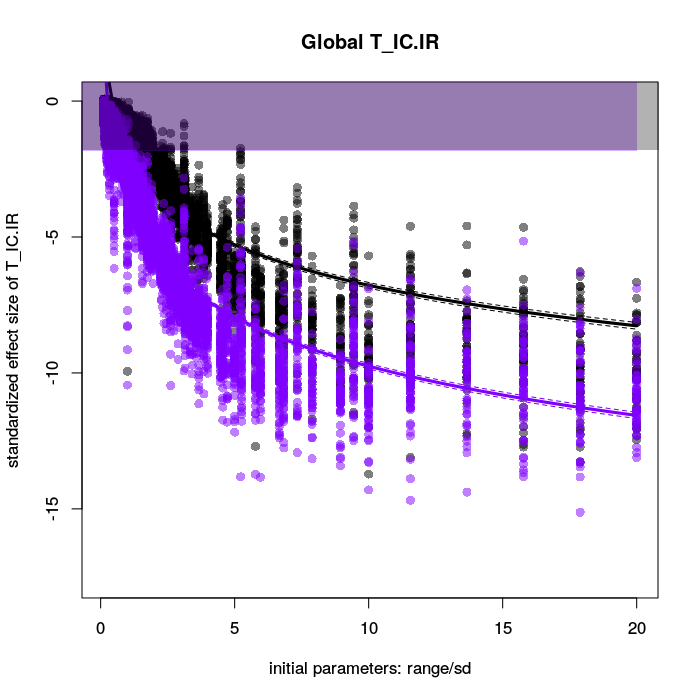
\includegraphics[width=\maxwidth]{figure/Ex_conc_plot1-1} 

}

\caption[Power of $T_{IC/IR}$ to detect external filtering]{Power of $T_{IC/IR}$ to detect external filtering: Standardised Effect Size (SES) of $T_{IC/IR}$ in relation to the strength of external filtering. Trait 'a' normally distributed is shown in black, traits 'b' uniformally distributed in purple. Close circles represent global SES values. The exponential linear model is presented with 5 percents confidence interval on both side. Colored area represent the mean confidence interval of SES values ($alpha = 0.95$)\label{fig:Ex_conc_plot1}}
\end{figure}


\end{knitrout}

\begin{knitrout}\small
\definecolor{shadecolor}{rgb}{0.969, 0.969, 0.969}\color{fgcolor}\begin{kframe}
\begin{alltt}
\hlstd{yy.norm} \hlkwb{<-} \hlkwd{mean}\hlstd{(}\hlkwd{c}\hlstd{(SES.inf.MEAN.norm_Ticir, meanSES.INF_glob.norm_Ticir),} \hlkwc{na.rm} \hlstd{= T)}
\hlstd{yy.uni} \hlkwb{<-} \hlkwd{mean}\hlstd{(}\hlkwd{c}\hlstd{(SES.inf.MEAN.uni_Ticir, meanSES.INF_glob.uni_Ticir),} \hlkwc{na.rm} \hlstd{= T)}

\hlstd{param_beta0.05_Ticir.norm} \hlkwb{<-} \hlkwd{exp}\hlstd{( (yy.norm} \hlopt{-} \hlstd{lm.norm_conf [}\hlnum{1}\hlstd{,} \hlnum{2}\hlstd{])} \hlopt{/} \hlstd{lm.norm_conf [}\hlnum{2}\hlstd{,} \hlnum{2}\hlstd{] )}
\hlstd{param_beta0.05_Ticir.uni} \hlkwb{<-} \hlkwd{exp}\hlstd{( (yy.uni} \hlopt{-} \hlstd{lm.uni_conf [}\hlnum{1}\hlstd{,} \hlnum{2}\hlstd{])} \hlopt{/} \hlstd{lm.uni_conf [}\hlnum{2}\hlstd{,} \hlnum{2}\hlstd{] )}
\end{alltt}
\end{kframe}
\end{knitrout}


For the trait "a" normally distributed, the power of $T_{IC/IR}$ is satisfying if the ratio of the initial parameter is superior to
 1.07. For the trait "b" uniformally distributed, this value is 0.51. 
 Further investigation on real data with different strength of external filtering are needed to complete these simulated values.

 




  \subsection {Conclusion on the power of $T_{PC/PR}$ to detect external filtering}

To conclude on the power of $T_{PC/PR}$ to detect external filtering, we compute exponential linear model and identify the strength from which the beta-error is inferior to 0.05. This strength is define by the two ratio of the initial parameters \texttt{param\_range} and \texttt{sd\_mean.param}. 

\begin{knitrout}\small
\definecolor{shadecolor}{rgb}{0.969, 0.969, 0.969}\color{fgcolor}\begin{kframe}
\begin{alltt}
\hlkwd{plot}\hlstd{(meanSES.3loc.norm_Tpcpr} \hlopt{~} \hlstd{init_param.loc,} \hlkwc{col} \hlstd{=} \hlkwd{rgb}\hlstd{(}\hlnum{0}\hlstd{,} \hlnum{0}\hlstd{,} \hlnum{0}\hlstd{,} \hlnum{0.2}\hlstd{),}
     \hlkwc{ylim} \hlstd{=} \hlkwd{c}\hlstd{(}\hlkwd{min}\hlstd{(}\hlkwd{c}\hlstd{(meanSES.3loc.norm_Tpcpr , meanSES.3loc.uni_Tpcpr,}
                  \hlstd{meanSES.3glob.norm_Tpcpr, meanSES.3glob.uni_Tpcpr),} \hlkwc{na.rm} \hlstd{= T),} \hlnum{0}\hlstd{),}
     \hlkwc{main} \hlstd{=} \hlstr{"Global T_PC.IR"}\hlstd{,}
     \hlkwc{ylab} \hlstd{=} \hlstr{"standardized effect size of T_PC.IR"}\hlstd{,}
     \hlkwc{xlab} \hlstd{=} \hlstr{"initial parameters: range/sd"}\hlstd{,}
     \hlkwc{type} \hlstd{=} \hlstr{"n"}\hlstd{)}
\hlcom{#points(meanSES.3loc.uni_Tpcpr ~ init_param.loc, col = rgb(0.5, 0, 1, 0.2))}

\hlkwd{points}\hlstd{(meanSES.3glob.norm_Tpcpr} \hlopt{~} \hlstd{init_param,} \hlkwc{pch} \hlstd{=} \hlnum{16}\hlstd{,} \hlkwc{col} \hlstd{=} \hlkwd{rgb}\hlstd{(}\hlnum{0}\hlstd{,} \hlnum{0}\hlstd{,} \hlnum{0}\hlstd{,} \hlnum{0.5}\hlstd{),} \hlkwc{cex} \hlstd{=} \hlnum{1.2}\hlstd{)}
\hlstd{lm.norm} \hlkwb{<-} \hlkwd{lm}\hlstd{(meanSES.3glob.norm_Tpcpr} \hlopt{~} \hlkwd{log}\hlstd{(init_param))}
\hlstd{lm.norm_conf} \hlkwb{<-} \hlkwd{confint}\hlstd{(lm.norm,} \hlkwc{level} \hlstd{=} \hlnum{0.90}\hlstd{)}
\hlkwd{curve}\hlstd{(lm.norm}\hlopt{$}\hlstd{coef[}\hlnum{1}\hlstd{]} \hlopt{+} \hlkwd{log}\hlstd{(x)} \hlopt{*} \hlstd{(lm.norm}\hlopt{$}\hlstd{coef[}\hlnum{2}\hlstd{]),} \hlkwc{add} \hlstd{= T,} \hlkwc{lwd} \hlstd{=} \hlnum{3}\hlstd{,} \hlkwc{col} \hlstd{=} \hlkwd{rgb}\hlstd{(}\hlnum{0}\hlstd{,} \hlnum{0}\hlstd{,} \hlnum{0}\hlstd{,} \hlnum{1}\hlstd{))}
\hlkwd{curve}\hlstd{(lm.norm_conf [}\hlnum{1}\hlstd{,} \hlnum{1}\hlstd{]} \hlopt{+} \hlkwd{log}\hlstd{(x)} \hlopt{*} \hlstd{lm.norm_conf [}\hlnum{2}\hlstd{,} \hlnum{1}\hlstd{],} \hlkwc{add} \hlstd{= T,} \hlkwc{lty} \hlstd{=} \hlnum{2}\hlstd{,} \hlkwc{col} \hlstd{=} \hlkwd{rgb}\hlstd{(}\hlnum{0}\hlstd{,} \hlnum{0}\hlstd{,} \hlnum{0}\hlstd{,} \hlnum{1}\hlstd{))}
\hlkwd{curve}\hlstd{(lm.norm_conf [}\hlnum{1}\hlstd{,} \hlnum{2}\hlstd{]} \hlopt{+} \hlkwd{log}\hlstd{(x)} \hlopt{*} \hlstd{lm.norm_conf [}\hlnum{2}\hlstd{,} \hlnum{2}\hlstd{],} \hlkwc{add} \hlstd{= T,} \hlkwc{lty} \hlstd{=} \hlnum{2}\hlstd{,} \hlkwc{col} \hlstd{=} \hlkwd{rgb}\hlstd{(}\hlnum{0}\hlstd{,} \hlnum{0}\hlstd{,} \hlnum{0}\hlstd{,} \hlnum{1}\hlstd{))}

\hlkwd{points}\hlstd{(meanSES.3glob.uni_Tpcpr} \hlopt{~} \hlstd{init_param,} \hlkwc{pch} \hlstd{=} \hlnum{16}\hlstd{,} \hlkwc{col} \hlstd{=} \hlkwd{rgb}\hlstd{(}\hlnum{0.5}\hlstd{,} \hlnum{0}\hlstd{,} \hlnum{1}\hlstd{,} \hlnum{0.5}\hlstd{),} \hlkwc{cex} \hlstd{=} \hlnum{1.2}\hlstd{)}
\hlstd{lm.uni} \hlkwb{<-} \hlkwd{lm}\hlstd{(meanSES.3glob.uni_Tpcpr} \hlopt{~} \hlkwd{log}\hlstd{(init_param))}
\hlstd{lm.uni_conf} \hlkwb{<-} \hlkwd{confint}\hlstd{(lm.uni,} \hlkwc{level} \hlstd{=} \hlnum{0.90}\hlstd{)}
\hlkwd{curve}\hlstd{(lm.uni}\hlopt{$}\hlstd{coef[}\hlnum{1}\hlstd{]} \hlopt{+} \hlkwd{log}\hlstd{(x)} \hlopt{*} \hlstd{(lm.uni}\hlopt{$}\hlstd{coef[}\hlnum{2}\hlstd{]),} \hlkwc{add} \hlstd{= T,} \hlkwc{lwd} \hlstd{=} \hlnum{3}\hlstd{,}  \hlkwc{col} \hlstd{=} \hlkwd{rgb}\hlstd{(}\hlnum{0.5}\hlstd{,} \hlnum{0}\hlstd{,} \hlnum{1}\hlstd{,} \hlnum{1}\hlstd{))}
\hlkwd{curve}\hlstd{(lm.uni_conf [}\hlnum{1}\hlstd{,} \hlnum{1}\hlstd{]} \hlopt{+} \hlkwd{log}\hlstd{(x)} \hlopt{*} \hlstd{lm.uni_conf [}\hlnum{2}\hlstd{,} \hlnum{1}\hlstd{],} \hlkwc{add} \hlstd{= T,} \hlkwc{lty} \hlstd{=} \hlnum{2}\hlstd{,} \hlkwc{col} \hlstd{=} \hlkwd{rgb}\hlstd{(}\hlnum{0.5}\hlstd{,} \hlnum{0}\hlstd{,} \hlnum{1}\hlstd{,} \hlnum{1}\hlstd{))}
\hlkwd{curve}\hlstd{(lm.uni_conf [}\hlnum{1}\hlstd{,} \hlnum{2}\hlstd{]} \hlopt{+} \hlkwd{log}\hlstd{(x)} \hlopt{*} \hlstd{lm.uni_conf [}\hlnum{2}\hlstd{,} \hlnum{2}\hlstd{],} \hlkwc{add} \hlstd{= T,} \hlkwc{lty} \hlstd{=} \hlnum{2}\hlstd{,} \hlkwc{col} \hlstd{=} \hlkwd{rgb}\hlstd{(}\hlnum{0.5}\hlstd{,} \hlnum{0}\hlstd{,} \hlnum{1}\hlstd{,} \hlnum{1}\hlstd{))}


\hlkwd{rect}\hlstd{(}\hlopt{-}\hlnum{1}\hlstd{,} \hlkwd{mean}\hlstd{(}\hlkwd{c}\hlstd{(SES.inf.MEAN.uni_Tpcpr, meanSES.INF_glob.uni_Tpcpr),} \hlkwc{na.rm} \hlstd{= T),} \hlkwd{max}\hlstd{(init_param),} \hlnum{10}\hlstd{,}
  \hlkwc{col} \hlstd{=} \hlkwd{rgb}\hlstd{(}\hlnum{0.5}\hlstd{,} \hlnum{0}\hlstd{,} \hlnum{1}\hlstd{,} \hlnum{0.3}\hlstd{),} \hlkwc{border} \hlstd{=} \hlnum{NA}\hlstd{)}

\hlkwd{rect}\hlstd{(}\hlopt{-}\hlnum{1}\hlstd{,} \hlkwd{mean}\hlstd{(}\hlkwd{c}\hlstd{(SES.inf.MEAN.norm_Tpcpr, meanSES.INF_glob.norm_Tpcpr),} \hlkwc{na.rm} \hlstd{= T),} \hlkwd{max}\hlstd{(init_param)} \hlopt{+} \hlnum{10}\hlstd{,} \hlnum{10}\hlstd{,}
  \hlkwc{col} \hlstd{=} \hlkwd{rgb}\hlstd{(}\hlnum{0}\hlstd{,} \hlnum{0}\hlstd{,} \hlnum{0}\hlstd{,} \hlnum{0.3}\hlstd{),} \hlkwc{border} \hlstd{=} \hlnum{NA}\hlstd{)}
\end{alltt}
\end{kframe}\begin{figure}

{\centering 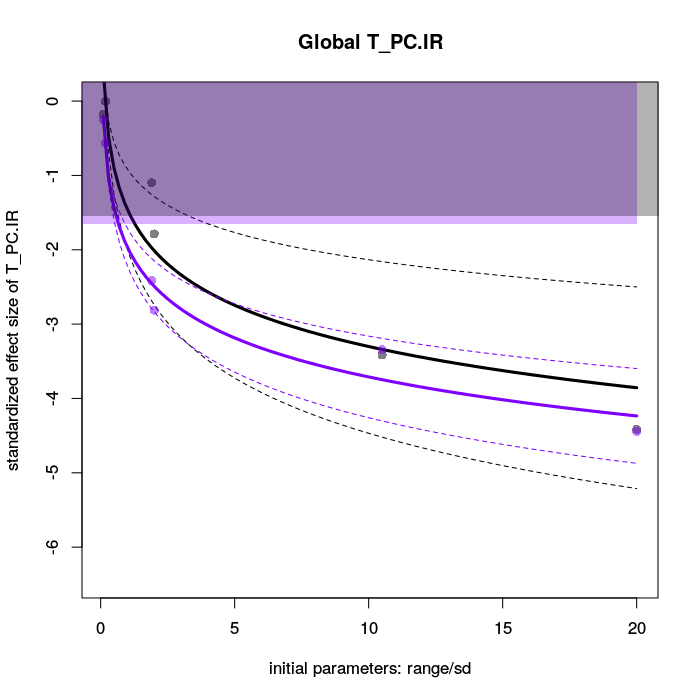
\includegraphics[width=\maxwidth]{figure/Ex_conc_plot2-1} 

}

\caption[Power of $T_{PC/PR}$ to detect external filtering]{Power of $T_{PC/PR}$ to detect external filtering: Standardised Effect Size (SES) of $T_{PC/PR}$ in relation to the strength of external filtering. Trait 'a' normally distributed is shown in black, traits 'b' uniformally distributed in purple. Close circles represent global SES values. The exponential linear model is represented with 5 percents confidence interval on both side. Colored area represent the mean confidence interval of SES values ($alpha = 0.95$)\label{fig:Ex_conc_plot2}}
\end{figure}


\end{knitrout}

\begin{knitrout}\small
\definecolor{shadecolor}{rgb}{0.969, 0.969, 0.969}\color{fgcolor}\begin{kframe}
\begin{alltt}
\hlstd{yy.norm} \hlkwb{<-} \hlkwd{mean}\hlstd{(}\hlkwd{c}\hlstd{(SES.inf.MEAN.norm_Tpcpr, meanSES.INF_glob.norm_Tpcpr),} \hlkwc{na.rm} \hlstd{= T)}
\hlstd{yy.uni} \hlkwb{<-} \hlkwd{mean}\hlstd{(}\hlkwd{c}\hlstd{(SES.inf.MEAN.uni_Tpcpr, meanSES.INF_glob.uni_Tpcpr),} \hlkwc{na.rm} \hlstd{= T)}

\hlstd{param_beta0.05_Tpcpr.norm} \hlkwb{<-} \hlkwd{exp}\hlstd{( (yy.norm} \hlopt{-} \hlstd{lm.norm_conf [}\hlnum{1}\hlstd{,} \hlnum{2}\hlstd{])} \hlopt{/} \hlstd{lm.norm_conf [}\hlnum{2}\hlstd{,} \hlnum{2}\hlstd{] )}
\hlstd{param_beta0.05_Tpcpr.uni} \hlkwb{<-} \hlkwd{exp}\hlstd{( (yy.uni} \hlopt{-} \hlstd{lm.uni_conf [}\hlnum{1}\hlstd{,} \hlnum{2}\hlstd{])} \hlopt{/} \hlstd{lm.uni_conf [}\hlnum{2}\hlstd{,} \hlnum{2}\hlstd{] )}
\end{alltt}
\end{kframe}
\end{knitrout}


For the trait "a" normally distributed, the power of $T_{PC/PR}$ is satisfying if the ratio of the initial parameter is superior to
 1.62. For the trait "b" uniformally distributed, this value is 0.78. 
 Further investigation on real data with different strength of external filtering are needed to complete these simulated values. As expected, $T_{PC/PR}$ is far less powerfull than $T_{IC/IR}$ to detect external filtering either with traits "a" (1.62 \textit{vs} 1.07) and "b" (0.78 \textit{vs} 0.51). This is due to the loss of information in $T_{PC/PR}$ when we compute the mean by population and exclude intra-populationnal variation from the test of external filter. 




































\cleardoublepage

\section{Internal and external filtering}

  \subsection{Randomization outline}
We use the same two parameters as for internal and external filtering analysis. The internal filtering is compute as in the section dedicated to internal filter. To add the effect of external filtering, we add a value to each individual belonging to a community, this values differing among communities.

\begin{knitrout}\small
\definecolor{shadecolor}{rgb}{0.969, 0.969, 0.969}\color{fgcolor}\begin{kframe}
\begin{alltt}
\hlcom{# Parameter for the distance between species mean trait values}
\hlstd{param_DIST_between_MEAN.init} \hlkwb{<-} \hlkwd{round}\hlstd{(}\hlkwd{sort}\hlstd{(}\hlkwd{seq}\hlstd{(}\hlnum{10}\hlstd{,} \hlnum{200}\hlstd{,} \hlkwc{length.out} \hlstd{= nb_param_val)),} \hlnum{2}\hlstd{)}
\hlstd{param_DIST_between_MEAN} \hlkwb{<-} \hlkwd{rep}\hlstd{(param_DIST_between_MEAN.init, N_repet_Param)}
\hlstd{mean_sd.param} \hlkwb{<-} \hlkwd{rep}\hlstd{(}\hlnum{10}\hlstd{, nperm)}

\hlcom{# Parameter for the variance in species mean trait values}
\hlstd{param_SD} \hlkwb{<-} \hlkwd{seq}\hlstd{(}\hlnum{10}\hlstd{,} \hlnum{100}\hlstd{,}\hlkwc{length.out} \hlstd{= nb_param_val)}
\hlstd{sd_mean.param} \hlkwb{<-} \hlkwd{sample} \hlstd{(}\hlkwd{rep}\hlstd{(param_SD, N_repet_Param),}
       \hlkwc{size} \hlstd{=} \hlkwd{length}\hlstd{(}\hlkwd{rep}\hlstd{(param_SD, N_repet_Param)),} \hlkwc{replace} \hlstd{= F)}
\hlstd{sd_sd.param} \hlkwb{<-} \hlkwd{rep}\hlstd{(}\hlnum{10}\hlstd{, nperm)}

\hlstd{nperm} \hlkwb{<-} \hlstd{N_repet_Param}\hlopt{*}\hlkwd{length}\hlstd{(param_SD)}
\end{alltt}
\end{kframe}
\end{knitrout}

\begin{knitrout}\small
\definecolor{shadecolor}{rgb}{0.969, 0.969, 0.969}\color{fgcolor}\begin{kframe}
\begin{alltt}
\hlcom{#Start simulation }
\hlstd{mean.sp_stock4} \hlkwb{<-} \hlkwd{list}\hlstd{()}
\hlstd{sd.sp_stock4} \hlkwb{<-} \hlkwd{list}\hlstd{()}
\hlstd{mean.com_stock4} \hlkwb{<-} \hlkwd{list}\hlstd{()}
\hlstd{sd.com_stock4} \hlkwb{<-} \hlkwd{list}\hlstd{()}
\hlstd{res.simu4} \hlkwb{<-} \hlkwd{list}\hlstd{()}
\hlstd{res.simu4.pval} \hlkwb{<-} \hlkwd{list}\hlstd{()}
\hlstd{res.simu.traits4} \hlkwb{<-} \hlkwd{list}\hlstd{()}

\hlkwa{for}\hlstd{(n} \hlkwa{in} \hlnum{1}\hlopt{:}\hlstd{nperm)\{}\hlcom{#for each permutation}

\hlstd{ex.sp4} \hlkwb{<-} \hlkwd{c}\hlstd{()}
\hlstd{ex.com4} \hlkwb{<-} \hlkwd{matrix}\hlstd{(}\hlnum{0}\hlstd{,} \hlkwc{nrow} \hlstd{=} \hlnum{10}\hlstd{,} \hlkwc{ncol} \hlstd{=} \hlnum{20}\hlstd{)}
\hlkwa{for}\hlstd{(i} \hlkwa{in} \hlnum{1}\hlopt{:} \hlnum{10}\hlstd{)\{}
 \hlstd{ex.com.interm} \hlkwb{<-} \hlkwd{table}\hlstd{(}\hlkwd{sample}\hlstd{(sp,} \hlkwc{size} \hlstd{=} \hlnum{100}\hlstd{,} \hlkwc{prob} \hlstd{=} \hlkwd{rlnorm}\hlstd{(}\hlnum{20}\hlstd{,} \hlnum{0}\hlstd{, sdlog),} \hlkwc{replace} \hlstd{= T))}
 \hlstd{ex.com4[i, sp}\hlopt \hlkwd{names}\hlstd{(ex.com.interm)]} \hlkwb{<-} \hlstd{ex.com.interm}
 \hlstd{ex.sp4} \hlkwb{<-} \hlkwd{c}\hlstd{(ex.sp4,} \hlkwd{rep}\hlstd{(sp,} \hlkwc{times} \hlstd{= ex.com4[i,]))}
\hlstd{\}}

\hlstd{ex.indplot4} \hlkwb{<-} \hlkwd{as.factor}\hlstd{(}\hlkwd{rep}\hlstd{(com,} \hlnum{100}\hlstd{))}


\hlcom{#Defining traits mean and sd by species }
\hlstd{mean_mean.param.interm} \hlkwb{<-} \hlkwd{seq}\hlstd{(max.value_traits} \hlopt{-} \hlstd{param_DIST_between_MEAN[n],}
        \hlstd{max.value_traits,} \hlkwc{length.out} \hlstd{=}
        \hlkwd{length}\hlstd{(}\hlkwd{unique}\hlstd{(param_DIST_between_MEAN)))}

\hlstd{mean_mean.param} \hlkwb{<-} \hlkwd{rep}\hlstd{(}\hlkwd{round}\hlstd{(}\hlkwd{sort}\hlstd{(mean_mean.param.interm),} \hlnum{2}\hlstd{),}
        \hlstd{N_repet_Param)}

\hlstd{mean.sp} \hlkwb{<-} \hlkwd{rnorm}\hlstd{(}\hlkwd{length}\hlstd{(}\hlkwd{unique}\hlstd{(sp)),} \hlkwc{mean} \hlstd{= mean_mean.param,} \hlkwc{sd} \hlstd{= mean_sd.param[n])}
\hlstd{sd.sp} \hlkwb{<-} \hlkwd{rnorm}\hlstd{(}\hlkwd{length}\hlstd{(}\hlkwd{unique}\hlstd{(sp)),} \hlkwc{mean} \hlstd{= sd_mean.param[n],} \hlkwc{sd} \hlstd{= sd_sd.param[n])}

\hlstd{ex.traits4} \hlkwb{<-} \hlkwd{array}\hlstd{(}\hlnum{NA}\hlstd{,} \hlkwc{dim} \hlstd{=} \hlkwd{c}\hlstd{(}\hlnum{1000}\hlstd{,} \hlnum{2}\hlstd{))}
\hlkwd{colnames}\hlstd{(ex.traits4)} \hlkwb{<-} \hlkwd{paste}\hlstd{(}\hlstr{"trait"}\hlstd{,} \hlkwd{c}\hlstd{(}\hlstr{"a"}\hlstd{,} \hlstr{"b"}\hlstd{),} \hlkwc{sep} \hlstd{=} \hlstr{" "}\hlstd{)}

\hlkwa{for}\hlstd{(s} \hlkwa{in} \hlkwd{unique}\hlstd{(ex.sp4))\{}
 \hlcom{#trait a : normal distribution}
 \hlstd{ex.traits4[ex.sp4} \hlopt{==} \hlstd{s,} \hlnum{1}\hlstd{]} \hlkwb{<-} \hlkwd{rnorm}\hlstd{(}\hlnum{500}\hlstd{,} \hlkwd{rep}\hlstd{(mean.sp[}\hlkwd{unique}\hlstd{(ex.sp4)} \hlopt{==} \hlstd{s],} \hlnum{500}\hlstd{),}
         \hlkwd{rep}\hlstd{(sd.sp[}\hlkwd{unique}\hlstd{(ex.sp4)} \hlopt{==} \hlstd{s],} \hlnum{500}\hlstd{))[}\hlnum{1}\hlopt{:}\hlkwd{sum}\hlstd{(ex.sp4} \hlopt{==} \hlstd{s)]}

 \hlcom{#trait b : uniform distribution}
 \hlstd{ex.traits4[ex.sp4} \hlopt{==} \hlstd{s,} \hlnum{2}\hlstd{]} \hlkwb{<-} \hlkwd{runif}\hlstd{(}\hlnum{500}\hlstd{,} \hlkwc{min} \hlstd{=} \hlkwd{rep}\hlstd{(mean.sp[}\hlkwd{unique}\hlstd{(ex.sp4)} \hlopt{==} \hlstd{s],} \hlnum{500}\hlstd{)} \hlopt{-}
         \hlkwd{rep}\hlstd{(sd.sp[}\hlkwd{unique}\hlstd{(ex.sp4)} \hlopt{==} \hlstd{s],} \hlnum{500}\hlstd{),}
         \hlkwc{max} \hlstd{=} \hlkwd{rep}\hlstd{(mean.sp[}\hlkwd{unique}\hlstd{(ex.sp4)} \hlopt{==} \hlstd{s],} \hlnum{500}\hlstd{)} \hlopt{+}
         \hlkwd{rep}\hlstd{(sd.sp[}\hlkwd{unique}\hlstd{(ex.sp4)} \hlopt{==} \hlstd{s],} \hlnum{500}\hlstd{))[}\hlnum{1}\hlopt{:}\hlkwd{sum}\hlstd{(ex.sp4} \hlopt{==} \hlstd{s)]}
\hlstd{\}}

\hlstd{mean.com.add} \hlkwb{<-} \hlkwd{rnorm}\hlstd{(}\hlkwd{length}\hlstd{(}\hlkwd{unique}\hlstd{(com)),} \hlkwc{mean} \hlstd{= mean_mean.param,} \hlkwc{sd} \hlstd{= mean_sd.param[n])}
\hlstd{sd.com.add} \hlkwb{<-} \hlkwd{rnorm}\hlstd{(}\hlkwd{length}\hlstd{(}\hlkwd{unique}\hlstd{(com)),} \hlkwc{mean} \hlstd{= sd_mean.param[n],} \hlkwc{sd} \hlstd{= sd_sd.param[n])}

\hlkwa{for}\hlstd{(c} \hlkwa{in} \hlkwd{unique}\hlstd{(ex.indplot4))\{}
 \hlcom{#trait a : normal distribution}
 \hlstd{ex.traits4[ex.indplot4} \hlopt{==} \hlstd{c,} \hlnum{1}\hlstd{]} \hlkwb{<-}
 \hlstd{ex.traits4[ex.indplot4} \hlopt{==} \hlstd{c,} \hlnum{1}\hlstd{]} \hlopt{+}
 \hlkwd{rnorm}\hlstd{(}\hlnum{500}\hlstd{,} \hlkwd{rep}\hlstd{(mean.com.add[}\hlkwd{unique}\hlstd{(ex.indplot4)} \hlopt{==} \hlstd{c],} \hlnum{500}\hlstd{),}
 \hlkwd{rep}\hlstd{(sd.com.add [}\hlkwd{unique}\hlstd{(ex.indplot4)} \hlopt{==} \hlstd{c],} \hlnum{500}\hlstd{))[}\hlnum{1}\hlopt{:}\hlkwd{sum}\hlstd{(ex.indplot4} \hlopt{==} \hlstd{c)]}

 \hlcom{#trait b : uniform distribution }
 \hlstd{ex.traits4[ex.indplot4} \hlopt{==} \hlstd{c,} \hlnum{2}\hlstd{]} \hlkwb{<-}
 \hlstd{ex.traits4[ex.indplot4} \hlopt{==} \hlstd{c,} \hlnum{2}\hlstd{]} \hlopt{+}
 \hlkwd{runif}\hlstd{(}\hlnum{500}\hlstd{,} \hlkwc{min} \hlstd{=} \hlkwd{rep}\hlstd{(mean.com.add[}\hlkwd{unique}\hlstd{(ex.indplot4)} \hlopt{==} \hlstd{c],} \hlnum{500}\hlstd{)} \hlopt{-}
 \hlkwd{rep}\hlstd{(sd.com.add[}\hlkwd{unique}\hlstd{(ex.indplot4)} \hlopt{==} \hlstd{c],} \hlnum{500}\hlstd{),}
 \hlkwc{max} \hlstd{=} \hlkwd{rep}\hlstd{(mean.com.add [}\hlkwd{unique}\hlstd{(ex.indplot4)} \hlopt{==} \hlstd{c],} \hlnum{500}\hlstd{)} \hlopt{+}
 \hlkwd{rep}\hlstd{(sd.com.add [}\hlkwd{unique}\hlstd{(ex.indplot4)} \hlopt{==} \hlstd{c],} \hlnum{500}\hlstd{))[}\hlnum{1}\hlopt{:}\hlkwd{sum}\hlstd{(ex.indplot4} \hlopt{==} \hlstd{c)]}
\hlstd{\}}

\hlcom{#stock results}
\hlstd{mean.sp_stock4[[n]]} \hlkwb{<-} \hlstd{mean.sp}
\hlstd{sd.sp_stock4[[n]]} \hlkwb{<-} \hlstd{sd.sp}

\hlstd{mean.com_stock4[[n]]} \hlkwb{<-} \hlstd{mean.com.add}
\hlstd{sd.com_stock4[[n]]} \hlkwb{<-} \hlstd{sd.com.add}

\hlstd{res.simu.traits4[[n]]} \hlkwb{<-} \hlstd{ex.traits4}
\hlstd{res.simu4[[n]]} \hlkwb{<-} \hlkwd{Tstats}\hlstd{(ex.traits4, ex.indplot4, ex.sp4)}
\hlstd{res.simu4.pval[[n]]} \hlkwb{<-} \hlkwd{sum_Tstats}\hlstd{(res.simu4[[n]],} \hlkwc{type} \hlstd{=} \hlstr{"p.value"}\hlstd{)}
\hlkwd{print}\hlstd{(}\hlkwd{paste}\hlstd{(}\hlstr{"---"}\hlstd{,} \hlkwd{round}\hlstd{(n}\hlopt{/}\hlstd{nperm,} \hlnum{2}\hlstd{)} \hlopt{*} \hlnum{100}\hlstd{,} \hlstr{"%"}\hlstd{,} \hlkwc{sep} \hlstd{=} \hlstr{" "}\hlstd{))}
\hlstd{\}}\hlcom{#end of simulation}
\end{alltt}
\end{kframe}
\end{knitrout}



  \subsection{Results}
\begin{knitrout}\small
\definecolor{shadecolor}{rgb}{0.969, 0.969, 0.969}\color{fgcolor}\begin{kframe}
\begin{alltt}
\hlkwd{par}\hlstd{(}\hlkwc{mfrow}\hlstd{=}\hlkwd{c}\hlstd{(}\hlnum{2}\hlstd{,} \hlnum{2}\hlstd{))}
\hlkwd{plotDistri}\hlstd{(ex.traits4,} \hlkwd{rep}\hlstd{(}\hlstr{"all_sp"}\hlstd{,} \hlkwc{times} \hlstd{=} \hlkwd{dim}\hlstd{(ex.traits1)[}\hlnum{1}\hlstd{]), ex.indplot4,}
           \hlkwc{plot.ask} \hlstd{= F,} \hlkwc{multipanel} \hlstd{= F,} \hlkwc{leg} \hlstd{=}\hlkwd{c}\hlstd{(T, F),} \hlkwc{main} \hlstd{=} \hlkwd{c}\hlstd{(}\hlstr{"a"}\hlstd{,} \hlstr{"b"}\hlstd{))}
\hlkwd{plotDistri}\hlstd{(ex.traits4,} \hlkwd{rep}\hlstd{(}\hlstr{"region"}\hlstd{,} \hlkwc{times} \hlstd{=} \hlkwd{dim}\hlstd{(ex.traits1)[}\hlnum{1}\hlstd{]), ex.sp4,}
           \hlkwc{plot.ask} \hlstd{= F,} \hlkwc{multipanel} \hlstd{= F,} \hlkwc{leg} \hlstd{=}\hlkwd{c}\hlstd{(T, F),} \hlkwc{main} \hlstd{=} \hlkwd{c}\hlstd{(}\hlstr{"c"}\hlstd{,} \hlstr{"d"}\hlstd{),}
           \hlkwc{ylim} \hlstd{=} \hlkwd{c}\hlstd{(}\hlnum{0}\hlstd{,} \hlnum{0.01}\hlstd{))}
\hlkwd{par}\hlstd{(}\hlkwc{mfrow}\hlstd{=}\hlkwd{c}\hlstd{(}\hlnum{1}\hlstd{,} \hlnum{1}\hlstd{))}
\end{alltt}
\end{kframe}\begin{figure}

{\centering 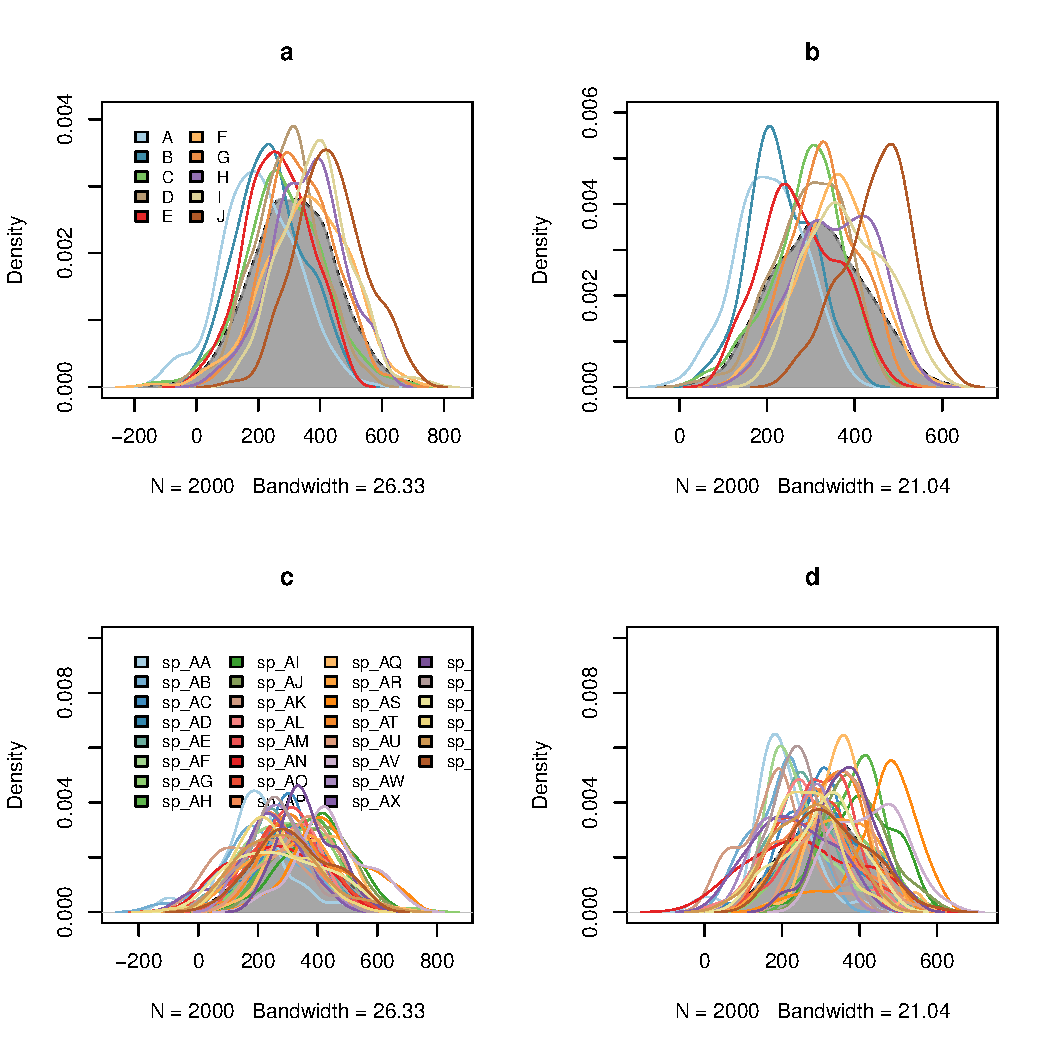
\includegraphics[width=\maxwidth]{figure/InEx_Filter_plots-1} 

}

\caption[Distribution of traits for one randomization with both internal and external filter]{Distribution of traits for one randomization with both internal and external filter: (a) Communities trait distributions for the trait a (normal distribution); (b) Communities trait distributions for the trait b (uniform distribution); (c) Species trait distributions for the trait a; (d) Species trait distributions for the trait b\label{fig:InEx_Filter_plots}}
\end{figure}


\end{knitrout}

\begin{knitrout}\small
\definecolor{shadecolor}{rgb}{0.969, 0.969, 0.969}\color{fgcolor}\begin{kframe}
\begin{alltt}
\hlkwd{par}\hlstd{(}\hlkwc{mfrow}\hlstd{=}\hlkwd{c}\hlstd{(}\hlnum{3}\hlstd{,} \hlnum{1}\hlstd{))}
\hlkwd{plot}\hlstd{(res.simu4[[}\hlnum{1}\hlstd{]],} \hlkwc{main} \hlstd{=} \hlstr{"a"}\hlstd{)}
\hlkwd{plot}\hlstd{(res.simu4[[nperm}\hlopt{/}\hlnum{2}\hlstd{]],} \hlkwc{main} \hlstd{=} \hlstr{"b"}\hlstd{)}
\hlkwd{plot}\hlstd{(res.simu4[[nperm]],} \hlkwc{main} \hlstd{=} \hlstr{"c"}\hlstd{)}
\hlkwd{par}\hlstd{(}\hlkwc{mfrow}\hlstd{=}\hlkwd{c}\hlstd{(}\hlnum{1}\hlstd{,} \hlnum{1}\hlstd{))}
\end{alltt}
\end{kframe}\begin{figure}

{\centering 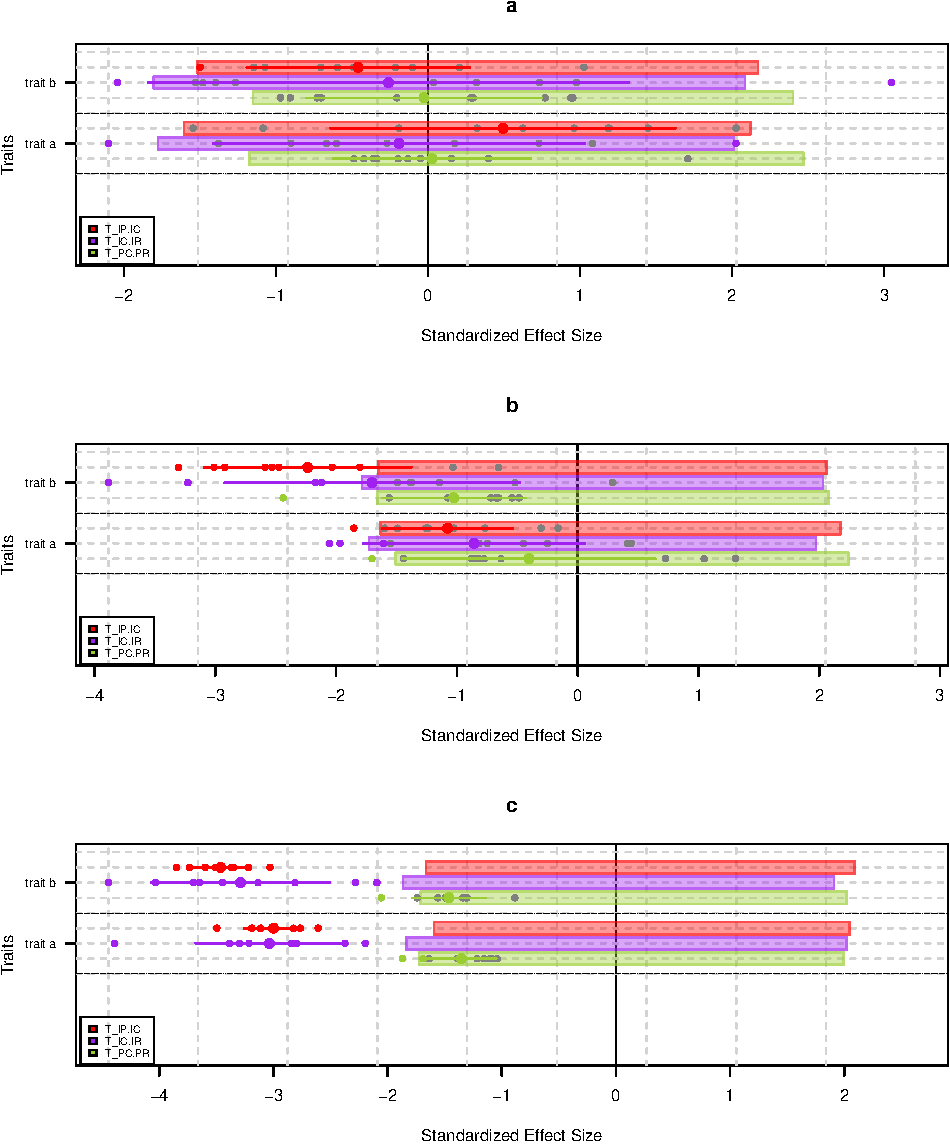
\includegraphics[width=\maxwidth]{figure/InEx_Filter_plots_Tstats-1} 

}

\caption[Results of T-statistics with both internal and external filter]{Results of T-statistics with both internal and external filter: $T_{IP/IC}$ in red, $T_{IC/IR}$ in purple and $T_{PC/PR}$ in green. (a) Lower strength of internal filtering 5 (b) higher strength of internal filtering.\label{fig:InEx_Filter_plots_Tstats}}
\end{figure}


\end{knitrout}
  

\begin{knitrout}\small
\definecolor{shadecolor}{rgb}{0.969, 0.969, 0.969}\color{fgcolor}\begin{kframe}
\begin{alltt}
\hlstd{meanSES.4loc.norm_Tipic} \hlkwb{<-} \hlkwd{unlist}\hlstd{(}\hlkwd{lapply}\hlstd{(res.simu4,} \hlkwa{function}\hlstd{(}\hlkwc{x}\hlstd{)}
             \hlkwd{ses.listofindex}\hlstd{(}\hlkwd{as.listofindex}\hlstd{(x))}
             \hlopt{$}\hlstd{index_1_1}\hlopt{$}\hlstd{ses[,} \hlnum{1}\hlstd{]))}
\hlstd{meanSES.4loc.uni_Tipic} \hlkwb{<-} \hlkwd{unlist}\hlstd{(}\hlkwd{lapply}\hlstd{(res.simu4,} \hlkwa{function}\hlstd{(}\hlkwc{x}\hlstd{)}
             \hlkwd{ses.listofindex}\hlstd{(}\hlkwd{as.listofindex}\hlstd{(x))}
             \hlopt{$}\hlstd{index_1_1}\hlopt{$}\hlstd{ses[,} \hlnum{2}\hlstd{]))}
\hlstd{SES.inf.MEAN.norm_Tipic} \hlkwb{<-} \hlkwd{unlist}\hlstd{(}\hlkwd{lapply}\hlstd{(res.simu4,} \hlkwa{function}\hlstd{(}\hlkwc{x}\hlstd{)}
             \hlkwd{ses.listofindex}\hlstd{(}\hlkwd{as.listofindex}\hlstd{(x))}
             \hlopt{$}\hlstd{index_1_1}\hlopt{$}\hlstd{ses.inf[,} \hlnum{1}\hlstd{]))}
\hlstd{SES.inf.MEAN.uni_Tipic} \hlkwb{<-} \hlkwd{unlist}\hlstd{(}\hlkwd{lapply}\hlstd{(res.simu4,} \hlkwa{function}\hlstd{(}\hlkwc{x}\hlstd{)}
             \hlkwd{ses.listofindex}\hlstd{(}\hlkwd{as.listofindex}\hlstd{(x))}
             \hlopt{$}\hlstd{index_1_1}\hlopt{$}\hlstd{ses.inf[,} \hlnum{2}\hlstd{]))}

\hlstd{meanSES.4loc.norm_Ticir} \hlkwb{<-} \hlkwd{unlist}\hlstd{(}\hlkwd{lapply}\hlstd{(res.simu4,} \hlkwa{function}\hlstd{(}\hlkwc{x}\hlstd{)}
             \hlkwd{ses.listofindex}\hlstd{(}\hlkwd{as.listofindex}\hlstd{(x))}
             \hlopt{$}\hlstd{index_1_2}\hlopt{$}\hlstd{ses[,} \hlnum{1}\hlstd{]))}
\hlstd{meanSES.4loc.uni_Ticir} \hlkwb{<-} \hlkwd{unlist}\hlstd{(}\hlkwd{lapply}\hlstd{(res.simu4,} \hlkwa{function}\hlstd{(}\hlkwc{x}\hlstd{)}
             \hlkwd{ses.listofindex}\hlstd{(}\hlkwd{as.listofindex}\hlstd{(x))}
             \hlopt{$}\hlstd{index_1_2}\hlopt{$}\hlstd{ses[,} \hlnum{2}\hlstd{]))}
\hlstd{SES.inf.MEAN.norm_Ticir} \hlkwb{<-} \hlkwd{unlist}\hlstd{(}\hlkwd{lapply}\hlstd{(res.simu4,} \hlkwa{function}\hlstd{(}\hlkwc{x}\hlstd{)}
             \hlkwd{ses.listofindex}\hlstd{(}\hlkwd{as.listofindex}\hlstd{(x))}
             \hlopt{$}\hlstd{index_1_2}\hlopt{$}\hlstd{ses.inf[,} \hlnum{1}\hlstd{]))}
\hlstd{SES.inf.MEAN.uni_Ticir} \hlkwb{<-} \hlkwd{unlist}\hlstd{(}\hlkwd{lapply}\hlstd{(res.simu4,} \hlkwa{function}\hlstd{(}\hlkwc{x}\hlstd{)}
             \hlkwd{ses.listofindex}\hlstd{(}\hlkwd{as.listofindex}\hlstd{(x))}
             \hlopt{$}\hlstd{index_1_2}\hlopt{$}\hlstd{ses.inf[,} \hlnum{2}\hlstd{]))}

\hlstd{meanSES.4loc.norm_Tpcpr} \hlkwb{<-} \hlkwd{unlist}\hlstd{(}\hlkwd{lapply}\hlstd{(res.simu4,} \hlkwa{function}\hlstd{(}\hlkwc{x}\hlstd{)}
             \hlkwd{ses.listofindex}\hlstd{(}\hlkwd{as.listofindex}\hlstd{(x))}
             \hlopt{$}\hlstd{index_1_3}\hlopt{$}\hlstd{ses[,} \hlnum{1}\hlstd{]))}
\hlstd{meanSES.4loc.uni_Tpcpr} \hlkwb{<-} \hlkwd{unlist}\hlstd{(}\hlkwd{lapply}\hlstd{(res.simu4,} \hlkwa{function}\hlstd{(}\hlkwc{x}\hlstd{)}
             \hlkwd{ses.listofindex}\hlstd{(}\hlkwd{as.listofindex}\hlstd{(x))}
             \hlopt{$}\hlstd{index_1_3}\hlopt{$}\hlstd{ses[,} \hlnum{2}\hlstd{]))}
\hlstd{SES.inf.MEAN.norm_Tpcpr} \hlkwb{<-} \hlkwd{unlist}\hlstd{(}\hlkwd{lapply}\hlstd{(res.simu4,} \hlkwa{function}\hlstd{(}\hlkwc{x}\hlstd{)}
             \hlkwd{ses.listofindex}\hlstd{(}\hlkwd{as.listofindex}\hlstd{(x))}
             \hlopt{$}\hlstd{index_1_3}\hlopt{$}\hlstd{ses.inf[,} \hlnum{1}\hlstd{]))}
\hlstd{SES.inf.MEAN.uni_Tpcpr} \hlkwb{<-} \hlkwd{unlist}\hlstd{(}\hlkwd{lapply}\hlstd{(res.simu4,} \hlkwa{function}\hlstd{(}\hlkwc{x}\hlstd{)}
             \hlkwd{ses.listofindex}\hlstd{(}\hlkwd{as.listofindex}\hlstd{(x))}
             \hlopt{$}\hlstd{index_1_3}\hlopt{$}\hlstd{ses.inf[,} \hlnum{2}\hlstd{]))}
\end{alltt}
\end{kframe}
\end{knitrout}


\begin{knitrout}\small
\definecolor{shadecolor}{rgb}{0.969, 0.969, 0.969}\color{fgcolor}\begin{kframe}
\begin{alltt}
\hlstd{meanSES.4glob.norm_Tipic} \hlkwb{<-} \hlkwd{unlist}\hlstd{(}\hlkwd{lapply}\hlstd{(res.simu4,} \hlkwa{function}\hlstd{(}\hlkwc{x}\hlstd{)}
           \hlkwd{mean}\hlstd{(}\hlkwd{ses.listofindex}\hlstd{(}\hlkwd{as.listofindex}\hlstd{(x))}
             \hlopt{$}\hlstd{index_1_1}\hlopt{$}\hlstd{ses[,}\hlnum{1}\hlstd{],} \hlkwc{na.rm} \hlstd{= T)))}
\hlstd{meanSES.4glob.uni_Tipic} \hlkwb{<-} \hlkwd{unlist}\hlstd{(}\hlkwd{lapply}\hlstd{(res.simu4,} \hlkwa{function}\hlstd{(}\hlkwc{x}\hlstd{)}
           \hlkwd{mean}\hlstd{(}\hlkwd{ses.listofindex}\hlstd{(}\hlkwd{as.listofindex}\hlstd{(x))}
             \hlopt{$}\hlstd{index_1_1}\hlopt{$}\hlstd{ses[,}\hlnum{2}\hlstd{],} \hlkwc{na.rm} \hlstd{= T)))}
\hlstd{meanSES.INF_glob.norm_Tipic} \hlkwb{<-} \hlkwd{unlist}\hlstd{(}\hlkwd{lapply}\hlstd{(res.simu4,} \hlkwa{function}\hlstd{(}\hlkwc{x}\hlstd{)}
           \hlkwd{mean}\hlstd{(}\hlkwd{ses.listofindex}\hlstd{(}\hlkwd{as.listofindex}\hlstd{(x))}
             \hlopt{$}\hlstd{index_1_1}\hlopt{$}\hlstd{ses.inf[,} \hlnum{1}\hlstd{],} \hlkwc{na.rm} \hlstd{= T)))}
\hlstd{meanSES.INF_glob.uni_Tipic} \hlkwb{<-} \hlkwd{unlist}\hlstd{(}\hlkwd{lapply}\hlstd{(res.simu4,} \hlkwa{function}\hlstd{(}\hlkwc{x}\hlstd{)}
           \hlkwd{mean}\hlstd{(}\hlkwd{ses.listofindex}\hlstd{(}\hlkwd{as.listofindex}\hlstd{(x))}
             \hlopt{$}\hlstd{index_1_1}\hlopt{$}\hlstd{ses.inf[,} \hlnum{2}\hlstd{],} \hlkwc{na.rm} \hlstd{= T)))}

\hlstd{meanSES.4glob.norm_Ticir} \hlkwb{<-} \hlkwd{unlist}\hlstd{(}\hlkwd{lapply}\hlstd{(res.simu4,} \hlkwa{function}\hlstd{(}\hlkwc{x}\hlstd{)}
           \hlkwd{mean}\hlstd{(}\hlkwd{ses.listofindex}\hlstd{(}\hlkwd{as.listofindex}\hlstd{(x))}
             \hlopt{$}\hlstd{index_1_2}\hlopt{$}\hlstd{ses[,}\hlnum{1}\hlstd{],} \hlkwc{na.rm} \hlstd{= T)))}
\hlstd{meanSES.4glob.uni_Ticir} \hlkwb{<-} \hlkwd{unlist}\hlstd{(}\hlkwd{lapply}\hlstd{(res.simu4,} \hlkwa{function}\hlstd{(}\hlkwc{x}\hlstd{)}
           \hlkwd{mean}\hlstd{(}\hlkwd{ses.listofindex}\hlstd{(}\hlkwd{as.listofindex}\hlstd{(x))}
             \hlopt{$}\hlstd{index_1_2}\hlopt{$}\hlstd{ses[,}\hlnum{2}\hlstd{],} \hlkwc{na.rm} \hlstd{= T)))}
\hlstd{meanSES.INF_glob.norm_Ticir} \hlkwb{<-} \hlkwd{unlist}\hlstd{(}\hlkwd{lapply}\hlstd{(res.simu4,} \hlkwa{function}\hlstd{(}\hlkwc{x}\hlstd{)}
           \hlkwd{mean}\hlstd{(}\hlkwd{ses.listofindex}\hlstd{(}\hlkwd{as.listofindex}\hlstd{(x))}
             \hlopt{$}\hlstd{index_1_2}\hlopt{$}\hlstd{ses.inf[,} \hlnum{1}\hlstd{],} \hlkwc{na.rm} \hlstd{= T)))}
\hlstd{meanSES.INF_glob.uni_Ticir} \hlkwb{<-} \hlkwd{unlist}\hlstd{(}\hlkwd{lapply}\hlstd{(res.simu4,} \hlkwa{function}\hlstd{(}\hlkwc{x}\hlstd{)}
           \hlkwd{mean}\hlstd{(}\hlkwd{ses.listofindex}\hlstd{(}\hlkwd{as.listofindex}\hlstd{(x))}
             \hlopt{$}\hlstd{index_1_2}\hlopt{$}\hlstd{ses.inf[,} \hlnum{2}\hlstd{],} \hlkwc{na.rm} \hlstd{= T)))}

\hlstd{meanSES.4glob.norm_Tpcpr} \hlkwb{<-} \hlkwd{unlist}\hlstd{(}\hlkwd{lapply}\hlstd{(res.simu4,} \hlkwa{function}\hlstd{(}\hlkwc{x}\hlstd{)}
           \hlkwd{mean}\hlstd{(}\hlkwd{ses.listofindex}\hlstd{(}\hlkwd{as.listofindex}\hlstd{(x))}
             \hlopt{$}\hlstd{index_1_3}\hlopt{$}\hlstd{ses[,}\hlnum{1}\hlstd{],} \hlkwc{na.rm} \hlstd{= T)))}
\hlstd{meanSES.4glob.uni_Tpcpr} \hlkwb{<-} \hlkwd{unlist}\hlstd{(}\hlkwd{lapply}\hlstd{(res.simu4,} \hlkwa{function}\hlstd{(}\hlkwc{x}\hlstd{)}
           \hlkwd{mean}\hlstd{(}\hlkwd{ses.listofindex}\hlstd{(}\hlkwd{as.listofindex}\hlstd{(x))}
             \hlopt{$}\hlstd{index_1_3}\hlopt{$}\hlstd{ses[,}\hlnum{2}\hlstd{],} \hlkwc{na.rm} \hlstd{= T)))}
\hlstd{meanSES.INF_glob.norm_Tpcpr} \hlkwb{<-} \hlkwd{unlist}\hlstd{(}\hlkwd{lapply}\hlstd{(res.simu4,} \hlkwa{function}\hlstd{(}\hlkwc{x}\hlstd{)}
           \hlkwd{mean}\hlstd{(}\hlkwd{ses.listofindex}\hlstd{(}\hlkwd{as.listofindex}\hlstd{(x))}
             \hlopt{$}\hlstd{index_1_3}\hlopt{$}\hlstd{ses.inf[,} \hlnum{1}\hlstd{],} \hlkwc{na.rm} \hlstd{= T)))}
\hlstd{meanSES.INF_glob.uni_Tpcpr} \hlkwb{<-} \hlkwd{unlist}\hlstd{(}\hlkwd{lapply}\hlstd{(res.simu4,} \hlkwa{function}\hlstd{(}\hlkwc{x}\hlstd{)}
           \hlkwd{mean}\hlstd{(}\hlkwd{ses.listofindex}\hlstd{(}\hlkwd{as.listofindex}\hlstd{(x))}
             \hlopt{$}\hlstd{index_1_3}\hlopt{$}\hlstd{ses.inf[,} \hlnum{2}\hlstd{],} \hlkwc{na.rm} \hlstd{= T)))}
\end{alltt}
\end{kframe}
\end{knitrout}



\begin{knitrout}\small
\definecolor{shadecolor}{rgb}{0.969, 0.969, 0.969}\color{fgcolor}\begin{kframe}
\begin{alltt}
\hlcom{# trait a}
\hlstd{lm_glob_norm_Tipic} \hlkwb{<-} \hlkwd{lm}\hlstd{(meanSES.4glob.norm_Tipic} \hlopt{~} \hlkwd{log}\hlstd{(init_param))}
\hlstd{lm_glob_norm_Tipic.conf} \hlkwb{<-} \hlkwd{confint}\hlstd{(lm_glob_norm_Tipic ,} \hlkwc{level} \hlstd{=} \hlnum{0.90}\hlstd{)}
\hlstd{lm_glob_norm_Ticir} \hlkwb{<-} \hlkwd{lm}\hlstd{(meanSES.4glob.norm_Ticir} \hlopt{~} \hlkwd{log}\hlstd{(init_param))}
\hlstd{lm_glob_norm_Ticir.conf} \hlkwb{<-} \hlkwd{confint}\hlstd{(lm_glob_norm_Ticir ,} \hlkwc{level} \hlstd{=} \hlnum{0.90}\hlstd{)}
\hlstd{lm_glob_norm_Tpcpr} \hlkwb{<-} \hlkwd{lm}\hlstd{(meanSES.4glob.norm_Tpcpr} \hlopt{~} \hlkwd{log}\hlstd{(init_param))}
\hlstd{lm_glob_norm_Tpcpr.conf} \hlkwb{<-} \hlkwd{confint}\hlstd{(lm_glob_norm_Tpcpr ,} \hlkwc{level} \hlstd{=} \hlnum{0.90}\hlstd{)}
\hlstd{yy.glob_norm_Tipic} \hlkwb{<-} \hlkwd{mean}\hlstd{(meanSES.INF_glob.norm_Tipic,} \hlkwc{na.rm} \hlstd{= T)}
\hlstd{yy.glob_norm_Ticir} \hlkwb{<-} \hlkwd{mean}\hlstd{(meanSES.INF_glob.norm_Ticir,} \hlkwc{na.rm} \hlstd{= T)}
\hlstd{yy.glob_norm_Tpcpr} \hlkwb{<-} \hlkwd{mean}\hlstd{(meanSES.INF_glob.norm_Tpcpr,} \hlkwc{na.rm} \hlstd{= T)}
\hlstd{param_B_glob_norm_Tipic} \hlkwb{<-} \hlkwd{exp}\hlstd{( (yy.glob_norm_Tipic} \hlopt{-} \hlstd{lm_glob_norm_Tipic.conf [}\hlnum{1}\hlstd{,} \hlnum{2}\hlstd{])} \hlopt{/}
                                  \hlstd{lm_glob_norm_Tipic.conf [}\hlnum{2}\hlstd{,} \hlnum{2}\hlstd{] )}
\hlstd{param_B_glob_norm_Ticir} \hlkwb{<-} \hlkwd{exp}\hlstd{( (yy.glob_norm_Ticir} \hlopt{-} \hlstd{lm_glob_norm_Ticir.conf [}\hlnum{1}\hlstd{,} \hlnum{2}\hlstd{])} \hlopt{/}
                                  \hlstd{lm_glob_norm_Ticir.conf [}\hlnum{2}\hlstd{,} \hlnum{2}\hlstd{] )}
\hlstd{param_B_glob_norm_Tpcpr} \hlkwb{<-} \hlkwd{exp}\hlstd{( (yy.glob_norm_Tpcpr} \hlopt{-} \hlstd{lm_glob_norm_Tpcpr.conf [}\hlnum{1}\hlstd{,} \hlnum{2}\hlstd{])} \hlopt{/}
                                  \hlstd{lm_glob_norm_Tpcpr.conf [}\hlnum{2}\hlstd{,} \hlnum{2}\hlstd{] )}

\hlstd{lm_loc_norm_Tipic} \hlkwb{<-} \hlkwd{lm}\hlstd{(meanSES.4loc.norm_Tipic} \hlopt{~} \hlkwd{log}\hlstd{(init_param.loc))}
\hlstd{lm_loc_norm_Tipic.conf} \hlkwb{<-} \hlkwd{confint}\hlstd{(lm_loc_norm_Tipic,} \hlkwc{level} \hlstd{=} \hlnum{0.90}\hlstd{)}
\hlstd{lm_loc_norm_Ticir} \hlkwb{<-} \hlkwd{lm}\hlstd{(meanSES.4loc.norm_Ticir} \hlopt{~} \hlkwd{log}\hlstd{(init_param.loc))}
\hlstd{lm_loc_norm_Ticir.conf} \hlkwb{<-} \hlkwd{confint}\hlstd{(lm_loc_norm_Ticir,} \hlkwc{level} \hlstd{=} \hlnum{0.90}\hlstd{)}
\hlstd{lm_loc_norm_Tpcpr} \hlkwb{<-} \hlkwd{lm}\hlstd{(meanSES.4loc.norm_Tpcpr} \hlopt{~} \hlkwd{log}\hlstd{(init_param.loc))}
\hlstd{lm_loc_norm_Tpcpr.conf} \hlkwb{<-} \hlkwd{confint}\hlstd{(lm_loc_norm_Tpcpr,} \hlkwc{level} \hlstd{=} \hlnum{0.90}\hlstd{)}
\hlstd{yy.loc_norm_Tipic} \hlkwb{<-} \hlkwd{mean}\hlstd{(SES.inf.MEAN.norm_Tipic,} \hlkwc{na.rm} \hlstd{= T)}
\hlstd{yy.loc_norm_Ticir} \hlkwb{<-} \hlkwd{mean}\hlstd{(SES.inf.MEAN.norm_Ticir,} \hlkwc{na.rm} \hlstd{= T)}
\hlstd{yy.loc_norm_Tpcpr} \hlkwb{<-} \hlkwd{mean}\hlstd{(SES.inf.MEAN.norm_Tpcpr,} \hlkwc{na.rm} \hlstd{= T)}
\hlstd{param_B_loc_norm_Tipic} \hlkwb{<-} \hlkwd{exp}\hlstd{( (yy.loc_norm_Tipic} \hlopt{-} \hlstd{lm_loc_norm_Tipic.conf [}\hlnum{1}\hlstd{,} \hlnum{2}\hlstd{])} \hlopt{/}
                                  \hlstd{lm_loc_norm_Tipic.conf [}\hlnum{2}\hlstd{,} \hlnum{2}\hlstd{] )}
\hlstd{param_B_loc_norm_Ticir} \hlkwb{<-} \hlkwd{exp}\hlstd{( (yy.loc_norm_Ticir} \hlopt{-} \hlstd{lm_loc_norm_Ticir.conf [}\hlnum{1}\hlstd{,} \hlnum{2}\hlstd{])} \hlopt{/}
                                  \hlstd{lm_loc_norm_Ticir.conf [}\hlnum{2}\hlstd{,} \hlnum{2}\hlstd{] )}
\hlstd{param_B_loc_norm_Tpcpr} \hlkwb{<-} \hlkwd{exp}\hlstd{( (yy.loc_norm_Tpcpr} \hlopt{-} \hlstd{lm_loc_norm_Tpcpr.conf [}\hlnum{1}\hlstd{,} \hlnum{2}\hlstd{])} \hlopt{/}
                                  \hlstd{lm_loc_norm_Tpcpr.conf [}\hlnum{2}\hlstd{,} \hlnum{2}\hlstd{] )}

\hlcom{# trait b}
\hlstd{lm_glob_uni_Tipic} \hlkwb{<-} \hlkwd{lm}\hlstd{(meanSES.4glob.uni_Tipic} \hlopt{~} \hlkwd{log}\hlstd{(init_param))}
\hlstd{lm_glob_uni_Tipic.conf} \hlkwb{<-} \hlkwd{confint}\hlstd{(lm_glob_uni_Tipic ,} \hlkwc{level} \hlstd{=} \hlnum{0.90}\hlstd{)}
\hlstd{lm_glob_uni_Ticir} \hlkwb{<-} \hlkwd{lm}\hlstd{(meanSES.4glob.uni_Ticir} \hlopt{~} \hlkwd{log}\hlstd{(init_param))}
\hlstd{lm_glob_uni_Ticir.conf} \hlkwb{<-} \hlkwd{confint}\hlstd{(lm_glob_uni_Ticir ,} \hlkwc{level} \hlstd{=} \hlnum{0.90}\hlstd{)}
\hlstd{lm_glob_uni_Tpcpr} \hlkwb{<-} \hlkwd{lm}\hlstd{(meanSES.4glob.uni_Tpcpr} \hlopt{~} \hlkwd{log}\hlstd{(init_param))}
\hlstd{lm_glob_uni_Tpcpr.conf} \hlkwb{<-} \hlkwd{confint}\hlstd{(lm_glob_uni_Tpcpr ,} \hlkwc{level} \hlstd{=} \hlnum{0.90}\hlstd{)}
\hlstd{yy.glob_uni_Tipic} \hlkwb{<-} \hlkwd{mean}\hlstd{(meanSES.INF_glob.uni_Tipic,} \hlkwc{na.rm} \hlstd{= T)}
\hlstd{yy.glob_uni_Ticir} \hlkwb{<-} \hlkwd{mean}\hlstd{(meanSES.INF_glob.uni_Ticir,} \hlkwc{na.rm} \hlstd{= T)}
\hlstd{yy.glob_uni_Tpcpr} \hlkwb{<-} \hlkwd{mean}\hlstd{(meanSES.INF_glob.uni_Tpcpr,} \hlkwc{na.rm} \hlstd{= T)}
\hlstd{param_B_glob_uni_Tipic} \hlkwb{<-} \hlkwd{exp}\hlstd{( (yy.glob_uni_Tipic} \hlopt{-} \hlstd{lm_glob_uni_Tipic.conf [}\hlnum{1}\hlstd{,} \hlnum{2}\hlstd{])} \hlopt{/}
                                  \hlstd{lm_glob_uni_Tipic.conf [}\hlnum{2}\hlstd{,} \hlnum{2}\hlstd{] )}
\hlstd{param_B_glob_uni_Ticir} \hlkwb{<-} \hlkwd{exp}\hlstd{( (yy.glob_uni_Ticir} \hlopt{-} \hlstd{lm_glob_uni_Ticir.conf [}\hlnum{1}\hlstd{,} \hlnum{2}\hlstd{])} \hlopt{/}
                                  \hlstd{lm_glob_uni_Ticir.conf [}\hlnum{2}\hlstd{,} \hlnum{2}\hlstd{] )}
\hlstd{param_B_glob_uni_Tpcpr} \hlkwb{<-} \hlkwd{exp}\hlstd{( (yy.glob_uni_Tpcpr} \hlopt{-} \hlstd{lm_glob_uni_Tpcpr.conf [}\hlnum{1}\hlstd{,} \hlnum{2}\hlstd{])} \hlopt{/}
                                  \hlstd{lm_glob_uni_Tpcpr.conf [}\hlnum{2}\hlstd{,} \hlnum{2}\hlstd{] )}

\hlstd{lm_loc_uni_Tipic} \hlkwb{<-} \hlkwd{lm}\hlstd{(meanSES.4loc.uni_Tipic} \hlopt{~} \hlkwd{log}\hlstd{(init_param.loc))}
\hlstd{lm_loc_uni_Tipic.conf} \hlkwb{<-} \hlkwd{confint}\hlstd{(lm_loc_uni_Tipic,} \hlkwc{level} \hlstd{=} \hlnum{0.90}\hlstd{)}
\hlstd{lm_loc_uni_Ticir} \hlkwb{<-} \hlkwd{lm}\hlstd{(meanSES.4loc.uni_Ticir} \hlopt{~} \hlkwd{log}\hlstd{(init_param.loc))}
\hlstd{lm_loc_uni_Ticir.conf} \hlkwb{<-} \hlkwd{confint}\hlstd{(lm_loc_uni_Ticir,} \hlkwc{level} \hlstd{=} \hlnum{0.90}\hlstd{)}
\hlstd{lm_loc_uni_Tpcpr} \hlkwb{<-} \hlkwd{lm}\hlstd{(meanSES.4loc.uni_Tpcpr} \hlopt{~} \hlkwd{log}\hlstd{(init_param.loc))}
\hlstd{lm_loc_uni_Tpcpr.conf} \hlkwb{<-} \hlkwd{confint}\hlstd{(lm_loc_uni_Tpcpr,} \hlkwc{level} \hlstd{=} \hlnum{0.90}\hlstd{)}
\hlstd{yy.loc_uni_Tipic} \hlkwb{<-} \hlkwd{mean}\hlstd{(SES.inf.MEAN.uni_Tipic,} \hlkwc{na.rm} \hlstd{= T)}
\hlstd{yy.loc_uni_Ticir} \hlkwb{<-} \hlkwd{mean}\hlstd{(SES.inf.MEAN.uni_Ticir,} \hlkwc{na.rm} \hlstd{= T)}
\hlstd{yy.loc_uni_Tpcpr} \hlkwb{<-} \hlkwd{mean}\hlstd{(SES.inf.MEAN.uni_Tpcpr,} \hlkwc{na.rm} \hlstd{= T)}
\hlstd{param_B_loc_uni_Tipic} \hlkwb{<-} \hlkwd{exp}\hlstd{( (yy.loc_uni_Tipic} \hlopt{-} \hlstd{lm_loc_uni_Tipic.conf [}\hlnum{1}\hlstd{,} \hlnum{2}\hlstd{])} \hlopt{/}
                                  \hlstd{lm_loc_uni_Tipic.conf [}\hlnum{2}\hlstd{,} \hlnum{2}\hlstd{] )}
\hlstd{param_B_loc_uni_Ticir} \hlkwb{<-} \hlkwd{exp}\hlstd{( (yy.loc_uni_Ticir} \hlopt{-} \hlstd{lm_loc_uni_Ticir.conf [}\hlnum{1}\hlstd{,} \hlnum{2}\hlstd{])} \hlopt{/}
                                  \hlstd{lm_loc_uni_Ticir.conf [}\hlnum{2}\hlstd{,} \hlnum{2}\hlstd{] )}
\hlstd{param_B_loc_uni_Tpcpr} \hlkwb{<-} \hlkwd{exp}\hlstd{( (yy.loc_uni_Tpcpr} \hlopt{-} \hlstd{lm_loc_uni_Tpcpr.conf [}\hlnum{1}\hlstd{,} \hlnum{2}\hlstd{])} \hlopt{/}
                                  \hlstd{lm_loc_uni_Tpcpr.conf [}\hlnum{2}\hlstd{,} \hlnum{2}\hlstd{] )}
\end{alltt}
\end{kframe}
\end{knitrout}

For the analysis with both internal and external filter we only present the type II error using the initial parameter ratio allowing a beta-error $<0.05$.  

\begin{table}[h!]
\begin{center}
\caption{Initial parameter ratio allowing beta-error $<0.05$ for T-statistics under both external and internal filtering}
\begin{tabular}{|c|c|c|c|m{6cm}|}
\hline
Traits & Indices & Average between communities? & Initial parameter ratio$ \tabularnewline
\hline \hline \hline
\multirow{6}{*}{Trait a (normal)} & \multirow{2}{*}{$T_{IP.IC}$} & no (local) & 1.515 \tabularnewline
\cline{3-4} 
 & & yes (global) & 1.541 \tabularnewline
\cline{2-4} 
 & \multirow{2}{*}{$T_{IC.IR}$} & no (local) & 5.224 \tabularnewline
\cline{3-4} 
 & & yes (global) & 5.492 \tabularnewline
\cline{2-4} 
 & \multirow{2}{*}{$T_{PC.PR}$} & no (local) & 133.91 \tabularnewline
\cline{3-4}
 & & yes (global)& 150.875 \tabularnewline

\hline \hline \hline

\multirow{6}{*}{Trait b (uniform)} & \multirow{2}{*}{$T_{IP.IC}$} & no (local) & 0.413 \tabularnewline
\cline{3-4}
 & & yes (global) &  0.398 \tabularnewline
\cline{2-4} 
 & \multirow{2}{*}{$T_{IC.IR}$} & no (local) & 1.01 \tabularnewline
\cline{3-4} 
 & & yes (global) &  1.023 \tabularnewline
\cline{2-4} 
 & \multirow{2}{*}{$T_{PC.PR}$} & no (local) & 44.917 \tabularnewline
\cline{3-4} 
 & & yes (global)&  52.127 \tabularnewline
\hline 
\end{tabular}
\end{center}
\end{table}























\cleardoublepage

\section{Test of variance decomposition functions}
 
In addition to the \texttt{cati} vignette that test this function on the Darwin finch data, we test the behavior of the function \texttt{partvar} and \texttt{decompCTRE} by building two toy models associated to each functions.
 
 \subsection{Behavior of the function \texttt{partvar}}

First to test the behavior of the \texttt{partvar} function we assemble the same data as in the test of the T-statistics. 
1000 individuals belonging to 20 species occuring in 10 communities. But here we define the trait value for one individual as the addition of three values, each one draw in a normal distribution of mean 0 and standard error 1: (i) a value depending of the species the individual belong to, (ii) a value depending of the community the individual belong to and (iii) a independent value measuring the individual variance.

\begin{knitrout}\small
\definecolor{shadecolor}{rgb}{0.969, 0.969, 0.969}\color{fgcolor}\begin{kframe}
\begin{alltt}
\hlstd{nperm} \hlkwb{<-} \hlstd{npermut}

\hlstd{sdlog} \hlkwb{=} \hlnum{1.5}
\hlcom{#Ten communities named A, B, C ... J}
\hlstd{com} \hlkwb{<-} \hlkwd{c}\hlstd{(}\hlstr{"A"}\hlstd{,} \hlstr{"B"}\hlstd{,} \hlstr{"C"}\hlstd{,} \hlstr{"D"}\hlstd{,} \hlstr{"E"}\hlstd{,} \hlstr{"F"}\hlstd{,} \hlstr{"G"}\hlstd{,} \hlstr{"H"}\hlstd{,} \hlstr{"I"}\hlstd{,} \hlstr{"J"}\hlstd{)}
\hlcom{#Twenty species sp1, sp2, sp3, ... sp20}
\hlstd{sp} \hlkwb{<-} \hlkwd{paste}\hlstd{(}\hlstr{"sp"}\hlstd{,} \hlkwd{seq}\hlstd{(}\hlnum{1}\hlopt{:}\hlnum{20}\hlstd{),} \hlkwc{sep} \hlstd{=} \hlstr{""}\hlstd{)}

\hlstd{res.partvar_toymodel} \hlkwb{<-} \hlkwd{list}\hlstd{()}
\hlkwa{for}\hlstd{(n} \hlkwa{in} \hlnum{1}\hlopt{:}\hlstd{nperm)\{}\hlcom{#for each permutation}

 \hlcom{# Draw communities using lognormal distribution of abondances }
 \hlcom{# 100 individuals by populations}
 \hlstd{ex.sp5} \hlkwb{<-} \hlkwd{c}\hlstd{()}
 \hlstd{ex.com5} \hlkwb{<-} \hlkwd{matrix}\hlstd{(}\hlnum{0}\hlstd{,} \hlkwc{nrow} \hlstd{=} \hlnum{10}\hlstd{,} \hlkwc{ncol} \hlstd{=} \hlnum{20}\hlstd{)}
 \hlkwa{for}\hlstd{(i} \hlkwa{in} \hlnum{1}\hlopt{:} \hlnum{10}\hlstd{)\{}
 \hlstd{ex.com.interm} \hlkwb{<-} \hlkwd{table}\hlstd{(}\hlkwd{sample}\hlstd{(sp,} \hlkwc{size} \hlstd{=} \hlnum{100}\hlstd{,} \hlkwc{prob} \hlstd{=} \hlkwd{rlnorm}\hlstd{(}\hlnum{20}\hlstd{,} \hlnum{0}\hlstd{, sdlog),} \hlkwc{replace} \hlstd{= T))}
 \hlstd{ex.com5[i, sp}\hlopt \hlkwd{names}\hlstd{(ex.com.interm)]} \hlkwb{<-} \hlstd{ex.com.interm}
 \hlstd{ex.sp5} \hlkwb{<-} \hlkwd{c}\hlstd{(ex.sp5,} \hlkwd{rep}\hlstd{(sp,} \hlkwc{times} \hlstd{= ex.com5[i,]))}
 \hlstd{\}}


 \hlstd{x1} \hlkwb{<-} \hlkwd{c}\hlstd{()}
 \hlstd{ex.sp5} \hlkwb{<-} \hlkwd{as.factor}\hlstd{(ex.sp5)}
 \hlkwa{for}\hlstd{(s} \hlkwa{in} \hlnum{1}\hlopt{:}\hlnum{20}\hlstd{)\{}
 \hlstd{x1[ex.sp5} \hlopt{==} \hlkwd{levels}\hlstd{(ex.sp5)[s]]} \hlkwb{<-} \hlkwd{rnorm}\hlstd{(}\hlnum{1}\hlstd{)}
 \hlstd{\}}

 \hlstd{ex.indplot5} \hlkwb{<-} \hlkwd{as.factor}\hlstd{(}\hlkwd{rep}\hlstd{(com,} \hlnum{100}\hlstd{))}
 \hlstd{x2} \hlkwb{<-} \hlkwd{c}\hlstd{()}
 \hlstd{x3} \hlkwb{<-} \hlkwd{c}\hlstd{()}
 \hlstd{ex.indplot5} \hlkwb{<-} \hlkwd{as.factor}\hlstd{(ex.indplot5 )}
 \hlkwa{for}\hlstd{(c} \hlkwa{in} \hlnum{1}\hlopt{:}\hlnum{10}\hlstd{)\{}
 \hlstd{x2[ex.indplot5} \hlopt{==} \hlkwd{levels}\hlstd{(ex.indplot5 )[c]]} \hlkwb{<-} \hlkwd{rnorm}\hlstd{(}\hlnum{1}\hlstd{)}
 \hlstd{\}}
 \hlstd{X} \hlkwb{<-} \hlkwd{rnorm}\hlstd{(}\hlnum{1000}\hlstd{)} \hlopt{+} \hlstd{x1} \hlopt{+} \hlstd{x2}

 \hlstd{res.partvar_toymodel[[n]]} \hlkwb{<-} \hlkwd{partvar}\hlstd{(X,} \hlkwc{factors} \hlstd{=} \hlkwd{cbind}\hlstd{(}\hlkwc{sites} \hlstd{= ex.indplot5,}
               \hlkwc{species} \hlstd{= ex.sp5))}
\hlstd{\}}
\end{alltt}
\end{kframe}
\end{knitrout}

Now we can plot the result as the density of the three component of variation in individual traits distributions. 
We are waiting for a mean of approximately 0.33 for each component in view of our model.

\begin{knitrout}\small
\definecolor{shadecolor}{rgb}{0.969, 0.969, 0.969}\color{fgcolor}\begin{kframe}
\begin{alltt}
\hlstd{res.simu.partvar_toymodel} \hlkwb{<-} \hlkwd{lapply}\hlstd{(res.partvar_toymodel,} \hlkwa{function} \hlstd{(}\hlkwc{x}\hlstd{) x[,} \hlnum{1}\hlstd{])}
\hlstd{res.simu.partvar_toymodel} \hlkwb{<-} \hlkwd{t}\hlstd{(}\hlkwd{matrix}\hlstd{(}\hlkwd{unlist}\hlstd{(res.simu.partvar_toymodel),} \hlkwc{nrow} \hlstd{=} \hlnum{3}\hlstd{))}
\hlkwd{colnames}\hlstd{(res.simu.partvar_toymodel)} \hlkwb{<-} \hlkwd{c}\hlstd{(}\hlstr{"sites"}\hlstd{,} \hlstr{"species"}\hlstd{,} \hlstr{"within"}\hlstd{)}
\hlstd{col.funk} \hlkwb{<-} \hlkwd{funky.col}\hlstd{(}\hlnum{3}\hlstd{)}

\hlkwd{plot}\hlstd{(}\hlkwd{density}\hlstd{(res.simu.partvar_toymodel[,} \hlnum{3}\hlstd{]),} \hlkwc{col} \hlstd{= col.funk[}\hlnum{3}\hlstd{],}
  \hlkwc{pch} \hlstd{=} \hlnum{16}\hlstd{,} \hlkwc{xlim} \hlstd{=} \hlkwd{c}\hlstd{(}\hlnum{0}\hlstd{,} \hlnum{0.9}\hlstd{),} \hlkwc{lwd} \hlstd{=} \hlnum{2}\hlstd{)}
\hlkwd{lines}\hlstd{(}\hlkwd{density}\hlstd{(res.simu.partvar_toymodel[,} \hlnum{1}\hlstd{]),} \hlkwc{col} \hlstd{= col.funk[}\hlnum{1}\hlstd{],} \hlkwc{lwd} \hlstd{=} \hlnum{2}\hlstd{)}
\hlkwd{lines}\hlstd{(}\hlkwd{density}\hlstd{(res.simu.partvar_toymodel[,} \hlnum{2}\hlstd{]),} \hlkwc{col} \hlstd{= col.funk[}\hlnum{2}\hlstd{],} \hlkwc{lwd} \hlstd{=} \hlnum{2}\hlstd{)}
\hlkwd{abline}\hlstd{(}\hlkwc{v} \hlstd{=} \hlnum{0.33}\hlstd{)}
\hlkwd{points}\hlstd{(}\hlkwd{apply}\hlstd{(res.simu.partvar_toymodel,} \hlnum{2}\hlstd{, mean),}
   \hlkwd{c}\hlstd{(}\hlkwd{max}\hlstd{(}\hlkwd{density}\hlstd{(res.simu.partvar_toymodel[,} \hlnum{1}\hlstd{])}\hlopt{$}\hlstd{y)}\hlopt{/}\hlnum{2}\hlstd{,}
   \hlkwd{max}\hlstd{(}\hlkwd{density}\hlstd{(res.simu.partvar_toymodel[,} \hlnum{2}\hlstd{])}\hlopt{$}\hlstd{y)}\hlopt{/}\hlnum{2}\hlstd{,}
   \hlkwd{max}\hlstd{(}\hlkwd{density}\hlstd{(res.simu.partvar_toymodel[,} \hlnum{3}\hlstd{])}\hlopt{$}\hlstd{y)}\hlopt{/}\hlnum{2}\hlstd{),}
   \hlkwc{col} \hlstd{= col.funk)}
\hlkwd{segments}\hlstd{(}\hlkwd{apply}\hlstd{(res.simu.partvar_toymodel,} \hlnum{2}\hlstd{, mean)} \hlopt{-} \hlkwd{apply}\hlstd{(res.simu.partvar_toymodel,} \hlnum{2}\hlstd{, sd),}
   \hlkwd{c}\hlstd{(}\hlkwd{max}\hlstd{(}\hlkwd{density}\hlstd{(res.simu.partvar_toymodel[,} \hlnum{1}\hlstd{])}\hlopt{$}\hlstd{y)}\hlopt{/}\hlnum{2}\hlstd{,}
   \hlkwd{max}\hlstd{(}\hlkwd{density}\hlstd{(res.simu.partvar_toymodel[,} \hlnum{2}\hlstd{])}\hlopt{$}\hlstd{y)}\hlopt{/}\hlnum{2}\hlstd{,}
   \hlkwd{max}\hlstd{(}\hlkwd{density}\hlstd{(res.simu.partvar_toymodel[,} \hlnum{3}\hlstd{])}\hlopt{$}\hlstd{y)}\hlopt{/}\hlnum{2}\hlstd{),}
   \hlkwd{apply}\hlstd{(res.simu.partvar_toymodel,} \hlnum{2}\hlstd{, mean)} \hlopt{+} \hlkwd{apply}\hlstd{(res.simu.partvar_toymodel,} \hlnum{2}\hlstd{, sd),}
   \hlkwd{c}\hlstd{(}\hlkwd{max}\hlstd{(}\hlkwd{density}\hlstd{(res.simu.partvar_toymodel[,} \hlnum{1}\hlstd{])}\hlopt{$}\hlstd{y)}\hlopt{/}\hlnum{2}\hlstd{,}
   \hlkwd{max}\hlstd{(}\hlkwd{density}\hlstd{(res.simu.partvar_toymodel[,} \hlnum{2}\hlstd{])}\hlopt{$}\hlstd{y)}\hlopt{/}\hlnum{2}\hlstd{,}
   \hlkwd{max}\hlstd{(}\hlkwd{density}\hlstd{(res.simu.partvar_toymodel[,} \hlnum{3}\hlstd{])}\hlopt{$}\hlstd{y)}\hlopt{/}\hlnum{2}\hlstd{),}
   \hlkwc{col} \hlstd{= col.funk)}
\hlkwd{legend}\hlstd{(}\hlnum{0.6}\hlstd{,} \hlnum{4}\hlstd{,} \hlkwc{legend} \hlstd{=} \hlkwd{c}\hlstd{(}\hlstr{"sites"}\hlstd{,} \hlstr{"species"}\hlstd{,} \hlstr{"within"}\hlstd{),} \hlkwc{fill} \hlstd{= col.funk)}
\hlkwd{text}\hlstd{(}\hlnum{0.33}\hlstd{,} \hlnum{0.5}\hlstd{,} \hlkwc{pos} \hlstd{=} \hlnum{4}\hlstd{,} \hlstr{"0.33"}\hlstd{)}
\end{alltt}
\end{kframe}\begin{figure}

{\centering 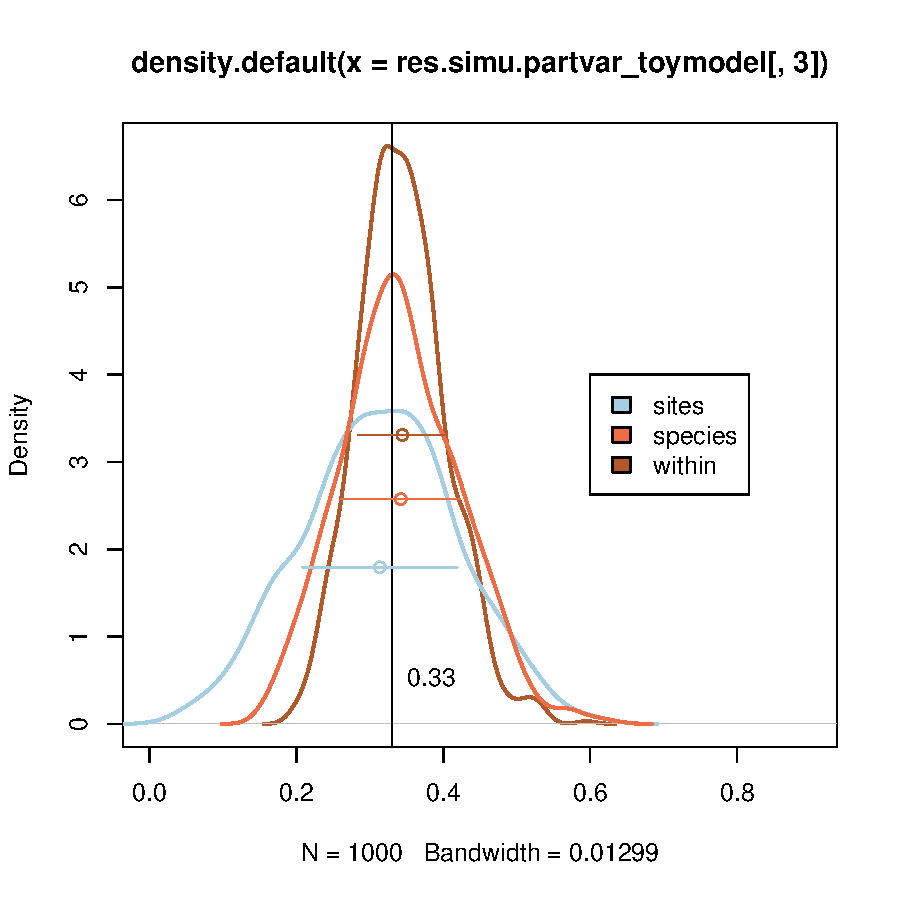
\includegraphics[width=\maxwidth]{figure/Partvar_plot-1} 

}

\caption[Variance partitioning accross nested scales]{Variance partitioning accross nested scales: each colored lines represent the density of permutations results (sites in blue, species in orange and the remaining variance in brown). Points represent the mean and segments the standard deviation. Vertical line figure the value of 0.33.\label{fig:Partvar_plot}}
\end{figure}


\end{knitrout}

The mean contribution of each component is near 0.33. Consequently the function \texttt{partvar} don't show apparent dysfunction.

\subsection{Behavior of the function \texttt{decompCTRE}}

To test the function \texttt{decompCTRE}, we adopt the same model but we add a new step to control the strength of the turnover in defining the community weighted mean.
We define several value of turnover strength by deleting individuals from the data set if there their species-components trait and their community-component trait are to different. To be more precise, when \texttt{turnover\_strength} = 1, we delete all individual whose the square of the species value minus the community value is superior o one. 

\begin{knitrout}\small
\definecolor{shadecolor}{rgb}{0.969, 0.969, 0.969}\color{fgcolor}\begin{kframe}
\begin{alltt}
\hlstd{sdlog} \hlkwb{=} \hlnum{1.5}
\hlstd{turnover_strength} \hlkwb{<-} \hlkwd{rep}\hlstd{(}\hlkwd{c}\hlstd{(}\hlnum{0.01}\hlstd{,} \hlnum{0.1}\hlstd{,} \hlnum{0.2}\hlstd{,} \hlnum{0.5}\hlstd{,} \hlnum{1}\hlstd{,} \hlnum{2}\hlstd{,} \hlnum{3.5}\hlstd{,} \hlnum{5}\hlstd{,} \hlnum{7.5}\hlstd{,} \hlnum{10}\hlstd{,} \hlnum{12.5}\hlstd{,} \hlnum{15}\hlstd{),}
                         \hlstd{N_repet_Param)}
\hlstd{nperm} \hlkwb{<-} \hlkwd{length}\hlstd{(turnover_strength)}
\hlstd{res.decompCTRE_toymodel} \hlkwb{<-} \hlkwd{list}\hlstd{()}
\hlkwa{for}\hlstd{(n} \hlkwa{in} \hlnum{1}\hlopt{:}\hlstd{nperm)\{}\hlcom{#for each permutation}

 \hlcom{# Draw communities using lognormal distribution of abondances }
 \hlcom{# 100 individuals by populations}
 \hlstd{ex.sp5} \hlkwb{<-} \hlkwd{c}\hlstd{()}
 \hlstd{ex.com5} \hlkwb{<-} \hlkwd{matrix}\hlstd{(}\hlnum{0}\hlstd{,} \hlkwc{nrow} \hlstd{=} \hlnum{10}\hlstd{,} \hlkwc{ncol} \hlstd{=} \hlnum{20}\hlstd{)}
 \hlkwa{for}\hlstd{(i} \hlkwa{in} \hlnum{1}\hlopt{:} \hlnum{10}\hlstd{)\{}
 \hlstd{ex.com.interm} \hlkwb{<-} \hlkwd{table}\hlstd{(}\hlkwd{sample}\hlstd{(sp,} \hlkwc{size} \hlstd{=} \hlnum{100}\hlstd{,} \hlkwc{prob} \hlstd{=} \hlkwd{rlnorm}\hlstd{(}\hlnum{20}\hlstd{,} \hlnum{0}\hlstd{, sdlog),} \hlkwc{replace} \hlstd{= T))}
 \hlstd{ex.com5[i, sp}\hlopt \hlkwd{names}\hlstd{(ex.com.interm)]} \hlkwb{<-} \hlstd{ex.com.interm}
 \hlstd{ex.sp5} \hlkwb{<-} \hlkwd{c}\hlstd{(ex.sp5,} \hlkwd{rep}\hlstd{(sp,} \hlkwc{times} \hlstd{= ex.com5[i,]))}
 \hlstd{\}}


 \hlstd{x1} \hlkwb{<-} \hlkwd{c}\hlstd{()}
 \hlstd{ex.sp5} \hlkwb{<-} \hlkwd{as.factor}\hlstd{(ex.sp5)}
 \hlkwa{for}\hlstd{(s} \hlkwa{in} \hlnum{1}\hlopt{:}\hlnum{20}\hlstd{)\{}
 \hlstd{x1[ex.sp5} \hlopt{==} \hlkwd{levels}\hlstd{(ex.sp5)[s]]} \hlkwb{<-} \hlkwd{rnorm}\hlstd{(}\hlnum{1}\hlstd{)}
 \hlstd{\}}

 \hlstd{ex.indplot5} \hlkwb{<-} \hlkwd{as.factor}\hlstd{(}\hlkwd{rep}\hlstd{(com,} \hlnum{100}\hlstd{))}
 \hlstd{x2} \hlkwb{<-} \hlkwd{c}\hlstd{()}
 \hlstd{ex.indplot5} \hlkwb{<-} \hlkwd{as.factor}\hlstd{(ex.indplot5)}
 \hlkwa{for}\hlstd{(c} \hlkwa{in} \hlnum{1}\hlopt{:}\hlnum{10}\hlstd{)\{}
 \hlstd{x2[ex.indplot5} \hlopt{==} \hlkwd{levels}\hlstd{(ex.indplot5)[c]]} \hlkwb{<-} \hlkwd{rnorm}\hlstd{(}\hlnum{1}\hlstd{)}
 \hlstd{\}}

 \hlstd{X} \hlkwb{<-} \hlkwd{rnorm}\hlstd{(}\hlnum{1000}\hlstd{)} \hlopt{+} \hlstd{x1} \hlopt{+} \hlstd{x2}

 \hlcom{#We delete the individual whose species values and communities values are to different}
 \hlcom{#For this we use the argument turnover_strength}
 \hlstd{X2} \hlkwb{<-} \hlstd{X[(x1}\hlopt{-}\hlstd{x2)}\hlopt{^}\hlnum{2} \hlopt{<} \hlstd{turnover_strength[n]]}
 \hlstd{ex.sp5.bis} \hlkwb{<-} \hlstd{ex.sp5[(x1}\hlopt{-}\hlstd{x2)}\hlopt{^}\hlnum{2} \hlopt{<} \hlstd{turnover_strength[n]]}
 \hlstd{ex.indplot5.bis} \hlkwb{<-} \hlstd{ex.indplot5[(x1}\hlopt{-}\hlstd{x2)}\hlopt{^}\hlnum{2} \hlopt{<} \hlstd{turnover_strength[n]]}

 \hlstd{res.decompCTRE_toymodel[[n]]} \hlkwb{<-} \hlkwd{decompCTRE}\hlstd{(}\hlkwc{traits} \hlstd{=} \hlkwd{cbind}\hlstd{(X2, X2),} \hlkwc{sp} \hlstd{= ex.sp5.bis,}
            \hlkwc{ind.plot} \hlstd{= ex.indplot5.bis)}
\hlstd{\}}\hlcom{#End of simulation}
\end{alltt}
\end{kframe}
\end{knitrout}
Now we can plot the relation between the modeled strength of the turnover and the resulting contribution of turnover from the function \texttt{decompCTRE} (Fig. \ref{fig:decompCTRE_plot1}).

\begin{knitrout}\small
\definecolor{shadecolor}{rgb}{0.969, 0.969, 0.969}\color{fgcolor}\begin{kframe}
\begin{alltt}
\hlkwd{par}\hlstd{(}\hlkwc{mfrow}\hlstd{=}\hlkwd{c}\hlstd{(}\hlnum{1}\hlstd{,} \hlnum{2}\hlstd{))}
\hlkwd{plot}\hlstd{(res.decompCTRE_toymodel[[}\hlnum{1}\hlstd{]]}\hlopt{$}\hlstd{X2)}
\hlkwd{plot}\hlstd{(res.decompCTRE_toymodel[[n]]}\hlopt{$}\hlstd{X2)}
\hlkwd{par}\hlstd{(}\hlkwc{mfrow}\hlstd{=}\hlkwd{c}\hlstd{(}\hlnum{1}\hlstd{,} \hlnum{1}\hlstd{))}
\end{alltt}
\end{kframe}\begin{figure}

{\centering 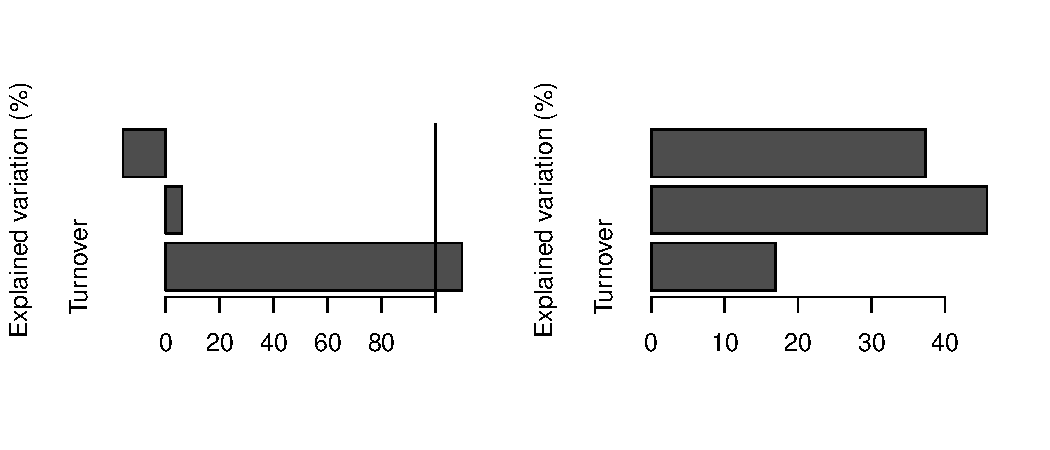
\includegraphics[width=\maxwidth]{figure/decompCTRE_plot1-1} 

}

\caption[Decomposition of the variation in community trait composition for two contrasted cases]{Decomposition of the variation in community trait composition for two contrasted cases: on the left almost all the variation is due to turnover wheras on the rigth case intraspecific variation explain most of the variation.\label{fig:decompCTRE_plot1}}
\end{figure}


\end{knitrout}

\begin{knitrout}\small
\definecolor{shadecolor}{rgb}{0.969, 0.969, 0.969}\color{fgcolor}\begin{kframe}
\begin{alltt}
\hlstd{res.simu.decompCTRE_toymodel} \hlkwb{<-} \hlkwd{unlist}\hlstd{(}\hlkwd{lapply}\hlstd{(res.decompCTRE_toymodel,} \hlkwa{function}\hlstd{(}\hlkwc{x}\hlstd{)}
                                              \hlstd{x}\hlopt{$}\hlstd{X2}\hlopt{$}\hlstd{RelSumSq[}\hlnum{1}\hlstd{]))}
\hlkwd{plot}\hlstd{(res.simu.decompCTRE_toymodel,} \hlopt{-}\hlstd{turnover_strength,} \hlkwc{pch} \hlstd{=} \hlnum{16}\hlstd{,} \hlkwc{col} \hlstd{=} \hlkwd{rgb}\hlstd{(}\hlnum{0}\hlstd{,} \hlnum{0}\hlstd{,} \hlnum{0}\hlstd{,} \hlnum{0.5}\hlstd{),}
     \hlkwc{ylab} \hlstd{=} \hlstr{"Strength of the turnover (maximum strength = 0)"}\hlstd{,}
     \hlkwc{xlab} \hlstd{=} \hlstr{"Turnover relative contribution to community mean traits"}\hlstd{)}
\end{alltt}
\end{kframe}\begin{figure}

{\centering 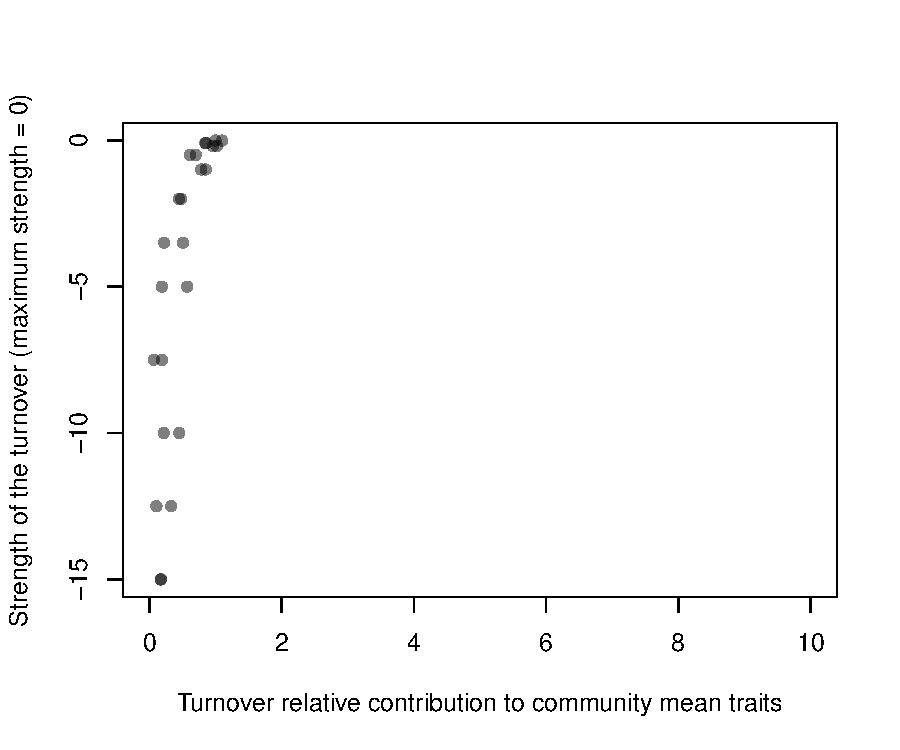
\includegraphics[width=\maxwidth]{figure/decompCTRE_plot2-1} 

}

\caption[Modeled against obtained turnover contribution in community trait variance]{Modeled against obtained turnover contribution in community trait variance\label{fig:decompCTRE_plot2}}
\end{figure}


\end{knitrout}

The correlation between the modeled strength of the turnover and the turnover relative contribution result is very high. Consequently the function \texttt{decompCTRE} don't show apparent dysfunction (Fig. \ref{fig:decompCTRE_plot2}).

\cleardoublepage


\section{Summary}
\label{sect:summary}

\subsection{Type I error}

Table \ref{tab:Alpha-errors_for_T-stats} summarize the alpha error for T-statistics. The three global \footnote{one indice for all the dataset} T-statistics are very robust 
regardless of the distribution of the trait (alpha error ranging from 0.001 to 0.001). Local \footnote{one indice for each community of the dataset} T-statistics present lower but nevertheless satifactory alpha-error with a maximum of 0.04035 for $T_{PC/PR}$ on a trait normally distributed. We therefore recommand to use $T_{IC/IR}$ to detect external filtering and more generally to prefer global T-statistics which are more robust and more powerfull (see the next section).


\subsection{Type II error}


\begin{table}[h!]
\begin{center}
\caption{Summary of initial parameter ratio allowing beta-error $<0.05$ for global T-statistics}
\begin{tabular}{|c|c|>{\centering}m{3cm}|>{\centering}m{3cm}|>{\centering}m{3cm}|}
\hline
Traits & Indices & Initial parameter ratio with internal filtering & Initial parameter ratio with external filtering & Initial parameter ratio with internal and external filtering \tabularnewline
\hline \hline \hline

\multirow{3}{*}{Trait a (normal)} & $T_{IP.IC}$ & 1.05 & \cellcolor{ligthgray}  & 1.54\tabularnewline
\cline{2-5} 
 & $T_{IC.IR}$ & \cellcolor{ligthgray} & 1.07 &  5.49 \tabularnewline
\cline{2-5}
 & $T_{PC.PR}$ & \cellcolor{ligthgray} & 1.62 &  150.88 \tabularnewline

\hline \hline \hline


Traits & Indices & Initial parameter ratio with internal filtering & Initial parameter ratio with external filtering & Initial parameter ratio with internal and external filtering \tabularnewline
\hline \hline \hline

\multirow{3}{*}{Trait b (uniform)} & $T_{IP.IC}$ & 0.51 & \cellcolor{ligthgray} & 0.4\tabularnewline
\cline{2-5} 
 & $T_{IC.IR}$ & \cellcolor{ligthgray} & 0.51 &  1.02 \tabularnewline
\cline{2-5}
 & $T_{PC.PR}$ & \cellcolor{ligthgray} & 0.78 &  52.13 \tabularnewline


\hline 
\end{tabular}
\end{center}
\end{table}








\section*{Conclusion}
\addcontentsline{toc}{subsection}{Conclusion}

\section*{References}
\addcontentsline{toc}{subsection}{References}
May RM, Mac Arthur RH (1972) Niche overlap as a function of environmental variability. Proceedings of the National Academy of Sciences 69: 1109-1113.
\\

Violle C, Enquist BJ, McGill BJ, Jiang L, Albert CH, et al. (2012) The return of the variance: intraspecific variability in community ecology. Trends in Ecology & Evolution 27: 244-252.


\listoffigures % table des figures
\listoftables % table des tableaux


\end{document}



%%%%%%%%%%%%%%%%%%%%%%%%%%%%%%%%%%%%%%%%%%%%%%%%%%
%%%%%%%%%%%%%%%%%%%%%%%%%%%%%%%%%%%%%%%%%%%%%%%%%%
%%%%%%%%%%%%%%%%%%%%%%%%%%%%%%%%%%%%%%%%%%%%%%%%%%

